\section*{Introduction}\index{Hymenoptera}
This unit focuses on \textbf{Hymenoptera}, a lineage of almost indescribable diversity (155,000 known species and probably at least a million that need names). Is this the largest order? Possibly \citep{forbes2018quantifying}. These species, commonly known as sawflies, wasps, bees, and ants, exhibit a broad array of morphologies and life histories. Their ecological and economic importance, as predators (\textit{e.g.}, ants), pollinators (bees), pests (\textit{e.g.}, some herbivorous sawflies), and bio-control agents (numerous parasitic wasps) is enormous. Members of this order can be readily separated from other insects based on the following characteristics:

\begin{itemize}
\item haplodiploidy (males are haploid)
\item smaller hind wings connected to larger fore wings by hook-like spurs (\latinword{hamuli})
\item transverse and longitudinal veins cannot be differentiated (compare with Odonata and Plecoptera, \textit{e.g.}, where transverse veins are usually less sclerotized and more flexible than longitudinal veins)
\item protibial apical spur and the first basitarsus is modified into an antenna cleaning device
\item abdominal tergite I at least partly fused with metanotum
\end{itemize}

\section{Hymenoptera}
\subsection{Non-apocritan Hymenoptera (``Symphyta'')}\index{Symphyta}
\noindent{}\textit{Diagnostic characters:} Body in dorsal view with very little or no constriction near its middle between abdominal segments 1 and 2 (\textit{i.e}., ``wasp waist'' absent; figure \ref{fig:symphyt1}); cenchrus usually present (arrows in figure \ref{fig:symphyt1}); fore tibia with two apical spurs; never less than 3 mm in length; first abdominal tergite usually divided medially.\vspace{3mm}

\noindent{}\textit{Natural history:} Non-apocritans, known commonly as ``sawflies'', are generally phyto-phagous as larvae. One important exception is the family Orussidae (figure \ref{fig:orussid1}; not covered in lab), which are parasitoids. Orussidae is understood to be sister to the megadiverse lineage called Apocrita.

\begin{figure}[ht!]
    \centering
    \begin{subfigure}[ht!]{0.47\textwidth}
        \reflectbox{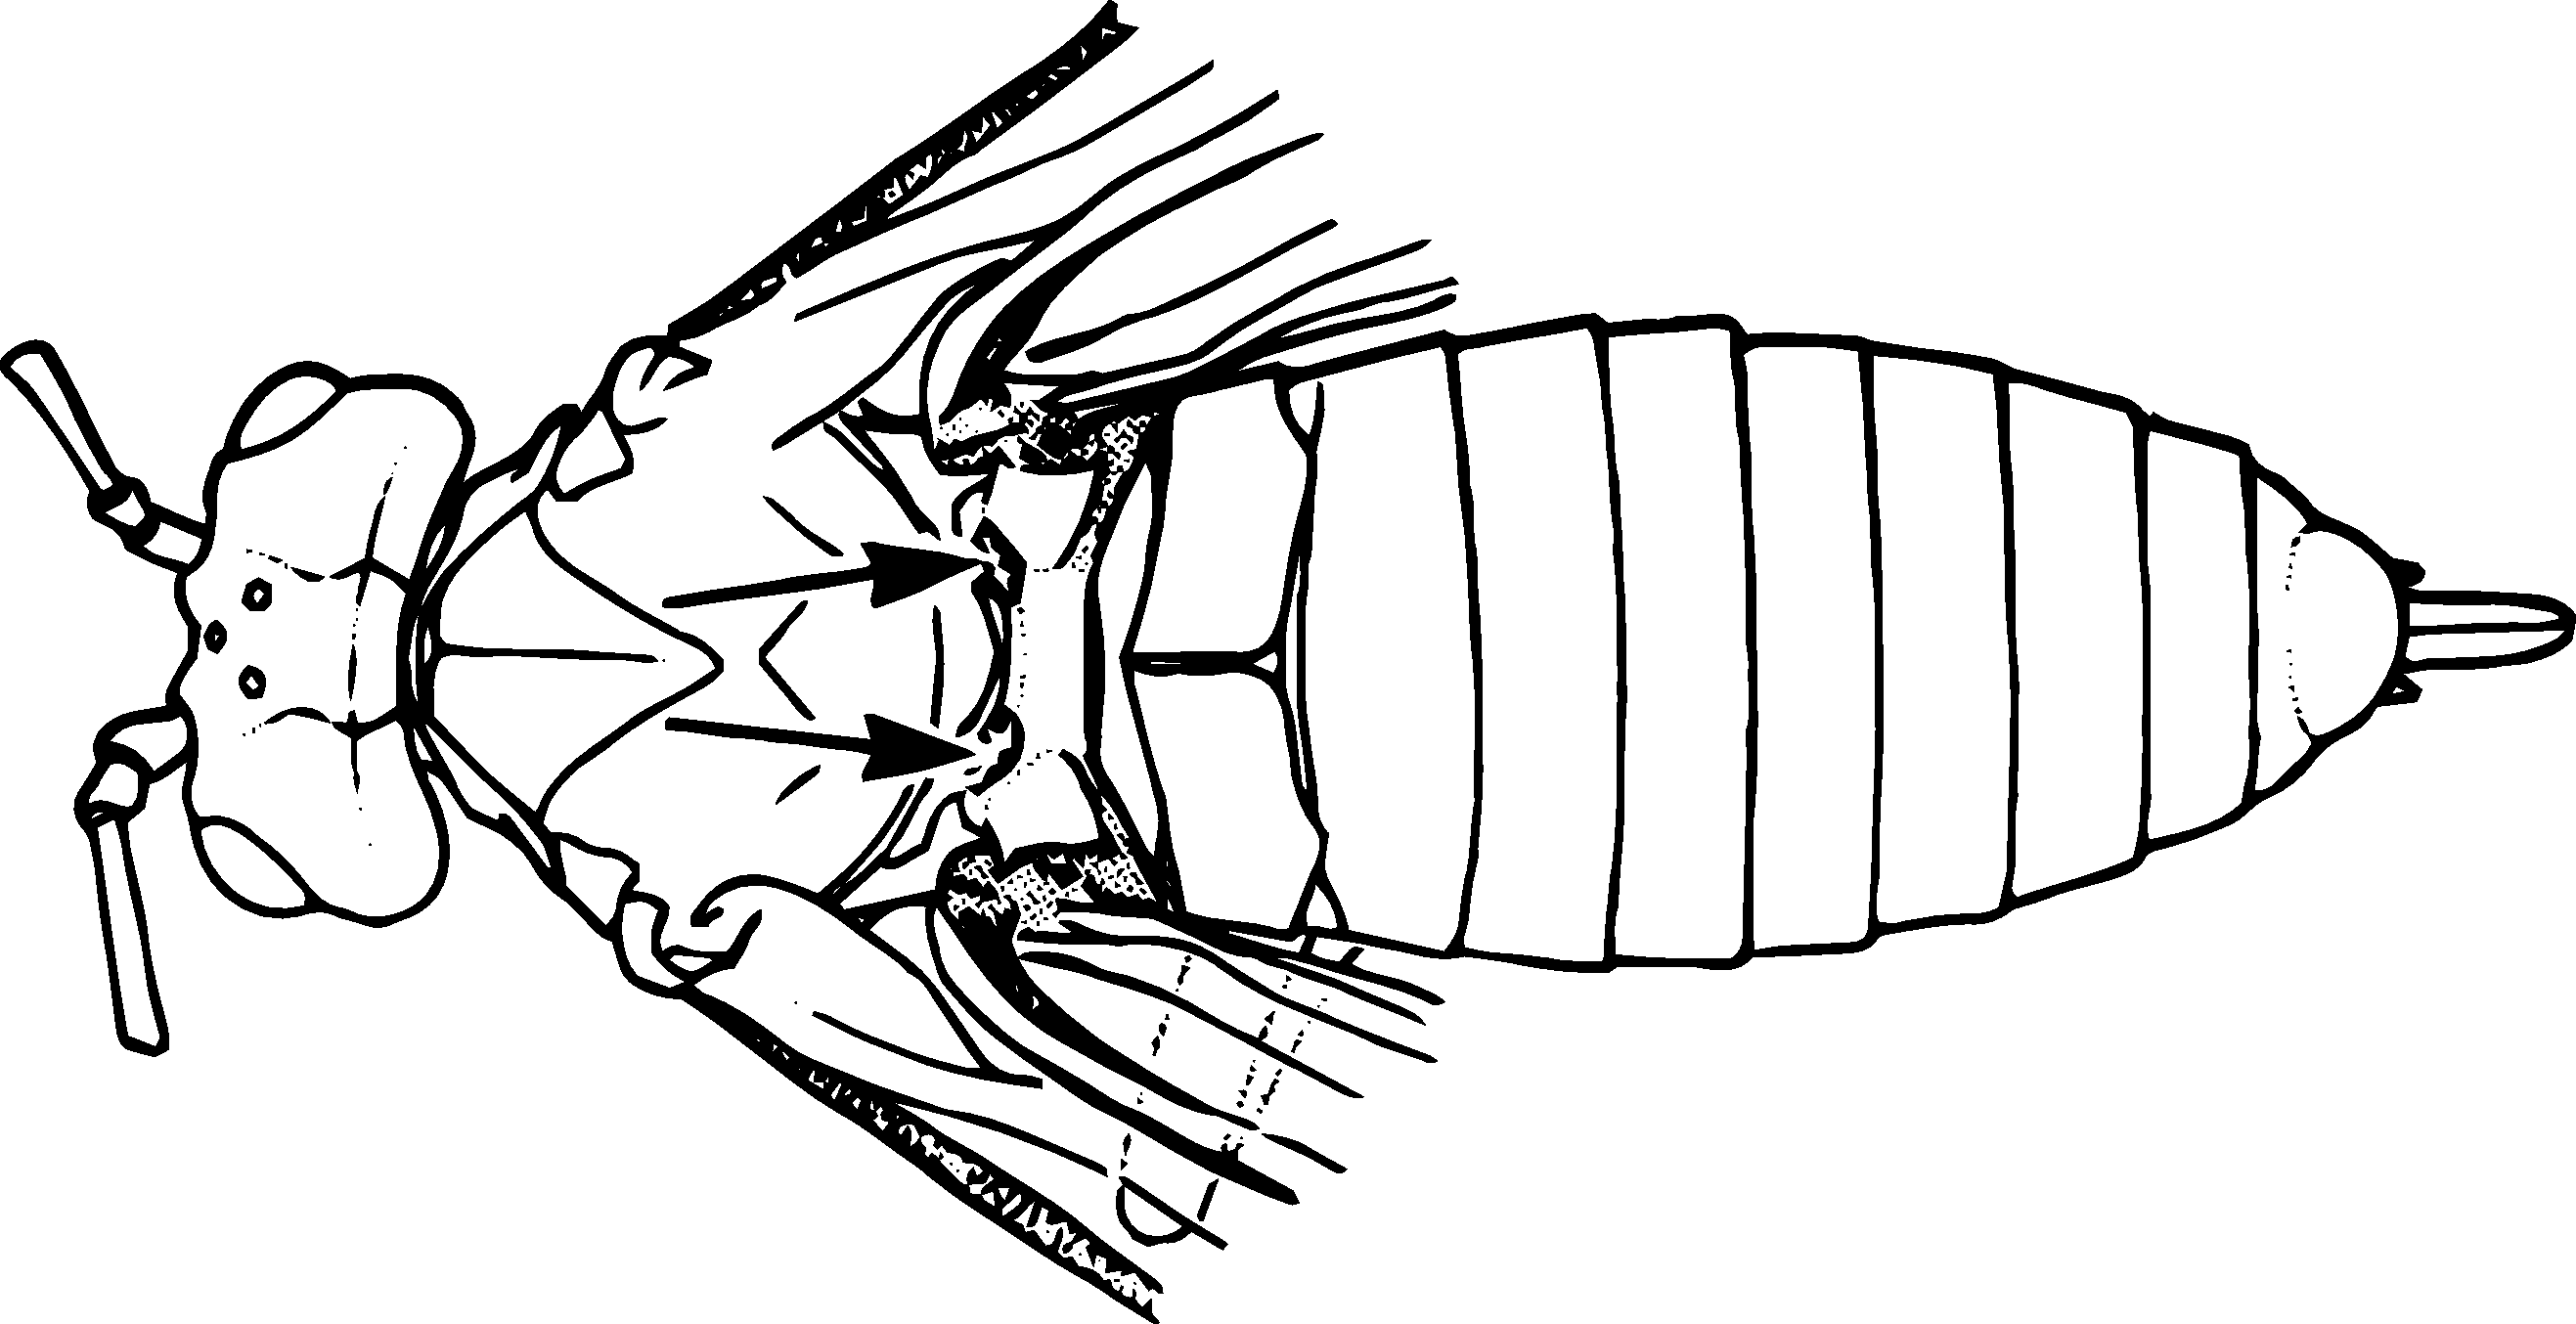
\includegraphics[width=\textwidth]{hymenoptera/SymphytaHabitus}}
        \caption{Symphytan dorsal habitus}
        \label{fig:symphyt1}
    \end{subfigure}
    \hfill 
    \begin{subfigure}[ht!]{0.45\textwidth}
        \reflectbox{\includegraphics[width=\textwidth]{hymenoptera/OrussidHabitus}}
        \caption{Orussidae habitus}
        \label{fig:orussid1}
    \end{subfigure}
    \caption{\citep[][Pg. 42, Fig. 24]{goulet1993hymenoptera}; }\label{fig:symphytans}
\end{figure}

\subsubsection{Xyelidae}\index{Xyelidae}
\noindent{}\textit{Diagnostic characters:} Antennae with less than 10 flagellomeres; proximal-most flagellomere much longer than following flagellomeres; maxillary palp leg-like (figure \ref{fig:xyelids}).\vspace{3mm}

\noindent{}\textit{Natural history:} Larvae develop inside pollen-producing cones of pine trees (\textit{Pinus} spp.), while adults can be found very early in the spring, feeding on pine and other tree pollen. The oldest hymenopteran fossils (Triassic) look almost like extant xyelids. There are approximately 50 spp.

\begin{figure}[ht!]
    \centering
    \begin{subfigure}[ht!]{0.4\textwidth}
        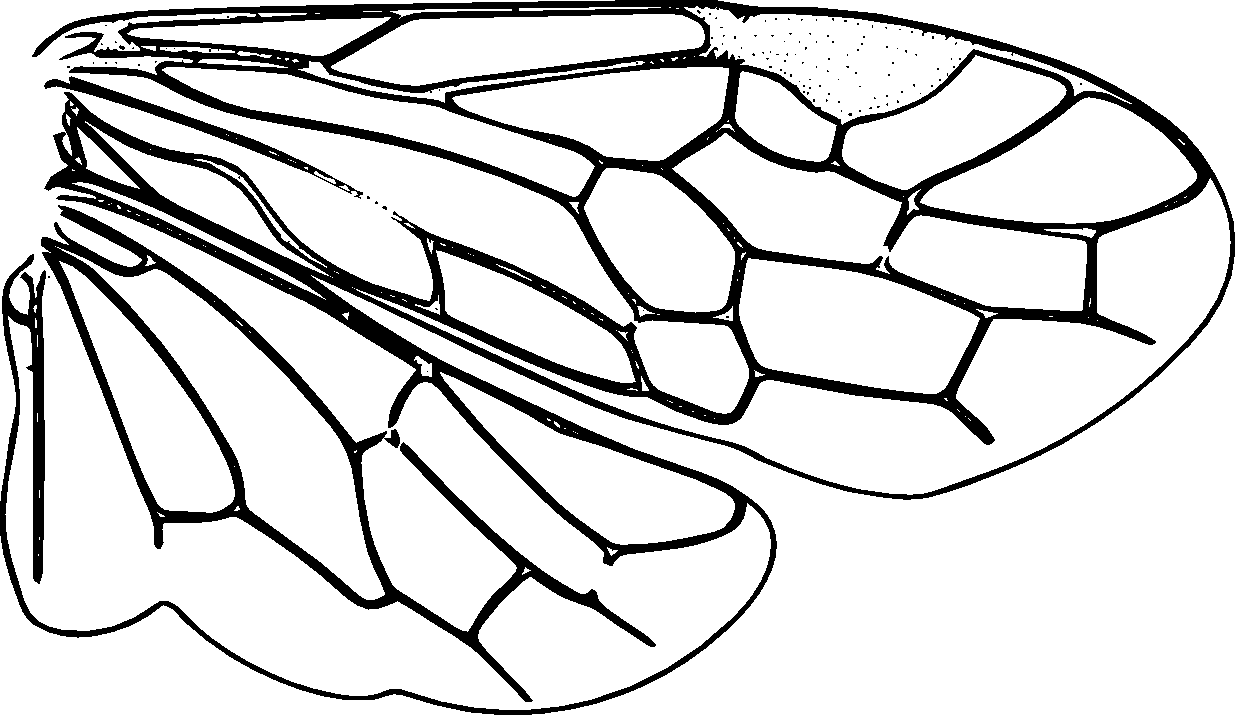
\includegraphics[width=\textwidth]{hymenoptera/XyelidWings}
        \caption{}
        \label{fig:xyelidwings}
    \end{subfigure}
    \hfill 
    \begin{subfigure}[ht!]{0.42\textwidth}
        \reflectbox{\includegraphics[width=\textwidth]{hymenoptera/XyelidHabitus}}
        \caption{}
        \label{fig:xyelidhead}
    \end{subfigure}
    \caption{Xyelidae. \textbf{(a)} Wings \citep[][modified from Fig. 32]{goulet1993hymenoptera}; \textbf{(b)} habitus \citep[][Fig. 32]{goulet1993hymenoptera}}\label{fig:xyelids}
\end{figure}

\subsubsection{Diprionidae (conifer sawflies)}\index{Diprionidae}
\noindent{}\textit{Diagnostic characters:} Antenna with $\sim$20 flagellomeres, comb-like in males and saw-like in females; fore wing with less than 2 marginal cells; abdominal tergum 1 separated from metapleuron in both sexes.\vspace{3mm}

\noindent{}\textit{Natural history:} Larvae develop as folivores on pines. Some species are considered pests. Larvae often feed gregariously, regurgitating pine resin when disturbed. Almost 100 species have been described.

\begin{figure}[ht!]
    \centering
    \begin{subfigure}[ht!]{0.14\textwidth}
        \includegraphics[width=\textwidth]{hymenoptera/DiprionidAntenna}
        \caption{}
        \label{fig:diprionid1}
    \end{subfigure}
    \qquad
    \begin{subfigure}[ht!]{0.42\textwidth}
        \reflectbox{\includegraphics[width=\textwidth]{hymenoptera/DiprionidHabitus}}
        \caption{}
        \label{fig:diprionid2}
    \end{subfigure}
    \caption{Diprionidae. \textbf{(a)} Male antenna \citep[][pg. 108]{goulet1993hymenoptera}; \textbf{(b)} habitus \citep[][Fig. 29]{goulet1993hymenoptera}}\label{fig:diprion}
\end{figure}

\subsubsection{Tenthredinidae (common sawflies)}\index{Tenthredinidae}
\noindent{}\textit{Diagnostic characters:} Antenna with 3--7 flagellomeres (figure \ref{fig:tenthred1}); abdominal tergum 1 clearly separated from metapleuron.\vspace{3mm}

\noindent{}\textit{Natural history:} Larvae are diversely phytophagous, developing as folivores, borers, gallers, and even leaf miners. There are more than 7,000 described spp.

\begin{figure}[ht!]
  \centering
    \reflectbox{\includegraphics[width=0.4\textwidth]{hymenoptera/TenthredinidHabitus}}
  \caption{Tenthredinidae, lateral habitus \citep[][Fig. 31]{goulet1993hymenoptera}}
  \label{fig:tenthred1}
\end{figure}

\noindent{}The next family represents a transition in life history, from larvae feeding mostly on leaves to larvae feeding inside wood.\vspace{3mm}

\begin{theo}
{}Can you see evidence of this transition in the external morphology of these hymenopterans? Compare Siricidae to Tenthredinidae, for example, and describe or illustrate a few differences. %What is the function of the transcutal articulation?
\end{theo}

\subsubsection{Siricidae (horntails)}\index{Siricidae}
\noindent{}\textit{Diagnostic characters:} Antenna with \textgreater{}20 flagellomeres; pronotum with a large dorsal (horizontal) surface (figure \ref{fig:siricid1}); fore tibia with one apical spur; posterior-most tergum in females and sternum in males with apical projection (figure \ref{fig:siricid2})\vspace{3mm}

\noindent{}\textit{Natural history:} There are $\sim$150 described species. Female siricids have pockets (\latinword{mycangia}; we'll see this word again when we cover Coleoptera) at the base of their ovipositors that contain fungi.

\begin{theo}
{}What do you think is the role of the symbiotic fungi found in siricids?
\end{theo}

\begin{figure}[ht!]
    \centering
    \begin{subfigure}[ht!]{0.36\textwidth}
        \reflectbox{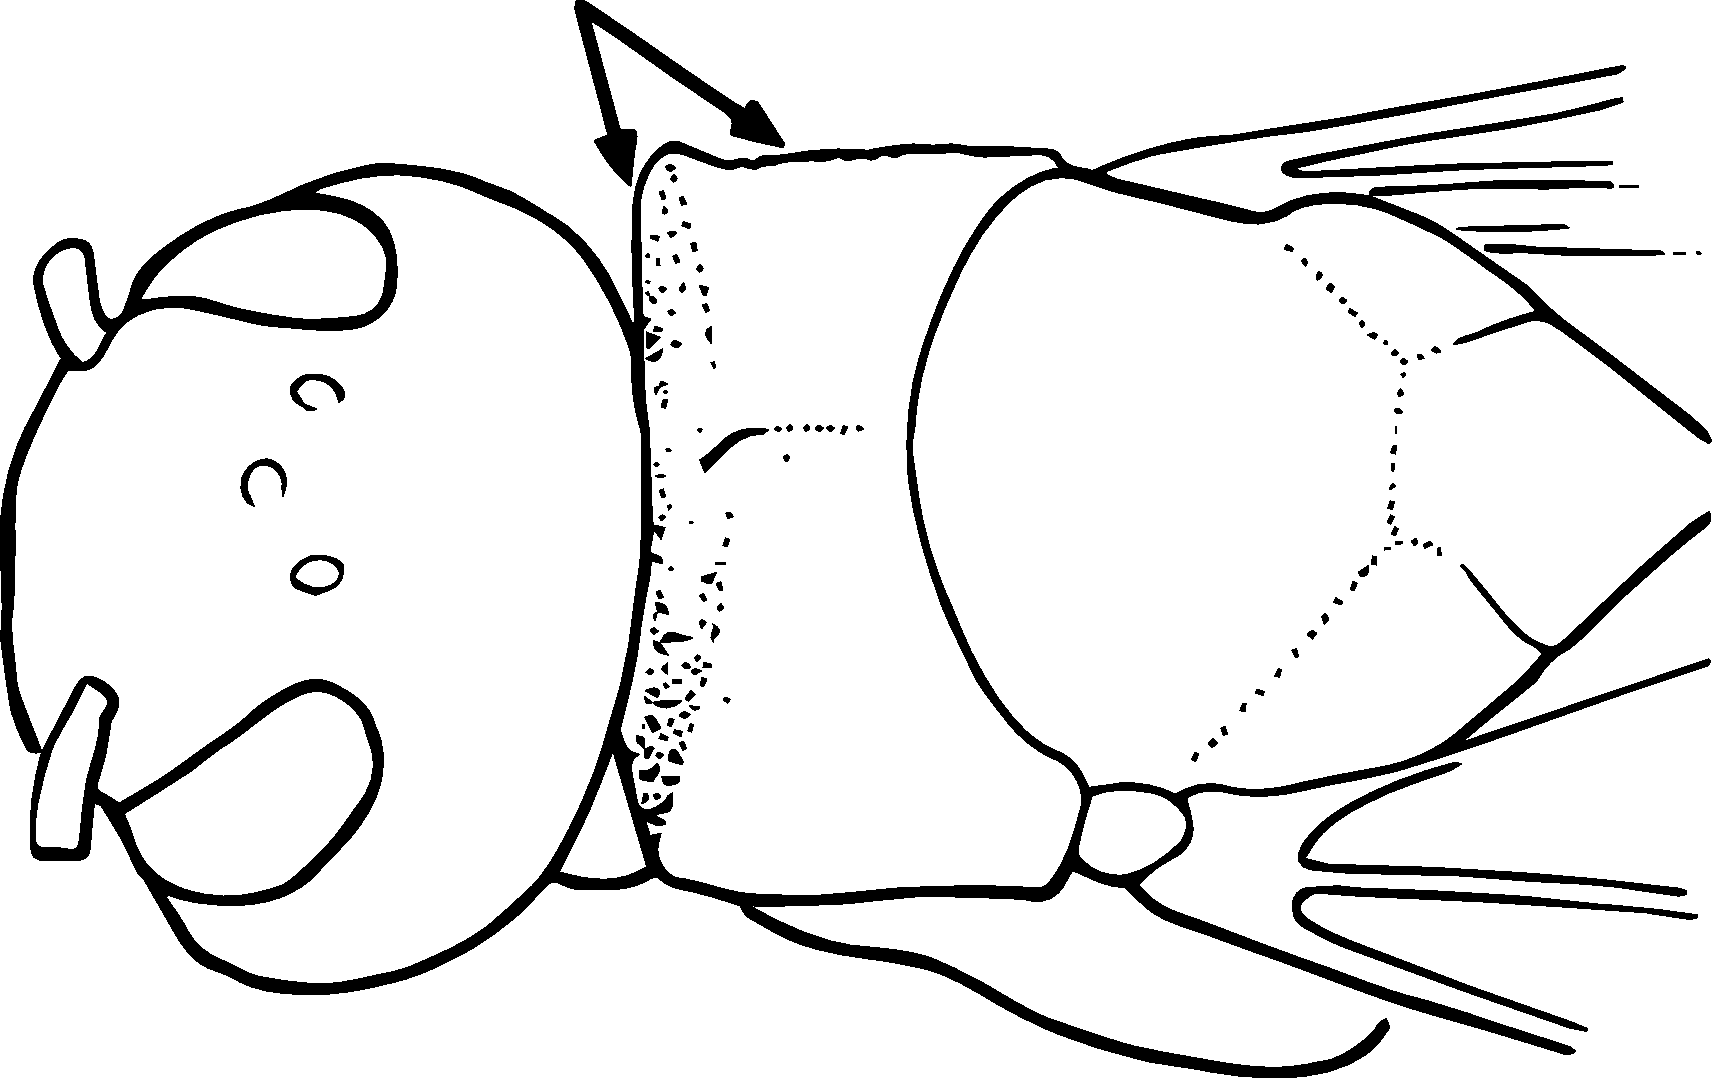
\includegraphics[width=\textwidth]{hymenoptera/SiricidPronotum}}
        \caption{}
        \label{fig:siricid1}
    \end{subfigure}
    \hfill
    \begin{subfigure}[ht!]{0.42\textwidth}
        \reflectbox{\includegraphics[width=\textwidth]{hymenoptera/SiricidHabitus}}
        \caption{}
        \label{fig:siricid2}
    \end{subfigure}
    \caption{Siricidae. \textbf{(a)} Dorsal head and thorax \citep[][pg. 70]{goulet1993hymenoptera}; \textbf{(b)} habitus \citep[][Fig. 25]{goulet1993hymenoptera}}\label{fig:siricids}
\end{figure}

\subsection{Apocrita}\index{Apocrita}
The remaining hymenopterans comprise the megadiverse Apocrita, a lineage characterized in part, at least ancestrally, by developing as parasitoids of other insects. In dorsal view, the body has a distinct constriction near its middle (\textit{i.e.}, ``wasp waist'' present); note that the middle tagma is referred to as the \latinword{mesosoma} and the posteriormost tagma is the \latinword{metasoma}.

\subsubsection{Evaniidae (ensign or hatchet wasps)}\index{Evaniidae}
\noindent{}\textit{Diagnostic characters:} Antenna with 13 antennomeres (one neotropical genus has 10); pterostigma relatively small; mesosoma relatively stout; hind wing with jugal lobe; metasoma arising dorsally on mesosoma, distance between propodeal foramen and metacoxal cavity much larger than width of either opening; metasoma hatchet-shaped; petiole tubular.\vspace{3mm}

\noindent{}\textit{Natural history:} These wasps develop as solitary predators of cockroach eggs, inside the ootheca. Approximately 550 species have been described, but only a handful occur in North America.

\begin{figure}[ht!]
  \centering
\begin{subfigure}[ht!]{0.4\textwidth}
    \reflectbox{\includegraphics[width=\textwidth]{hymenoptera/EvaniidHabitus}}
  \caption{}
  \label{fig:evaniid1}
\end{subfigure}
    \hfill
\begin{subfigure}[ht!]{0.45\textwidth}
    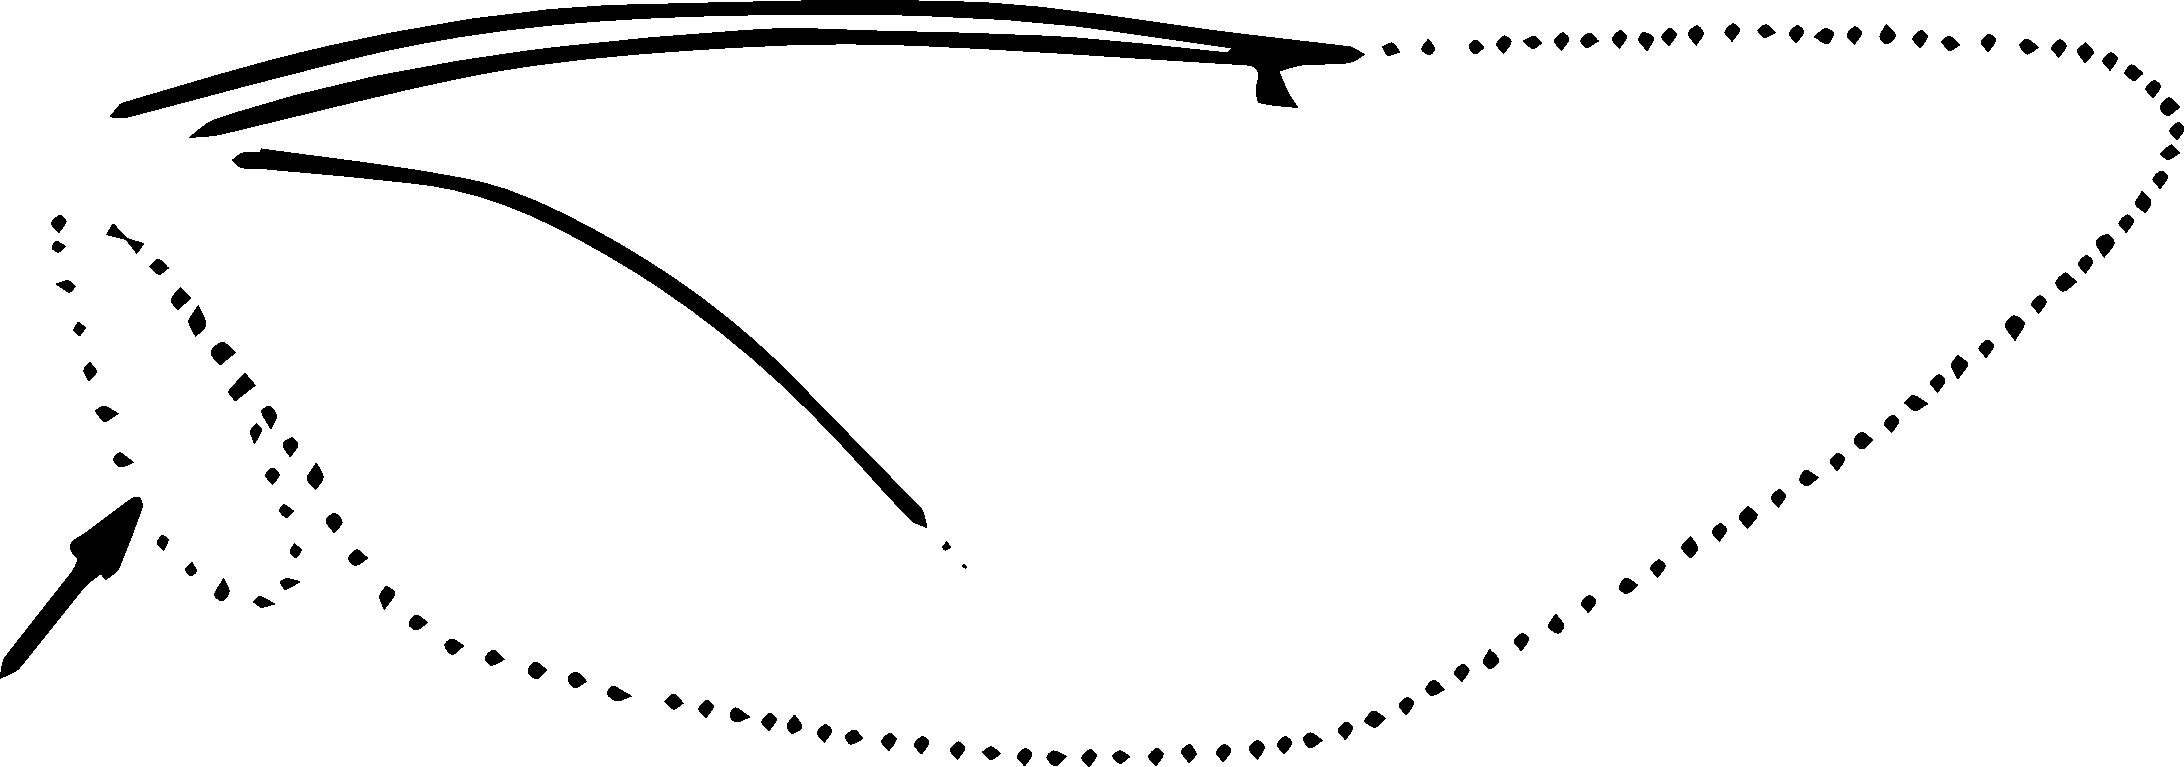
\includegraphics[width=\textwidth]{hymenoptera/EvaniidWing}
  \caption{}
  \label{fig:evaniid2}
\end{subfigure}
    \caption{Evaniidae. \textbf{(a)} Lateral habitus (illustration by A. R. Deans); \textbf{(b)} hind wing \citep[][pg. 510]{goulet1993hymenoptera}}
    \label{fig:evaniid}
\end{figure}

\subsubsection{Megaspilidae}\index{Megaspilidae}
\noindent{}\textit{Diagnostic characters:} Antenna with 12 antennomeres (figure \ref{fig:megaspilid2}); fore wing with no cells enclosed by tubular veins (figure \ref{fig:megaspilid1})and only 1 proximal tubular vein on anterior margin; pterostigma distinct; protibia with two apical spurs; pronotum adjacent to tegula in lateral view (compare to Chalcidoidea).\vspace{3mm}

\noindent{}\textit{Natural history:} Parasitoids of many kinds of insects, including other parasitoid Hymenoptera (\textit{i.e.}, some megaspilids are hyperparasitoids). These wasps are relatively easy to collect, and there are just over 300 species known worldwide.

\begin{figure}[ht!]
  \centering
\begin{subfigure}[ht!]{0.45\textwidth}
    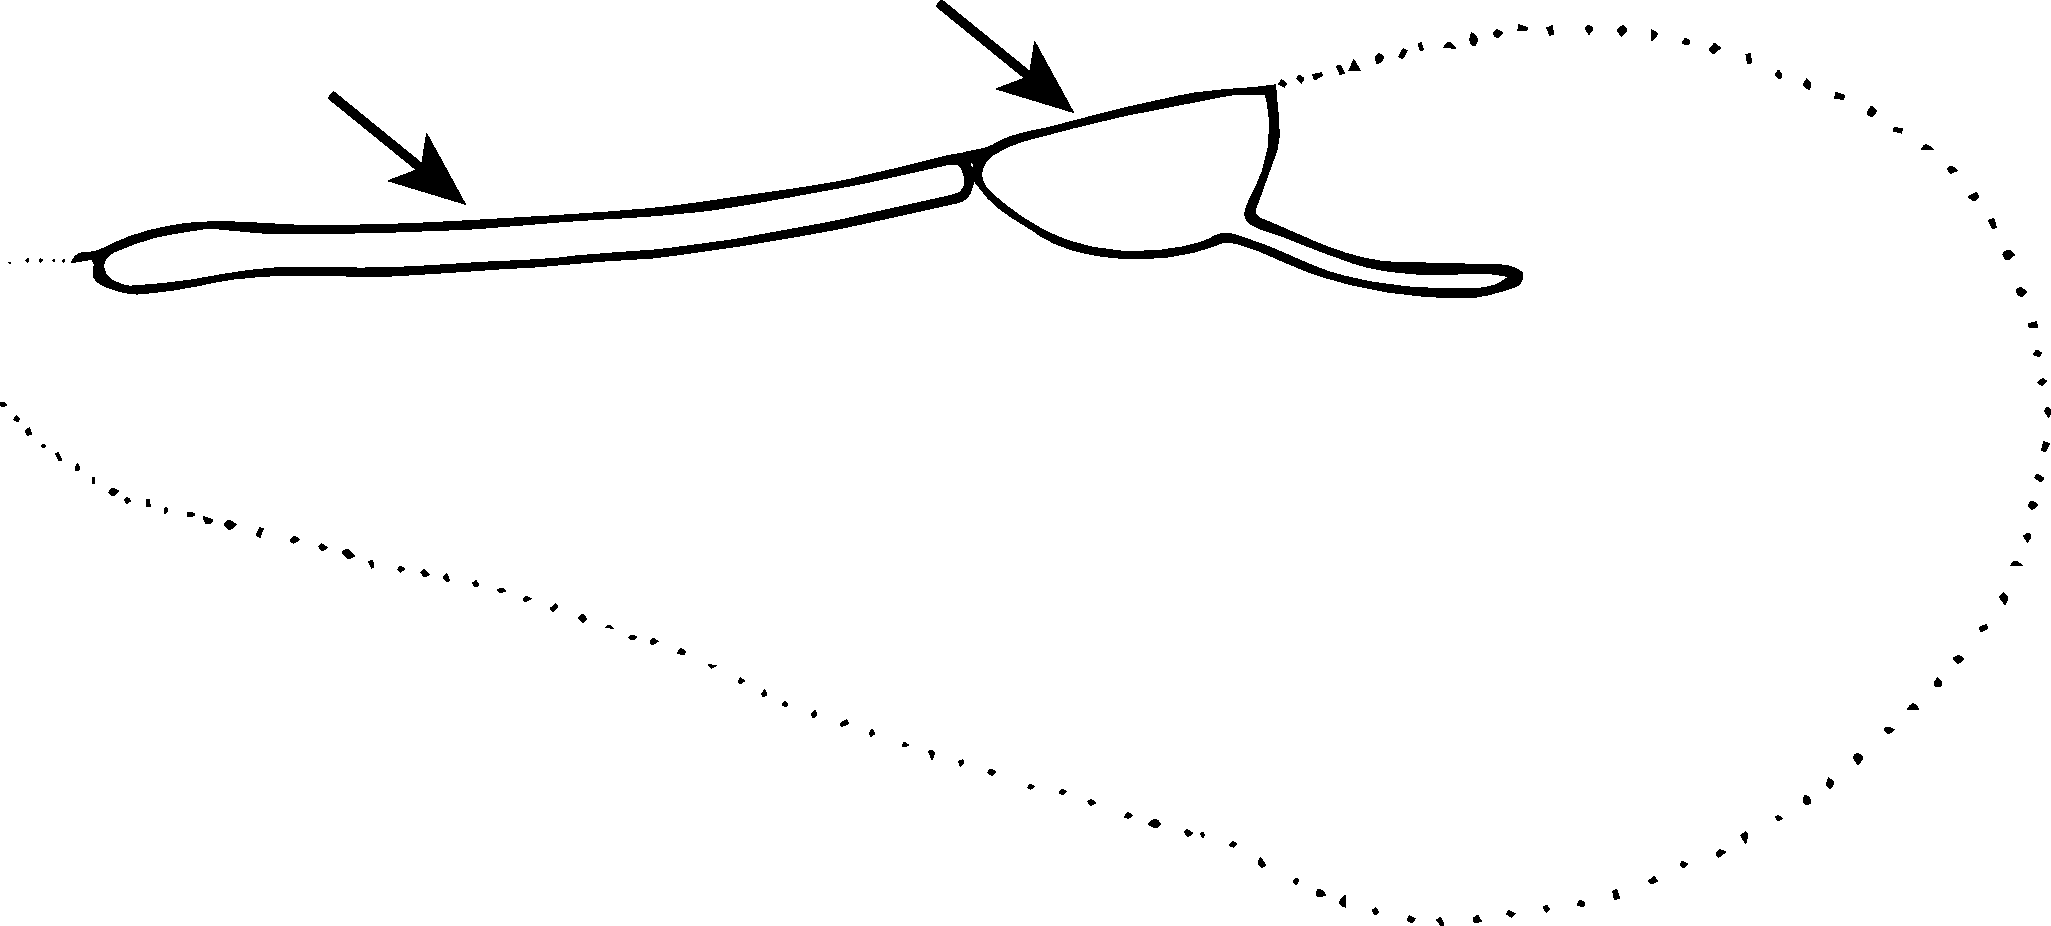
\includegraphics[width=\textwidth]{hymenoptera/MegaspilidWing}
  \caption{}
  \label{fig:megaspilid1}
\end{subfigure}
    \hfill
\begin{subfigure}[ht!]{0.38\textwidth}
    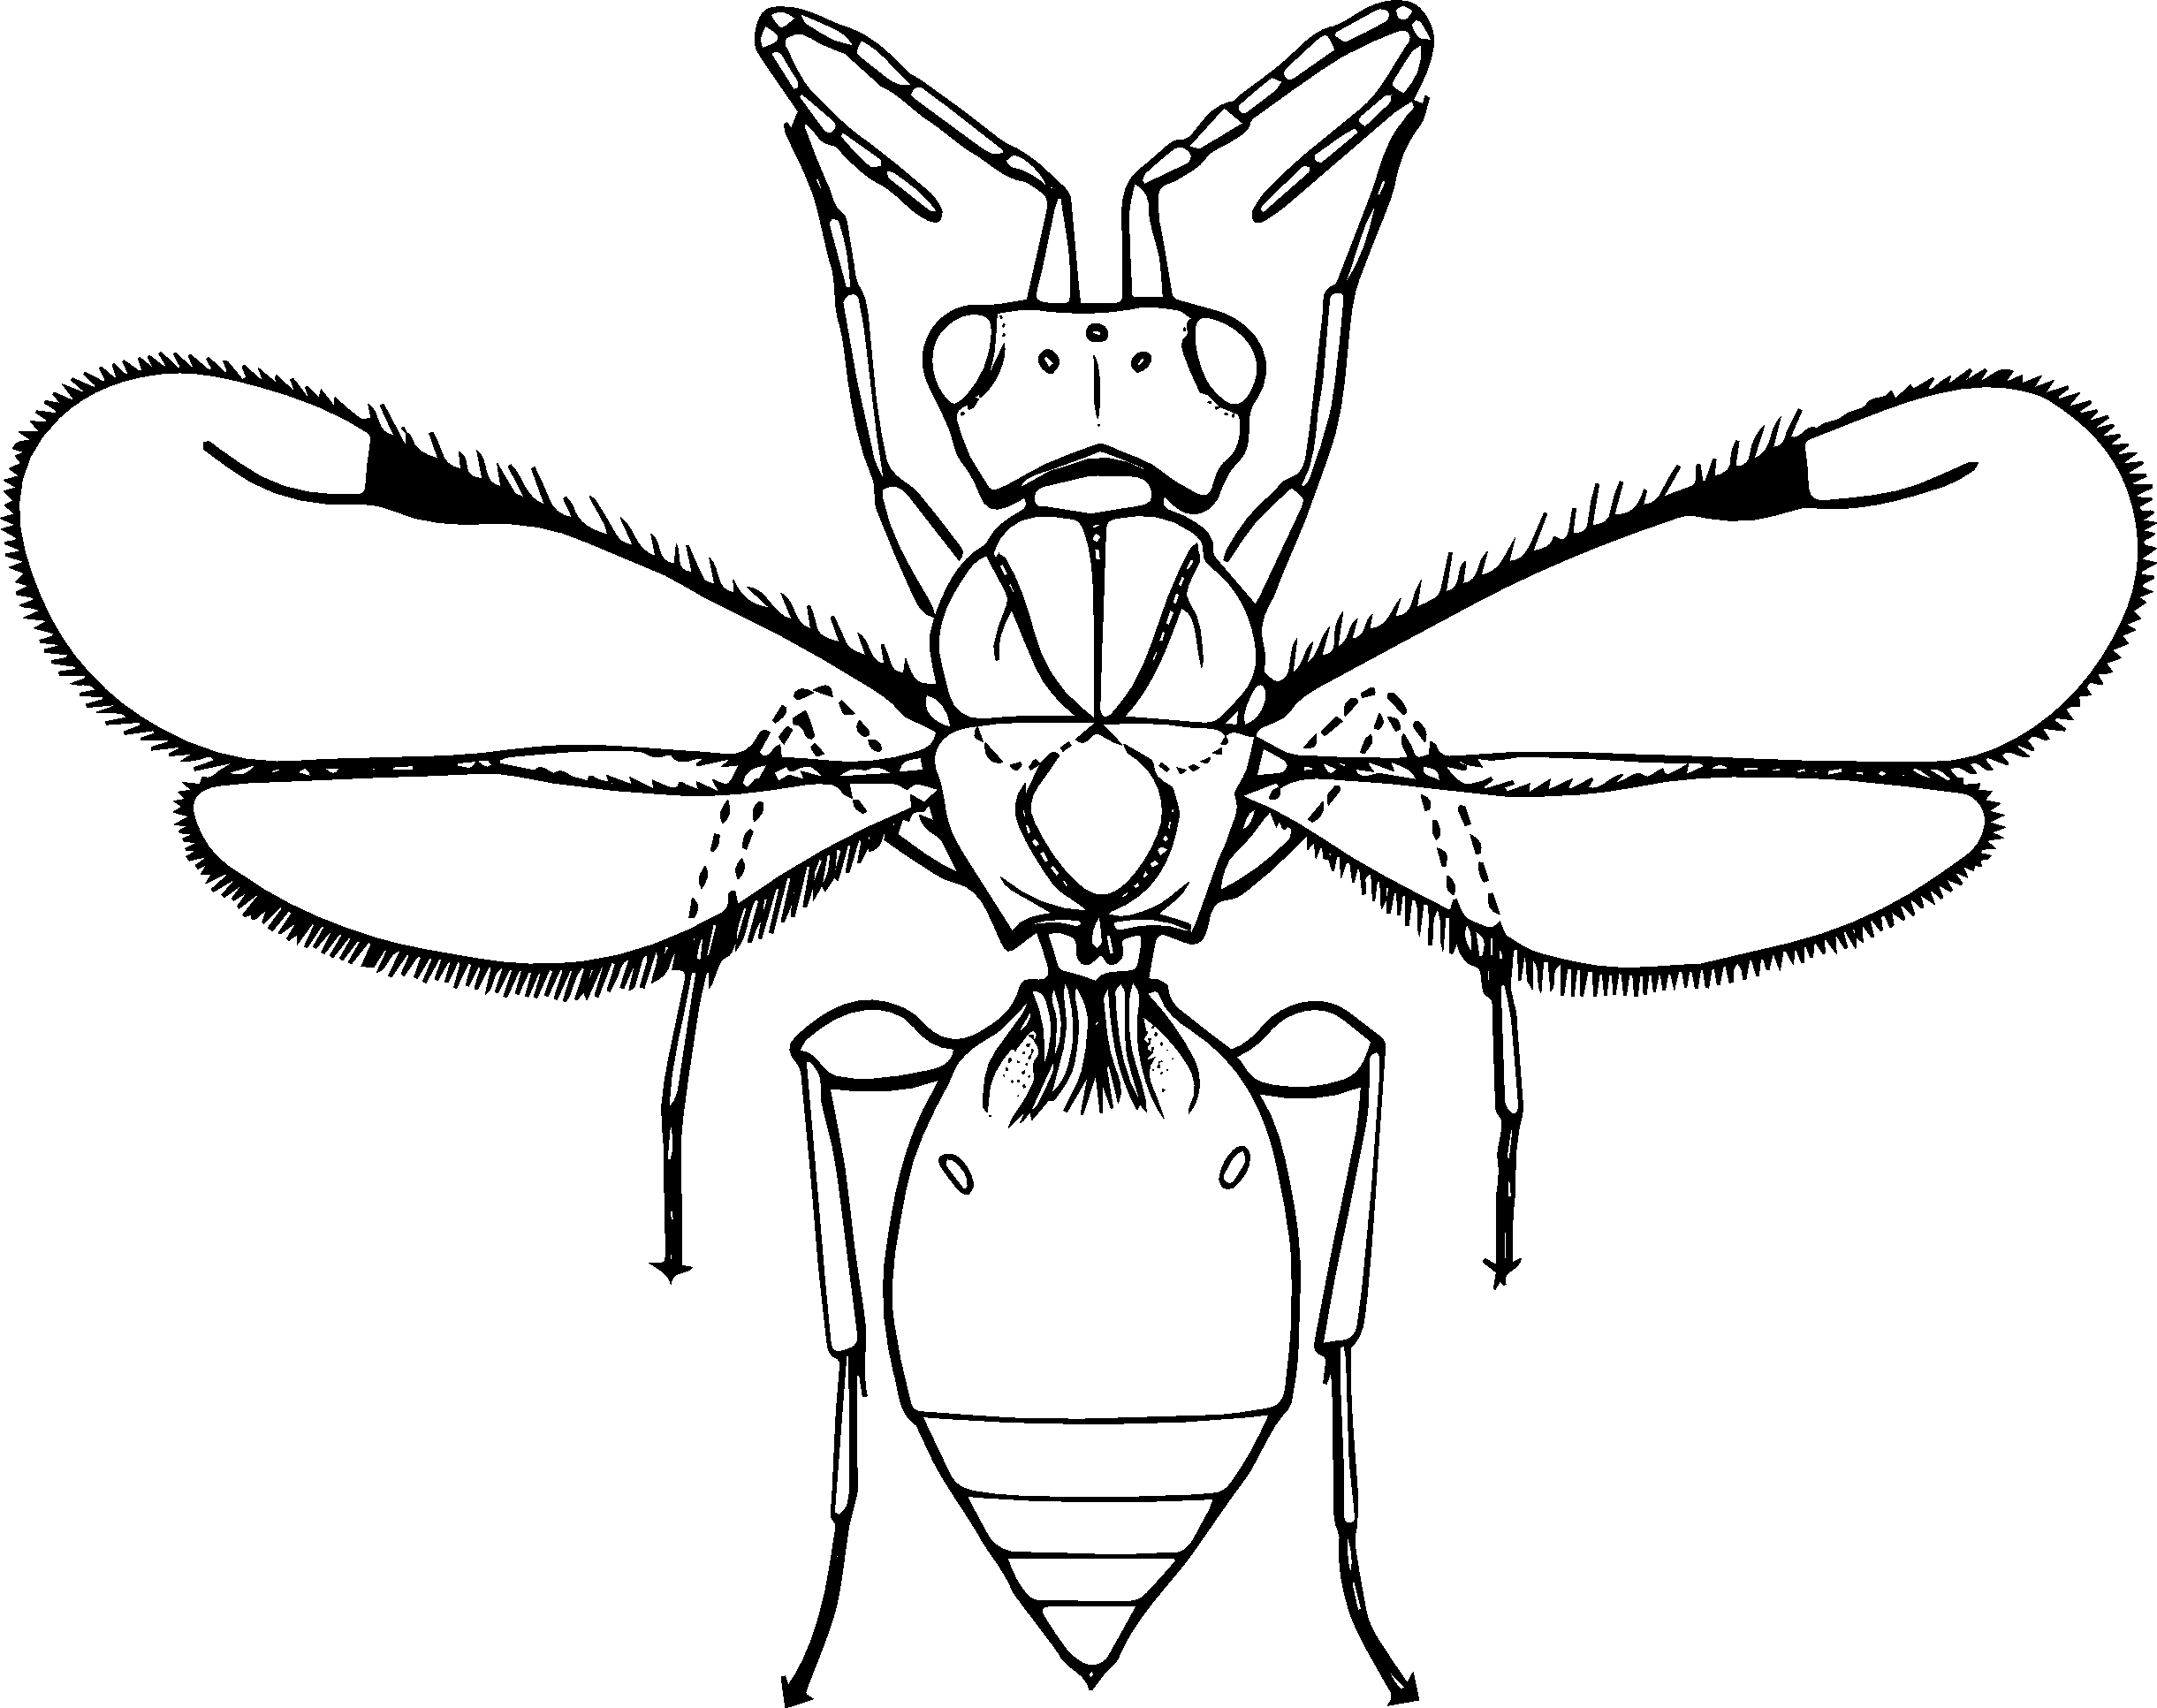
\includegraphics[width=\textwidth]{hymenoptera/MegaspilidHabitus}
  \caption{}
  \label{fig:megaspilid2}
\end{subfigure}
    \caption{Megaspilidae. \textbf{(a)} Fore wing \citep[][pg. 566]{goulet1993hymenoptera}; \textbf{(b)} dorsal habitus \citep[][Fig. 209]{goulet1993hymenoptera}}\label{fig:megaspilid}
\end{figure}

\subsubsection{Braconidae}\index{Braconidae}
\noindent{}\textit{Diagnostic characters:} Antenna usually with 16 or more antennomeres (figure \ref{fig:braconid1}); fore wing C + Sc + R fused (\textit{i.e.}, anterior margin of wing with relatively thick wing vein); pterostigma usually present; one recurrent vein or none (figure \ref{fig:braconid2}); no ``horse head'' cell (compare with Ichneumonidae); first and second metasomal segments often fused and immobile dorsally.\vspace{3mm}

\noindent{}\textit{Natural history:} These parasitoid wasps are extraordinarily diverse, with almost 20,000 described species. Many of them, especially the subfamily Microgastrinae, coevolved with viruses (polydnaviruses), which help them overcome the hosts' immune response.

\begin{figure}[ht!]
    \centering
    \begin{subfigure}[ht!]{0.45\textwidth}
        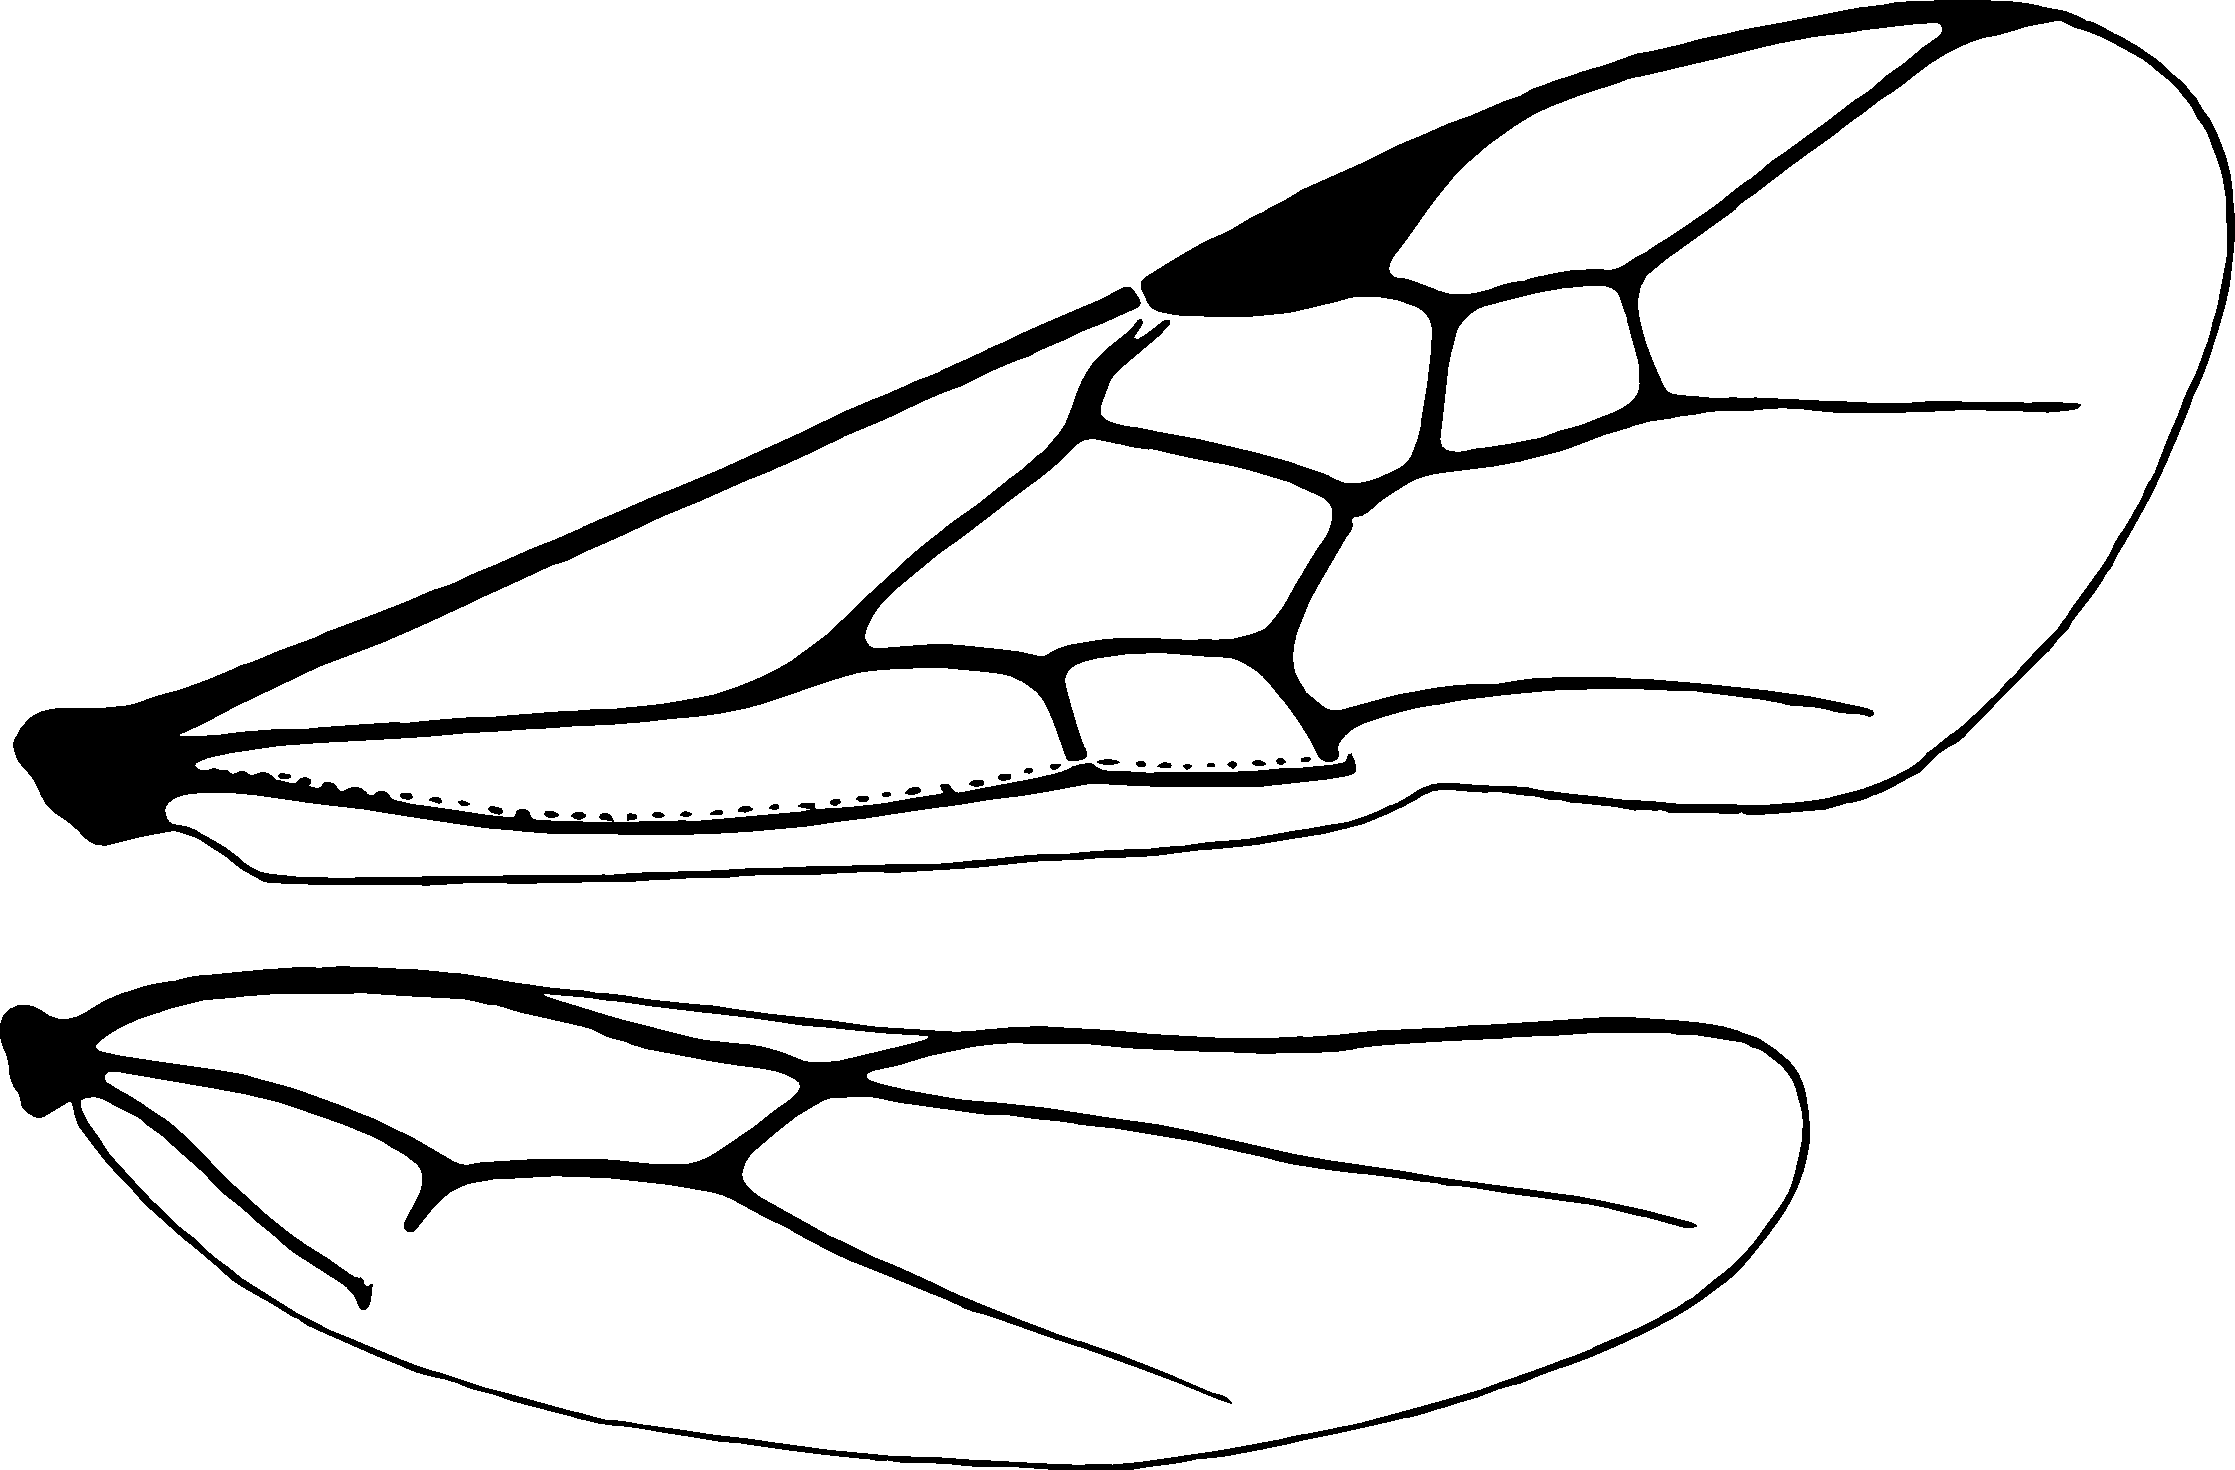
\includegraphics[width=\textwidth]{hymenoptera/braconidWings}
        \caption{}
        \label{fig:braconid1}
    \end{subfigure}
    \hfill
    \begin{subfigure}[ht!]{0.34\textwidth}
        \reflectbox{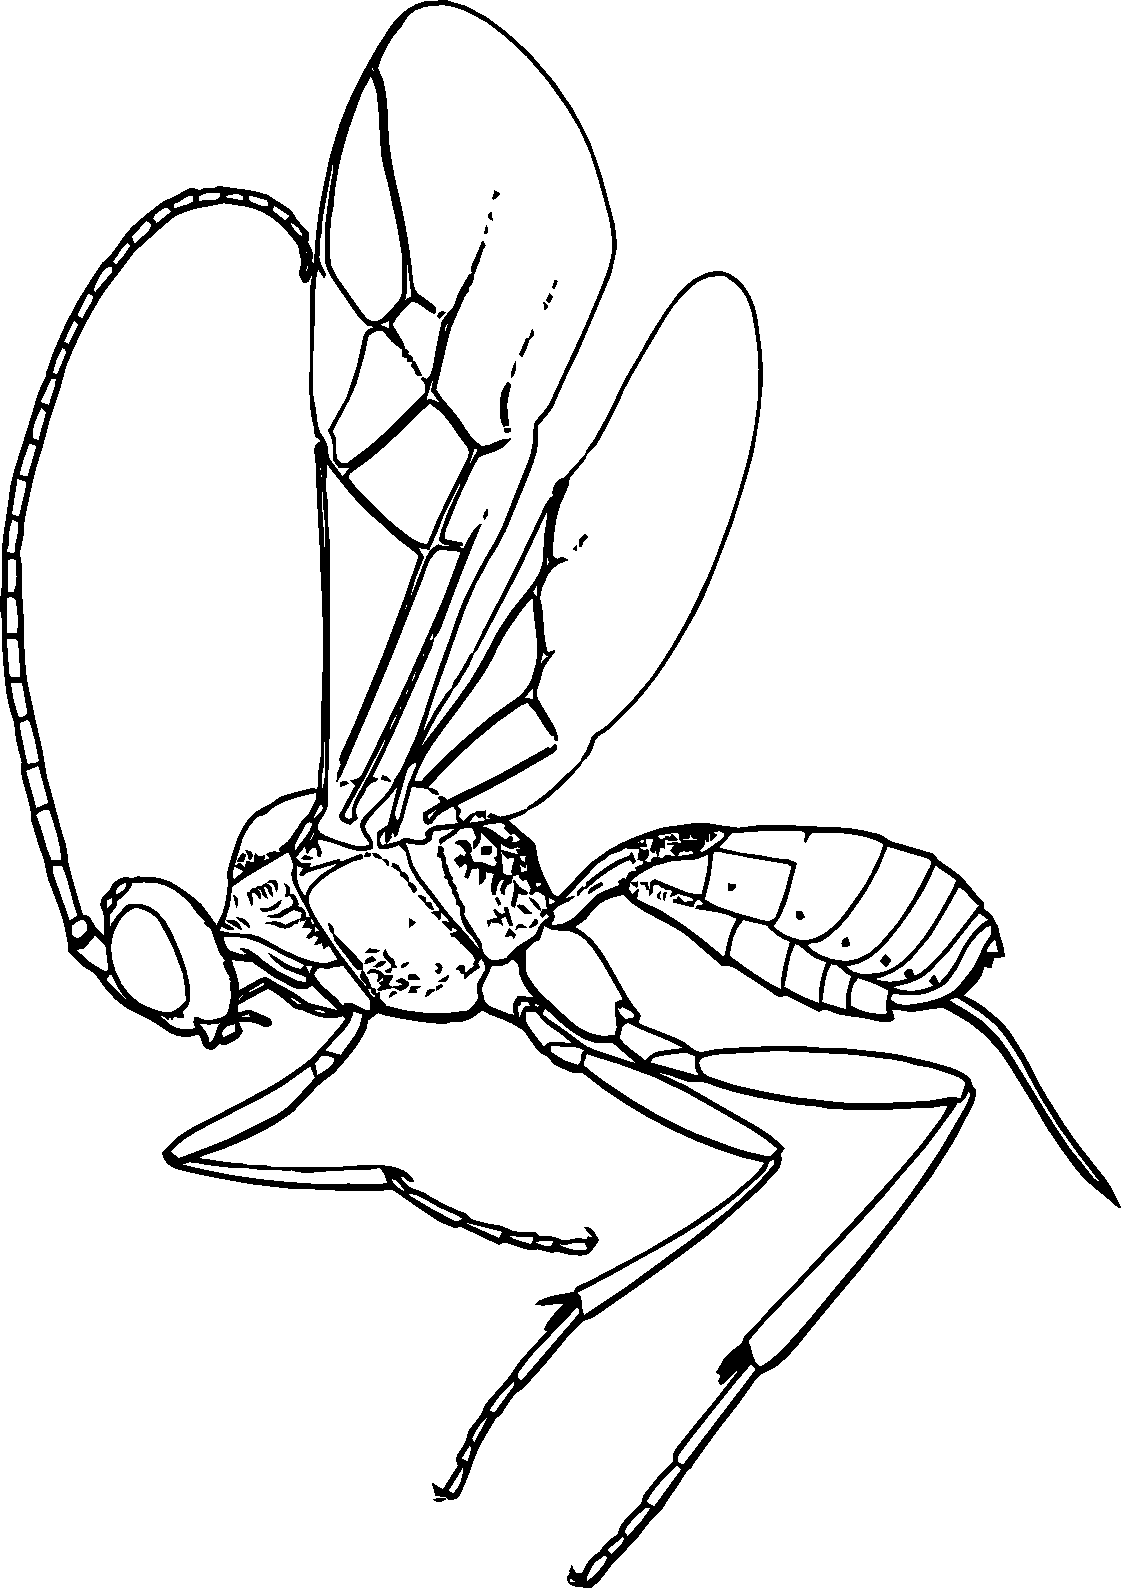
\includegraphics[width=\textwidth]{hymenoptera/BraconidHabitus}}
        \caption{}
        \label{fig:braconid2}
    \end{subfigure}
    \caption{Braconidae. \textbf{(a)} Wings \citep[redrawn from][Fig. 56]{comstock1918wings}; \textbf{(b)} lateral habitus \citep[][Fig. 138]{goulet1993hymenoptera}}\label{fig:braconids}
\end{figure}

\subsubsection{Ichneumonidae (ichneumon wasps)}\index{Ichneumonidae}
\noindent{}\textit{Diagnostic characters:} Antenna usually with 16 or more antennomeres; fore wing C + Sc + R fused (\textit{i.e.}, anterior margin of wing with relatively thick wing vein); pterostigma usually present; two recurrent veins present (figure \ref{fig:ichneumonid1} arrow); ``horse head cell'' present (often not quite horse-like); first and second metasomal segments not fused.\vspace{3mm}

\noindent{}\textit{Natural history:} One of the most diverse families of insects, with at least 24,000 named species and many, many more remaining to be described. Like their sister family, Braconidae, some species inject polydnaviruses into the hosts, along with the egg(s), to combat the hosts' immune responses. These wasps are parasitoids of many kinds of arthropods but mostly other insects.

\begin{figure}[ht!]
    \centering
    \begin{subfigure}[ht!]{0.45\textwidth}
        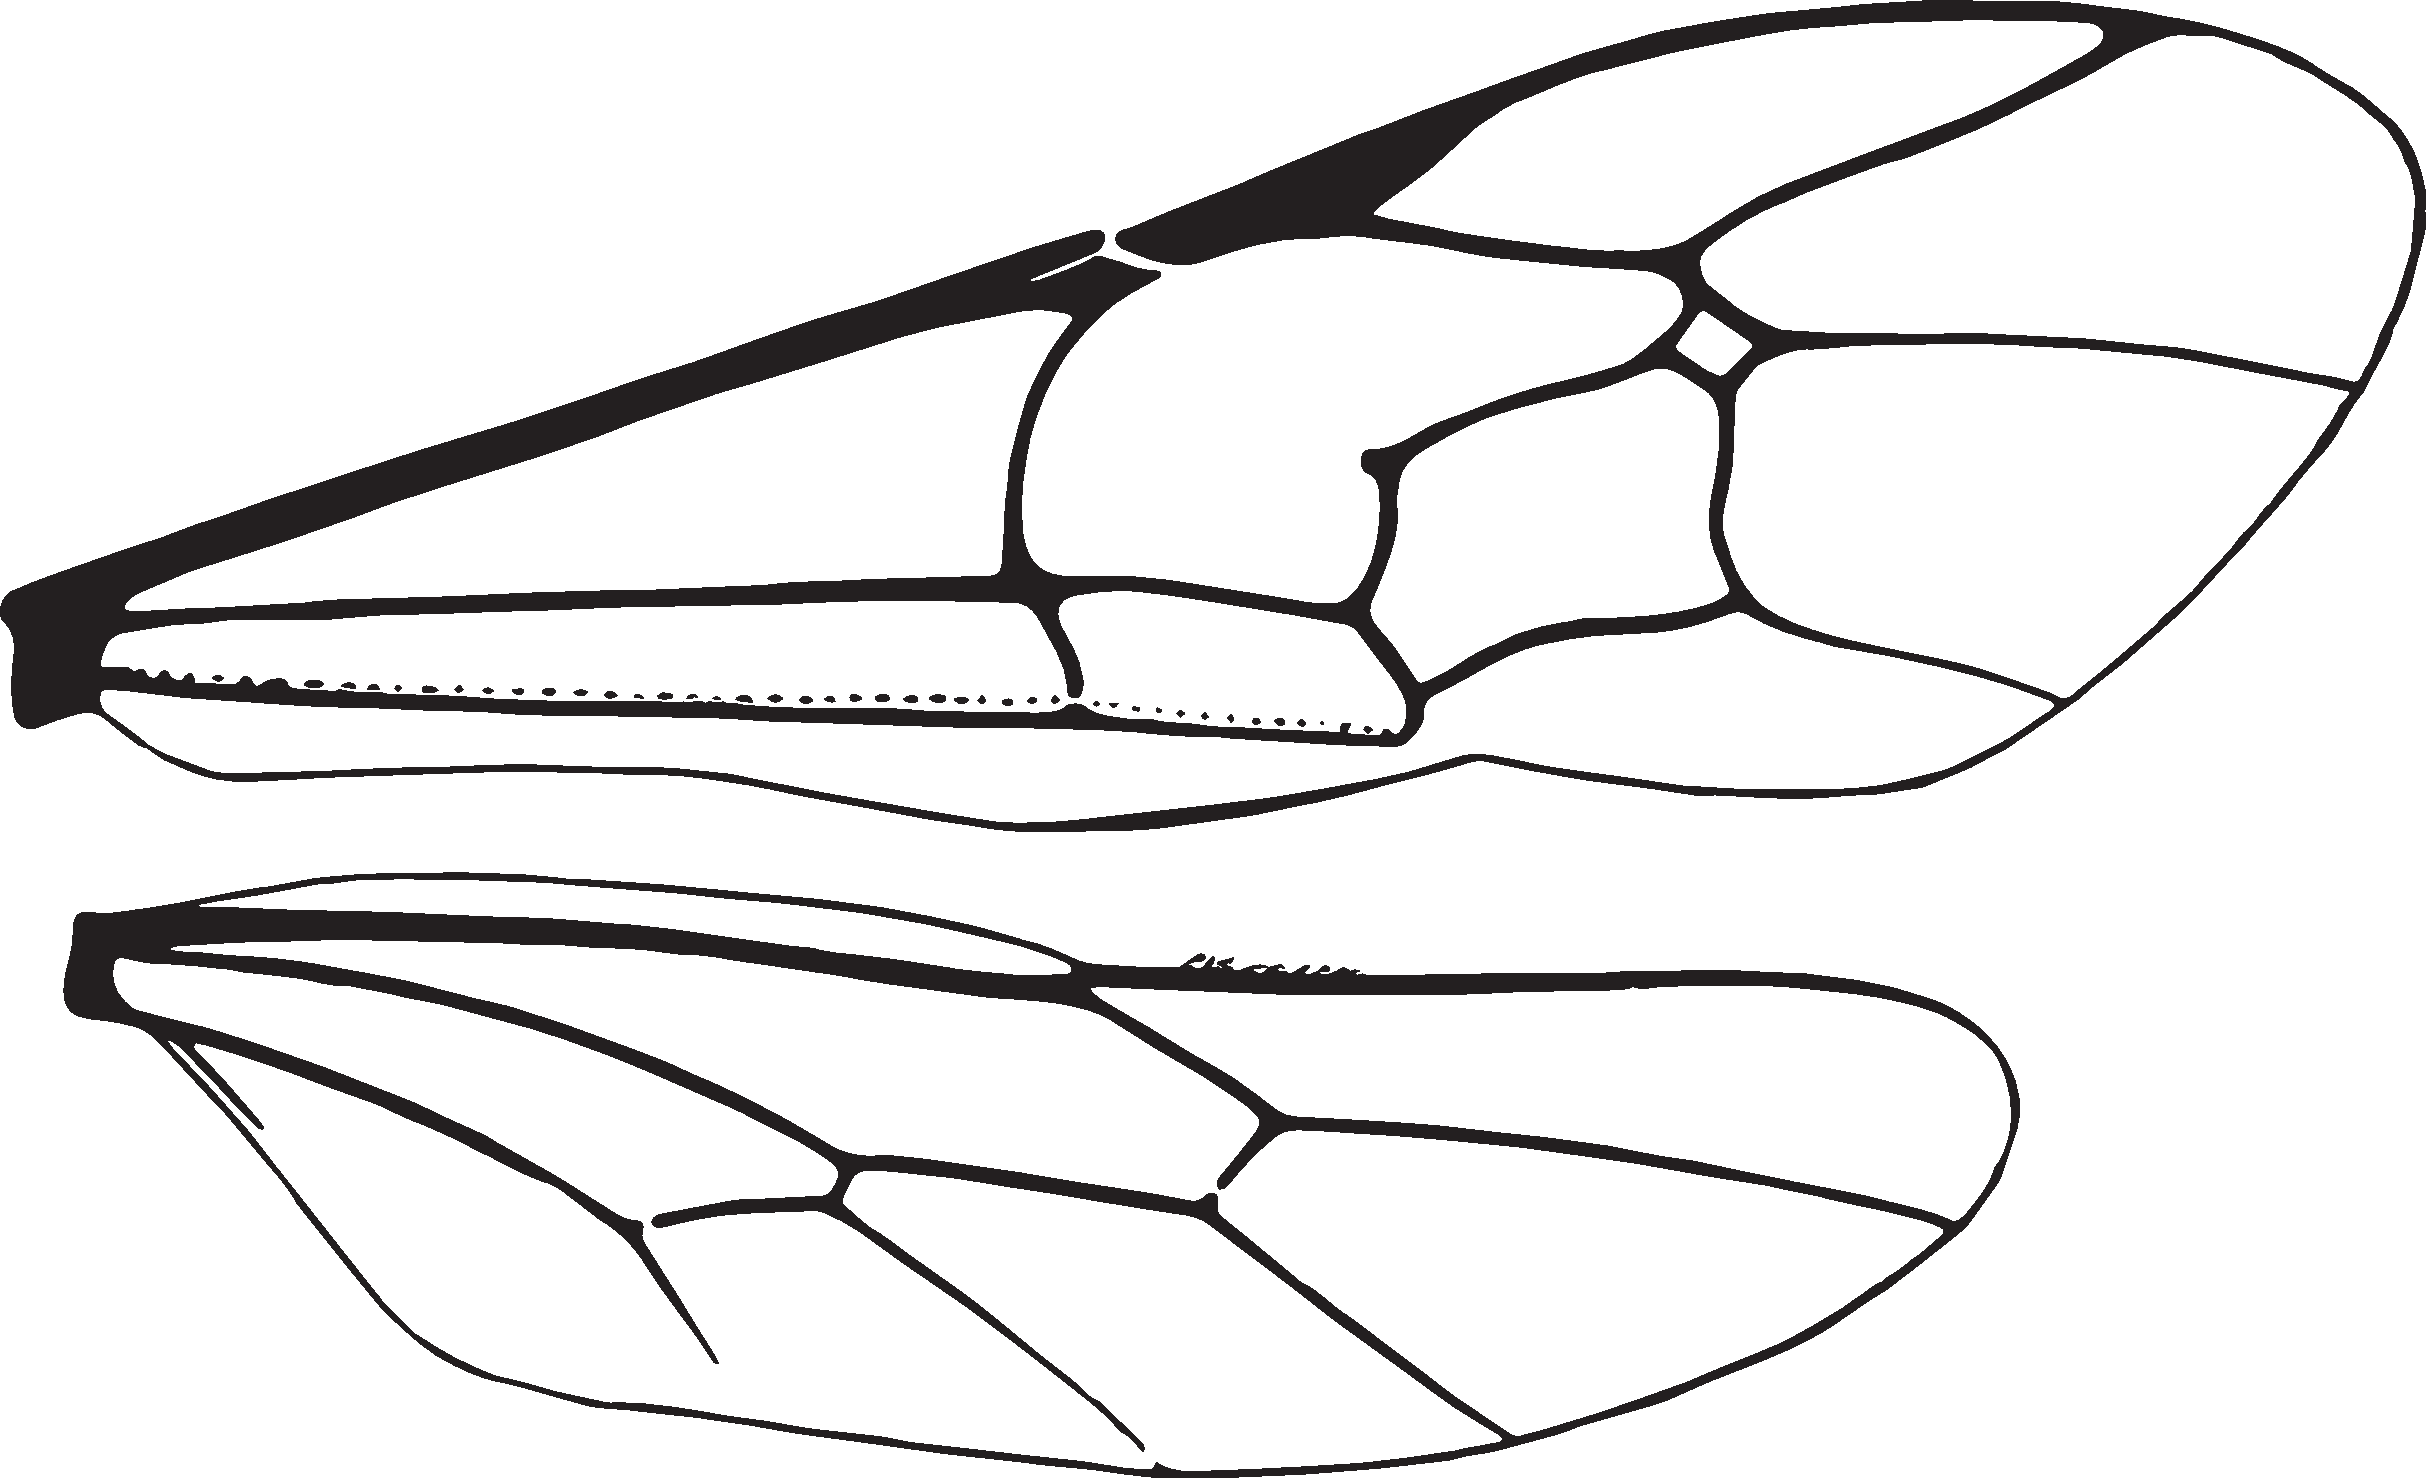
\includegraphics[width=\textwidth]{hymenoptera/ichneumonidWings}
        \caption{}
        \label{fig:ichneumonid1}
    \end{subfigure}
    \hfill
    \begin{subfigure}[ht!]{0.4\textwidth}
        \reflectbox{\includegraphics[width=\textwidth]{hymenoptera/IchneumonidHabitus}}
        \caption{}
        \label{fig:ichneumonid2}
    \end{subfigure}
    \caption{Ichneumonidae. \textbf{(a)} Wings \citep[redrawn from][Fig. 55]{comstock1918wings}; \textbf{(b)} lateral habitus \citep[][Fig. 159]{goulet1993hymenoptera}}\label{fig:ichneumonids}
\end{figure}

\subsubsection{Pelecinidae}\index{Pelecinidae}
\noindent{}\textit{Diagnostic characters:} relatively large (20--70 mm long); fore wing with one cell enclosed by tubular veins; petiole tubular, female abdominal segments elongate, tubular (figure \ref{fig:pelecinid1}).\vspace{3mm}

\noindent{}\textit{Natural history:} There is only one extant species, whose distribution spans from Canada to Argentina. Females use their extended metasomas to probe soil for hosts, which are larval scarab beetles (\textit{Phyllophaga} spp.)

\begin{figure}[ht!]
  \centering
    \reflectbox{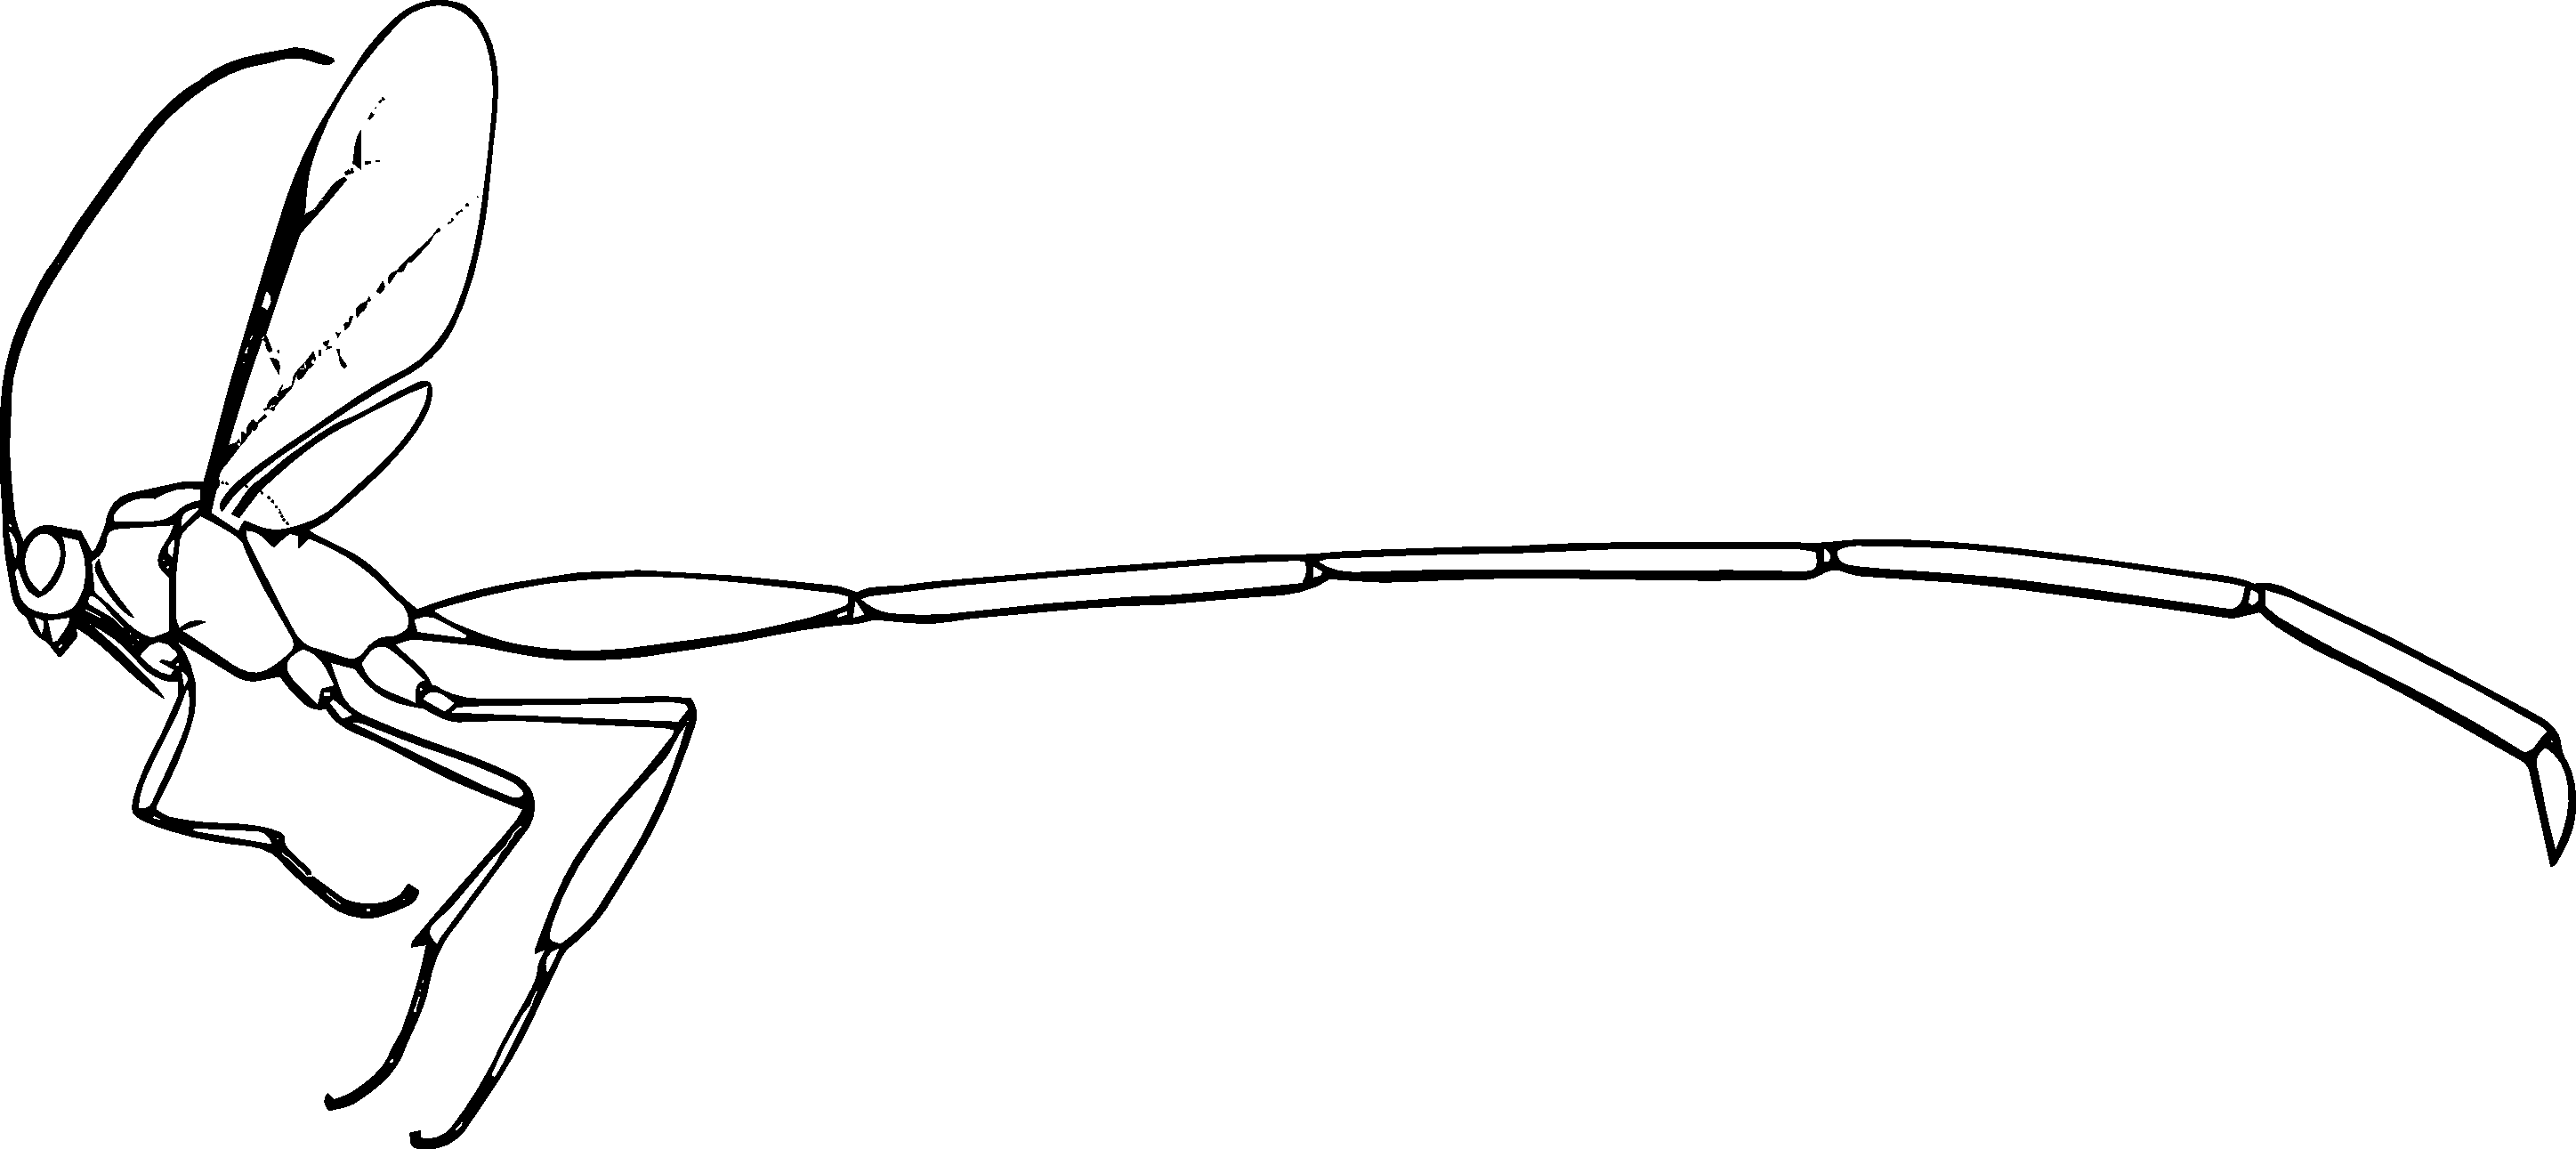
\includegraphics[width=0.8\textwidth]{hymenoptera/PelecinidHabitus}}
  \caption{Pelecinidae, female habitus \citep[][Fig. 198]{goulet1993hymenoptera}}
  \label{fig:pelecinid1}
\end{figure}

\subsubsection{Diapriidae}\index{Diapriidae}
\noindent{}\textit{Diagnostic characters:} Antenna elbowed; antennal shelf present, articulation dorsally distant from clypeus; antenna with 11--15 antennomeres; fore wing venation variable (sometimes lacking wing cells); usually black or brown, often shiny and smooth in parts; petiole tubular.\vspace{3mm}

\noindent{}\textit{Natural history:} Approximately 2,500 species have been described from around the world. These wasps are very frequently collected in yellow pans and leaf litter samples, and most species are understood to be parasitoids of larval dipterans.

\begin{figure}[ht!]
  \centering
    \reflectbox{\includegraphics[width=0.55\textwidth]{hymenoptera/DiapriidHabitus}}
  \caption{Diapriidae habitus \citep[][Fig. 206]{goulet1993hymenoptera}}
  \label{fig:diapriid1}
\end{figure}

\subsubsection{Scelionidae}\index{Scelionidae}
\noindent{}\textit{Diagnostic characters:} Antenna elbowed; antennal shelf absent; antennal sockets usually close to clypeus; fore wing with 3 veins, pterostigma absent (figure \ref{fig:scelionid1}); fore wing without proximal tubular vein on anterior margin; antenna usually with 11--12 antennomeres; small to very small, usually black or brown; pronotum adjacent to tegula; petiole not tubular; abdomen often flat, with sharp lateral edges.\vspace{3mm}

\noindent{}\textit{Natural history:} More than 3,000 species have been described from around the world. These wasps are parasitoids of insect eggs, and several species have been recruited for biocontrol.\vspace{3mm}

\begin{theo}
{}What do you notice about scelionid body shapes? What do you think is their biological significance?
\end{theo}

\begin{figure}[ht!]
  \centering
\begin{subfigure}[ht!]{0.5\textwidth}
    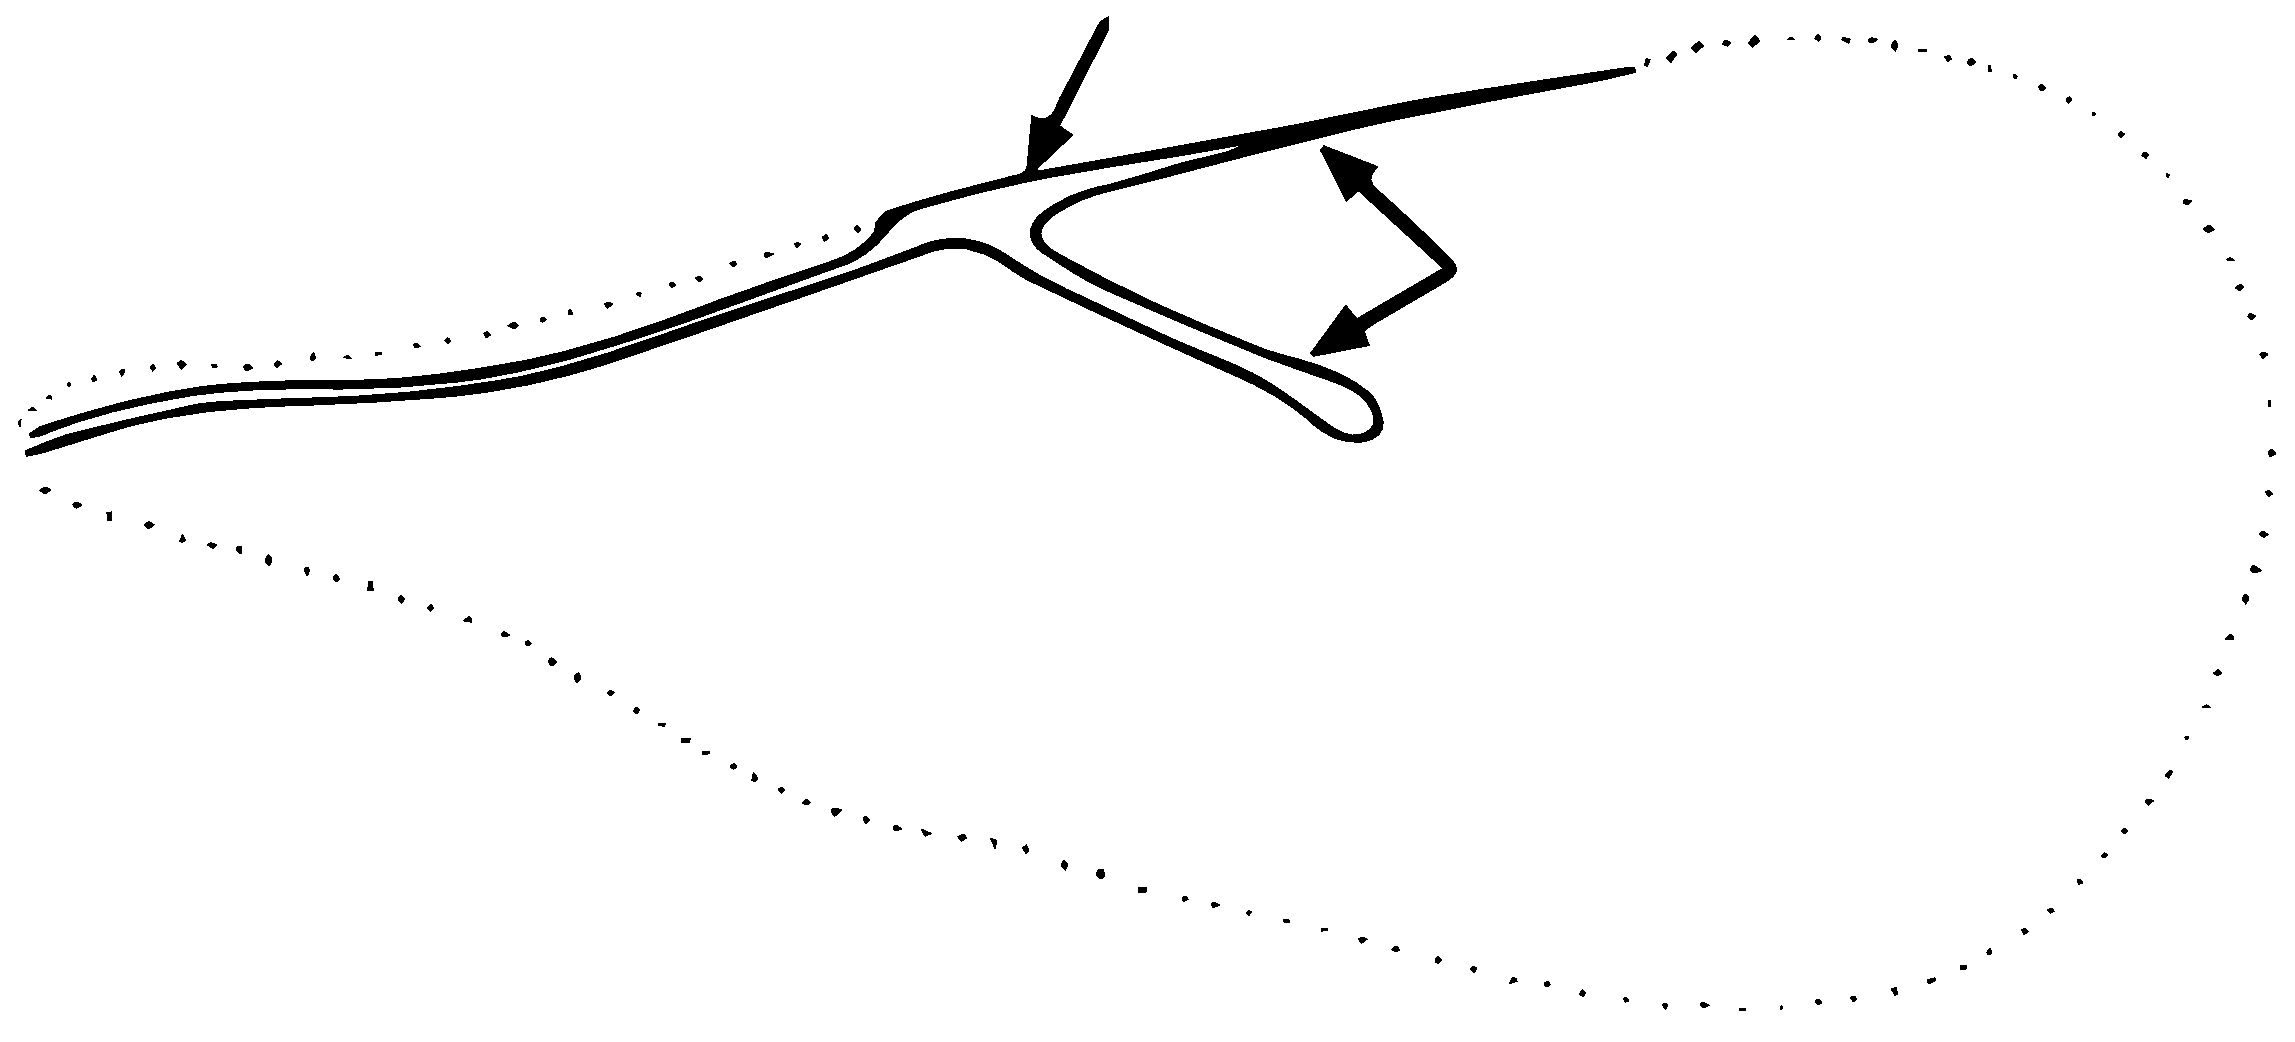
\includegraphics[width=\textwidth]{hymenoptera/ScelionidWing}
  \caption{}
  \label{fig:scelionid1}
\end{subfigure}
    \hfill
\begin{subfigure}[ht!]{0.4\textwidth}
    \reflectbox{\includegraphics[width=\textwidth]{hymenoptera/ScelionidHabitus}}
  \caption{}
  \label{fig:scelionid2}
\end{subfigure}
    \caption{Scelionidae. \textbf{(a)} Fore wing \citep[][pg. 560]{goulet1993hymenoptera}; \textbf{(b)} lateral habitus \citep[][Fig. 207]{goulet1993hymenoptera}}\label{fig:scelionids}
\end{figure}

\paragraph*{Cynipoidea} The next two families are classified in Cynipoidea, which all share the following characteristics:\index{Cynipoidea}
\begin{itemize}
\item distinctive wing venation: no proximal vein along anterior margin, with well developed marginal cell (R1), no pterostigma
\item antenna with 11--16 antennomeres, not elbowed (\textit{i.e}., not geniculate)
\item abdomen laterally flattened
\end{itemize}

\subsubsection{Figitidae}\index{Figitidae}
\noindent{}\textit{Diagnostic characters:} fore wing with cell RI 3--4 times as long as wide; hind leg with tarsomere 1 not longer than remaining tarsomeres combined; petiole of metasoma usually elongate, longer than wide; scutellum usually elaborate, with keel-like structure or cup-like process; if scutellum not elaborate, then 3 abdominal tergites visible or head wider than mesosoma.\vspace{3mm}

\noindent{}\textit{Natural history:} There are $\sim$1,400 described species, the vast majority of which are parasitoids of Diptera larvae. Some species are hyperparasitoids on Sternorrhyncha.\vspace{3mm}

\begin{figure}[ht!]
  \centering
\begin{subfigure}[ht!]{0.45\textwidth}
\reflectbox{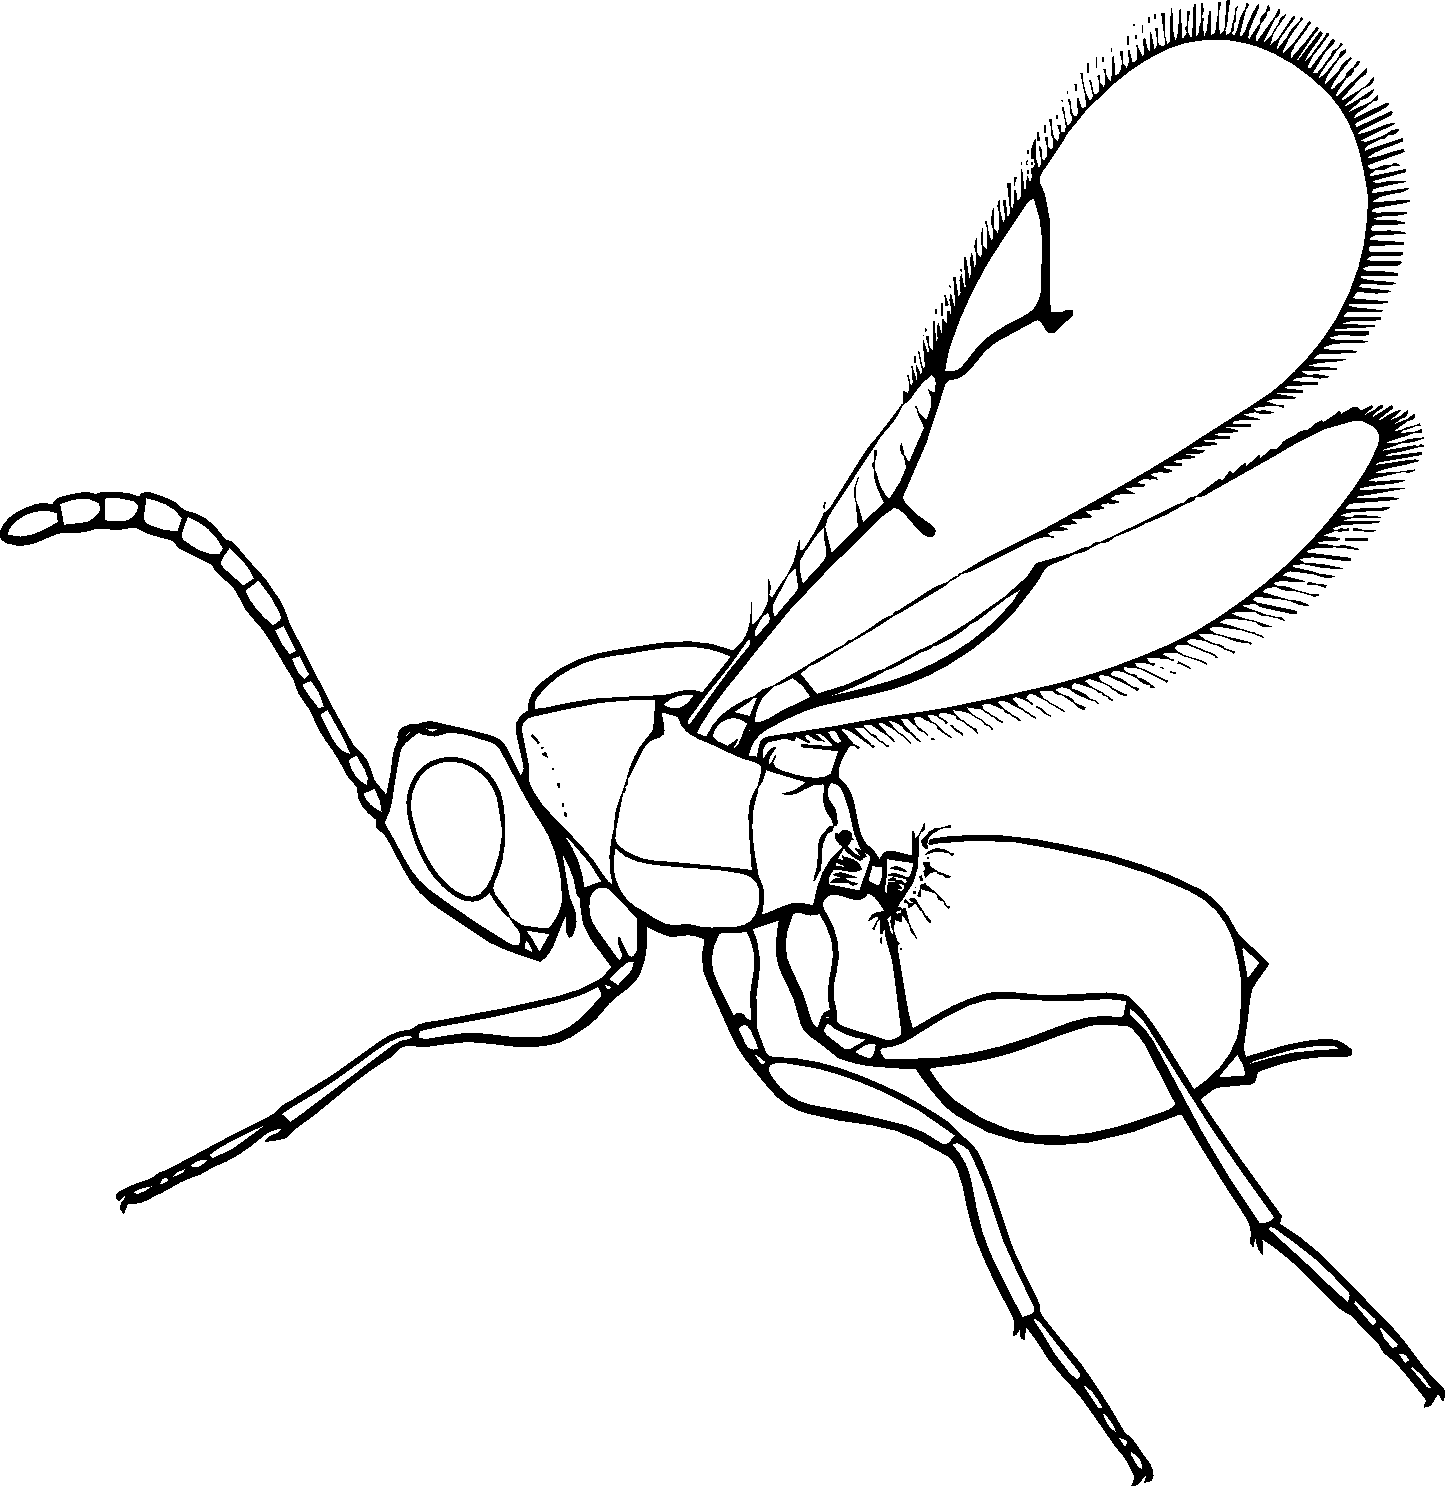
\includegraphics[width=\textwidth]{hymenoptera/FigitidHabitus}}
  \caption{Figitidae}
  \label{fig:figid1}
\end{subfigure}
    \hfill
\begin{subfigure}[ht!]{0.4\textwidth}
\reflectbox{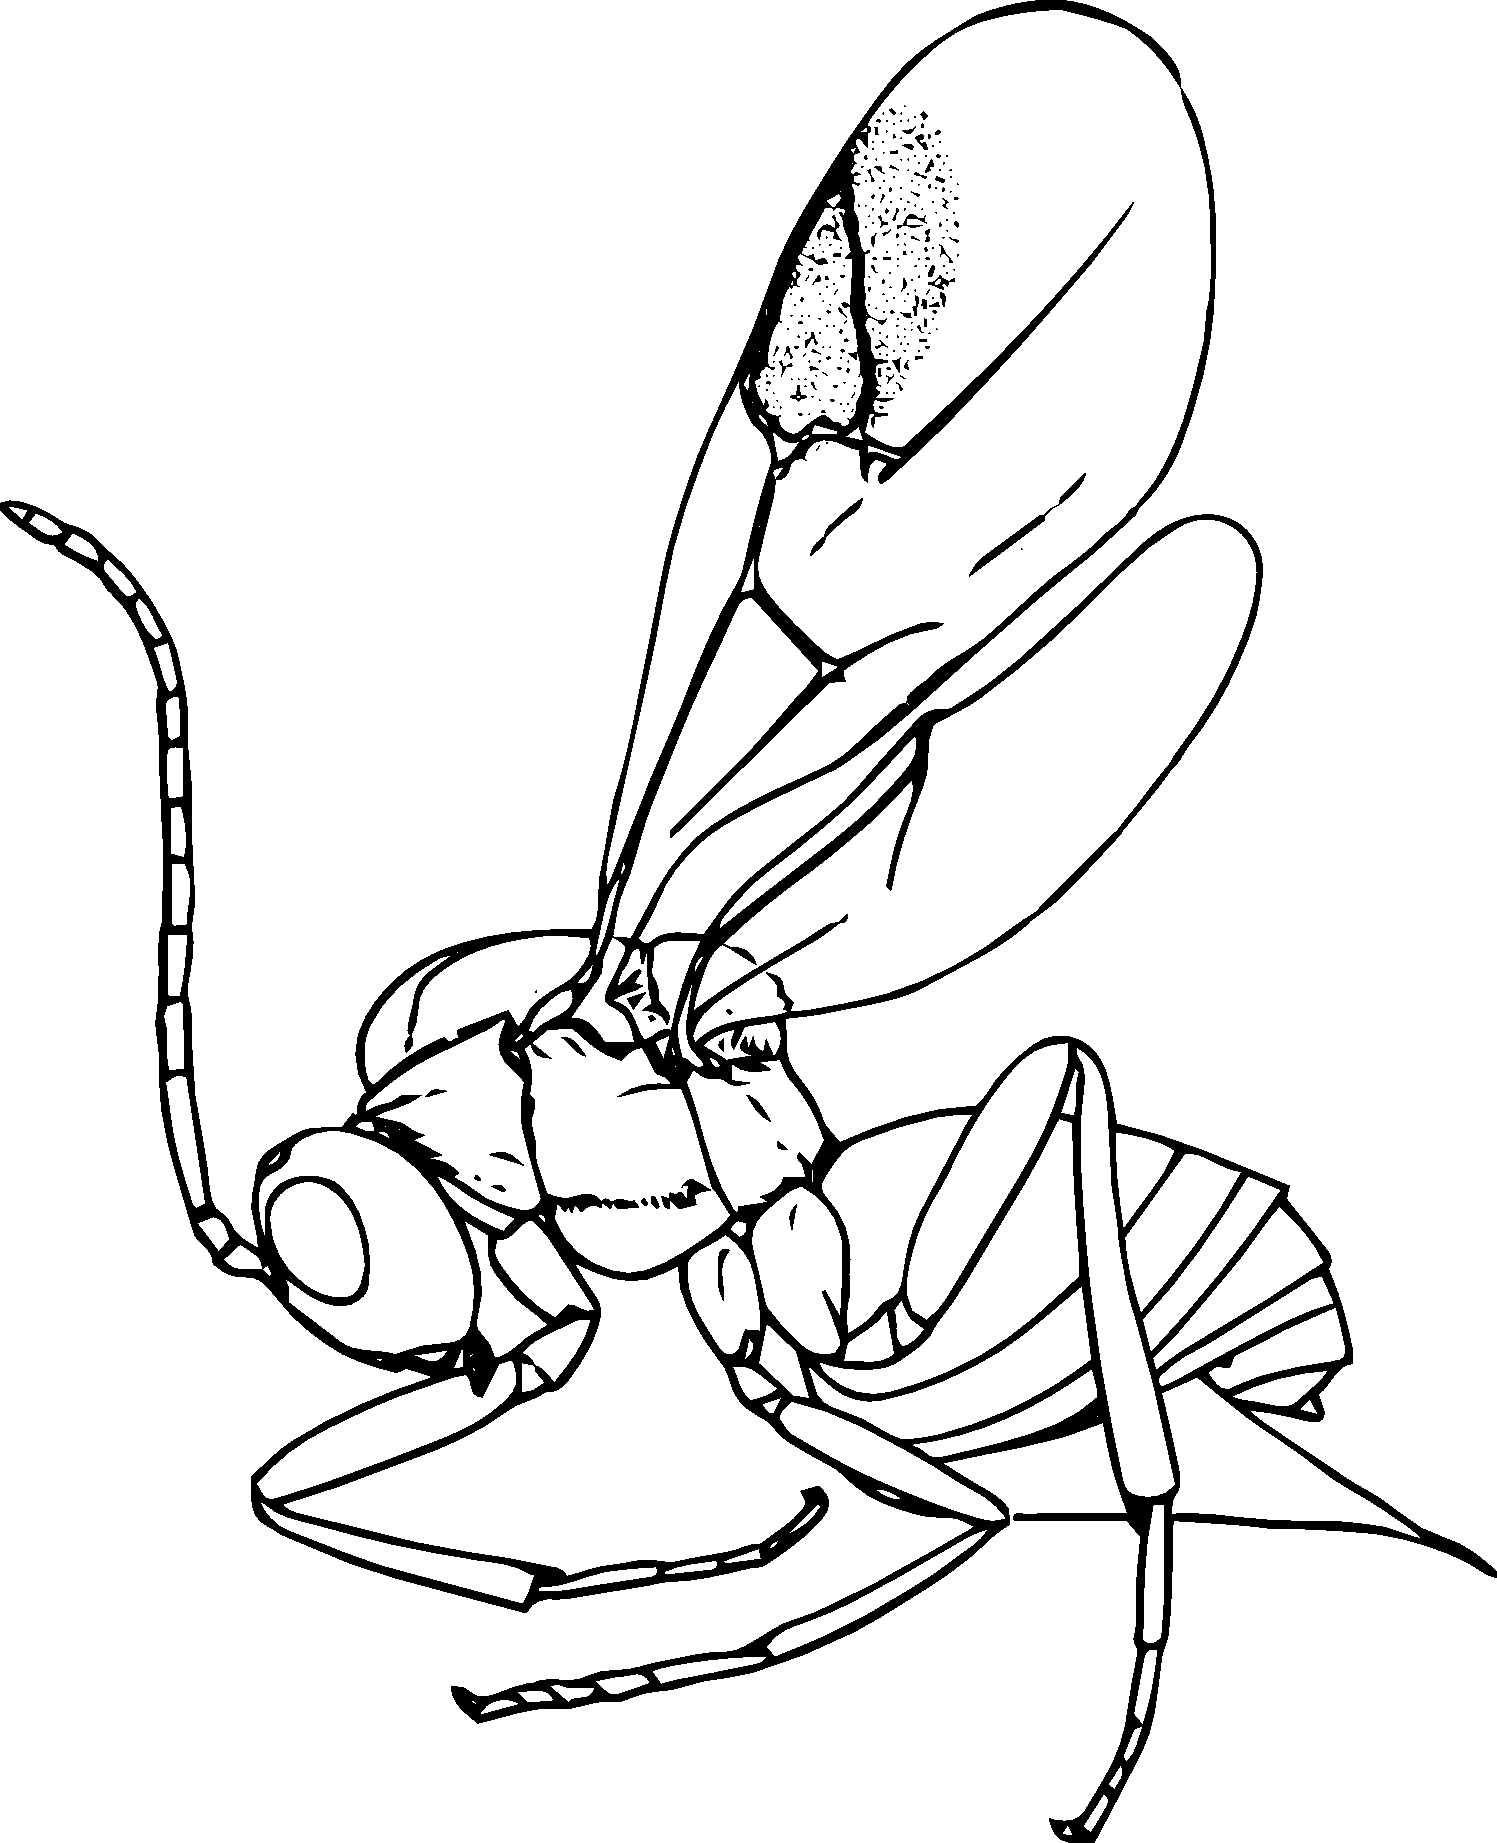
\includegraphics[width=\textwidth]{hymenoptera/CynipidHabitus}}
  \caption{Cynipidae}
  \label{fig:cynipid1}
\end{subfigure}
    \caption{Cynipoidea. \textbf{(a)} Figitidae habitus \citep[][Fig. 195]{goulet1993hymenoptera}; \textbf{(b)} Cynipidae habitus \citep[][Fig. 197]{goulet1993hymenoptera}}\label{fig:cynipoids}
\end{figure}

\subsubsection{Cynipidae (gall wasps)}\index{Cynipidae}
\noindent{}\textit{Diagnostic characters:} fore wing with cell RI 3--4 times as long as wide; hind leg with tarsomere 1 not longer than remaining tarsomeres combined; petiole of metasoma hidden or wider than long (figure \ref{fig:cynipid1}); scutellum rounded, not elaborate but usually with rough texture; \textgreater{}3 abdominal tergites visible, head always wider than mesosoma.\vspace{3mm}

\noindent{}\textit{Natural history:} Most of the $\sim$1,300 species are gall-makers on plants or inquilines inside the galls of other insects. Many of these wasps are associated with oaks (\textit{Quercus} spp.). This family will likely be split into multiple families soon.\vspace{3mm}

\begin{theo}
{}Based on what you know about plants, which may be very little, how do you think gall wasps can induce galls and facilitate predictable extended phenotypes?
\end{theo}\vspace{3mm}

\paragraph*{Chalcidoidea} The next families are classified in the super diverse taxon Chalcidoidea. We'll look at five families, but keep in mind there are more than 50(!) chalcidoid families worldwide, many of which are quite common in the eastern USA. They all share the following characteristics, the combination of which separates chalcidoids from other apocritans:\index{Chalcidoidea}
\begin{itemize}
\item antenna geniculate, with ``ring segments'' (\textit{i.e.}, short, ring-like sclerites at the base of the flagellum)
\item pronotum not reaching tegula (\textit{i.e.}, a sclerite (prepectus) is present between the pronotum and tegula)
\item fore wing with 3 veins, similar to Scelionidae
\end{itemize}

\subsubsection{Chalcididae}\index{Chalcididae}
\noindent{}\textit{Diagnostic characters:} Tarsi 5-segmented; hind femora greatly swollen and often toothed, hind tibiae curved to fit femora (figure \ref{fig:chalcidid}); hind coxae much larger than front coxae (figure \ref{fig:chalcidid}); fairly large (for chalcidoids!); very rarely (if ever) metallic in color.\vspace{3mm}

\noindent{}\textit{Natural history:} Almost 1,500 species are known worldwide. Most are parasitoids of Lepidoptera (especially the pupa) or late instar Diptera.\vspace{3mm}

\begin{theo}
{}What do you think is/are the function(s) of the hind femora in Chalcididae? What makes them so large?
\end{theo}

\begin{figure}[ht!]
  \centering
\begin{subfigure}[ht!]{0.45\textwidth}
    \reflectbox{\includegraphics[width=\textwidth]{hymenoptera/ChalcididHabitus}}
  \caption{Chalcididae}
  \label{fig:chalcidid}
\end{subfigure}
    \hfill
\begin{subfigure}[ht!]{0.45\textwidth}
    \reflectbox{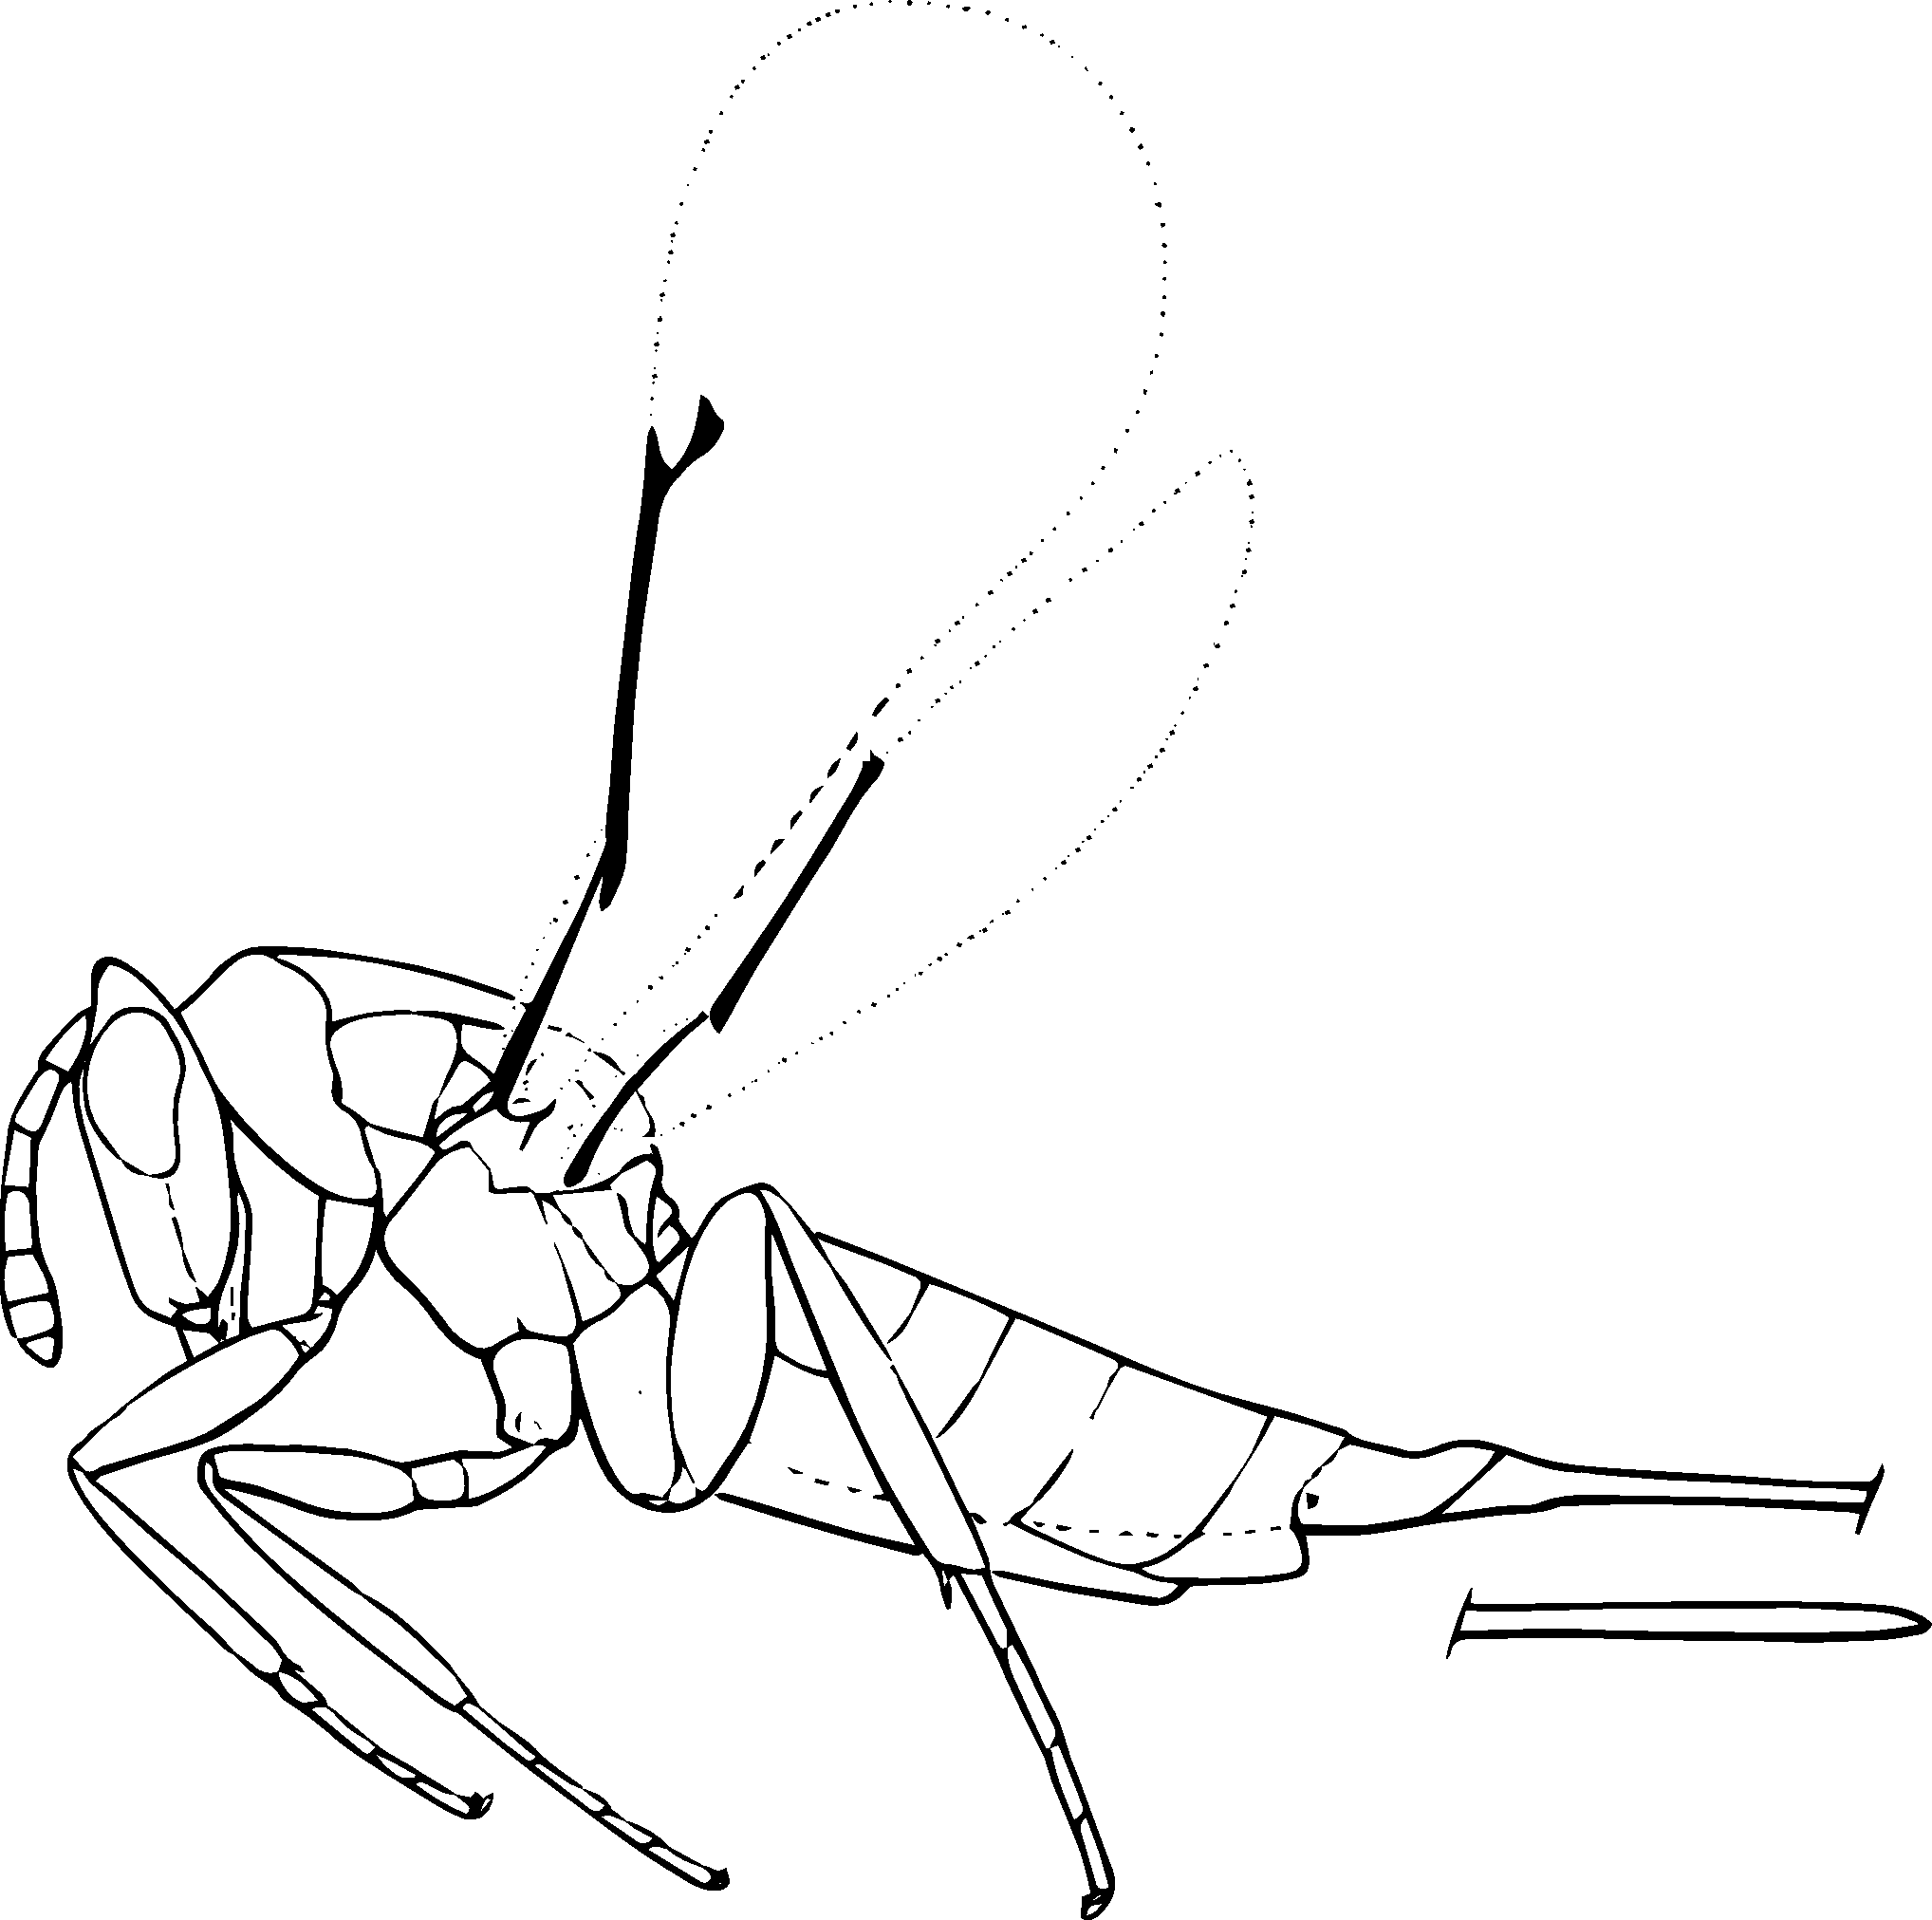
\includegraphics[width=\textwidth]{hymenoptera/EulophidHabitus}}
  \caption{Eulophidae}
  \label{fig:eulophid}
\end{subfigure}
\caption{Chalcidoidea. \textbf{(a)} Chalcididae lateral habitus \citep[][Fig. 212]{goulet1993hymenoptera}; \textbf{(b)} Eulophidae habitus \citep[][Fig. 228]{goulet1993hymenoptera}}
\label{fig:xxxxxx}
\end{figure}

\subsubsection{Eulophidae}\index{Eulophidae}
\noindent{}\textit{Diagnostic characters:} Antennal funicle with 4 or fewer antennomeres; tarsi 4-segmented (figure \ref{fig:eulophid}); apical spur of front tibiae short and straight; small, often black, brown, or blue.\vspace{3mm}

\noindent{}\textit{Natural history:} More than 4,300 species have been described, and they are biologically quite  diverse. Most species develop as parasitoids of other insects, especially Holometabola, but some species are gall-makers.\vspace{3mm}

\subsubsection{Encyrtidae}\index{Encyrtidae}
\noindent{}\textit{Diagnostic characters:} mesopleuron strongly convex, without grooves (figure \ref{fig:encyrt1}); tarsi usually 5-segmented; if tarsi 4-segmented, funicle with 5+ antennomeres; apical spur of middle tibiae large; usually rather stout-bodied and very small; cerci distinctly anterior to apical abdominal margin (figure \ref{fig:encyrt2}).\vspace{3mm}

\noindent{}\textit{Natural history:} There are $\sim$3,700 described species worldwide. Like other chalcidoids, this lineage is biologically diverse. Most species are parasitoids of insect eggs or  of sternorrhynchans, and many are important biological control agents.\vspace{3mm}

\begin{figure}[ht!]
  \centering
\begin{subfigure}[ht!]{0.55\textwidth}
\reflectbox{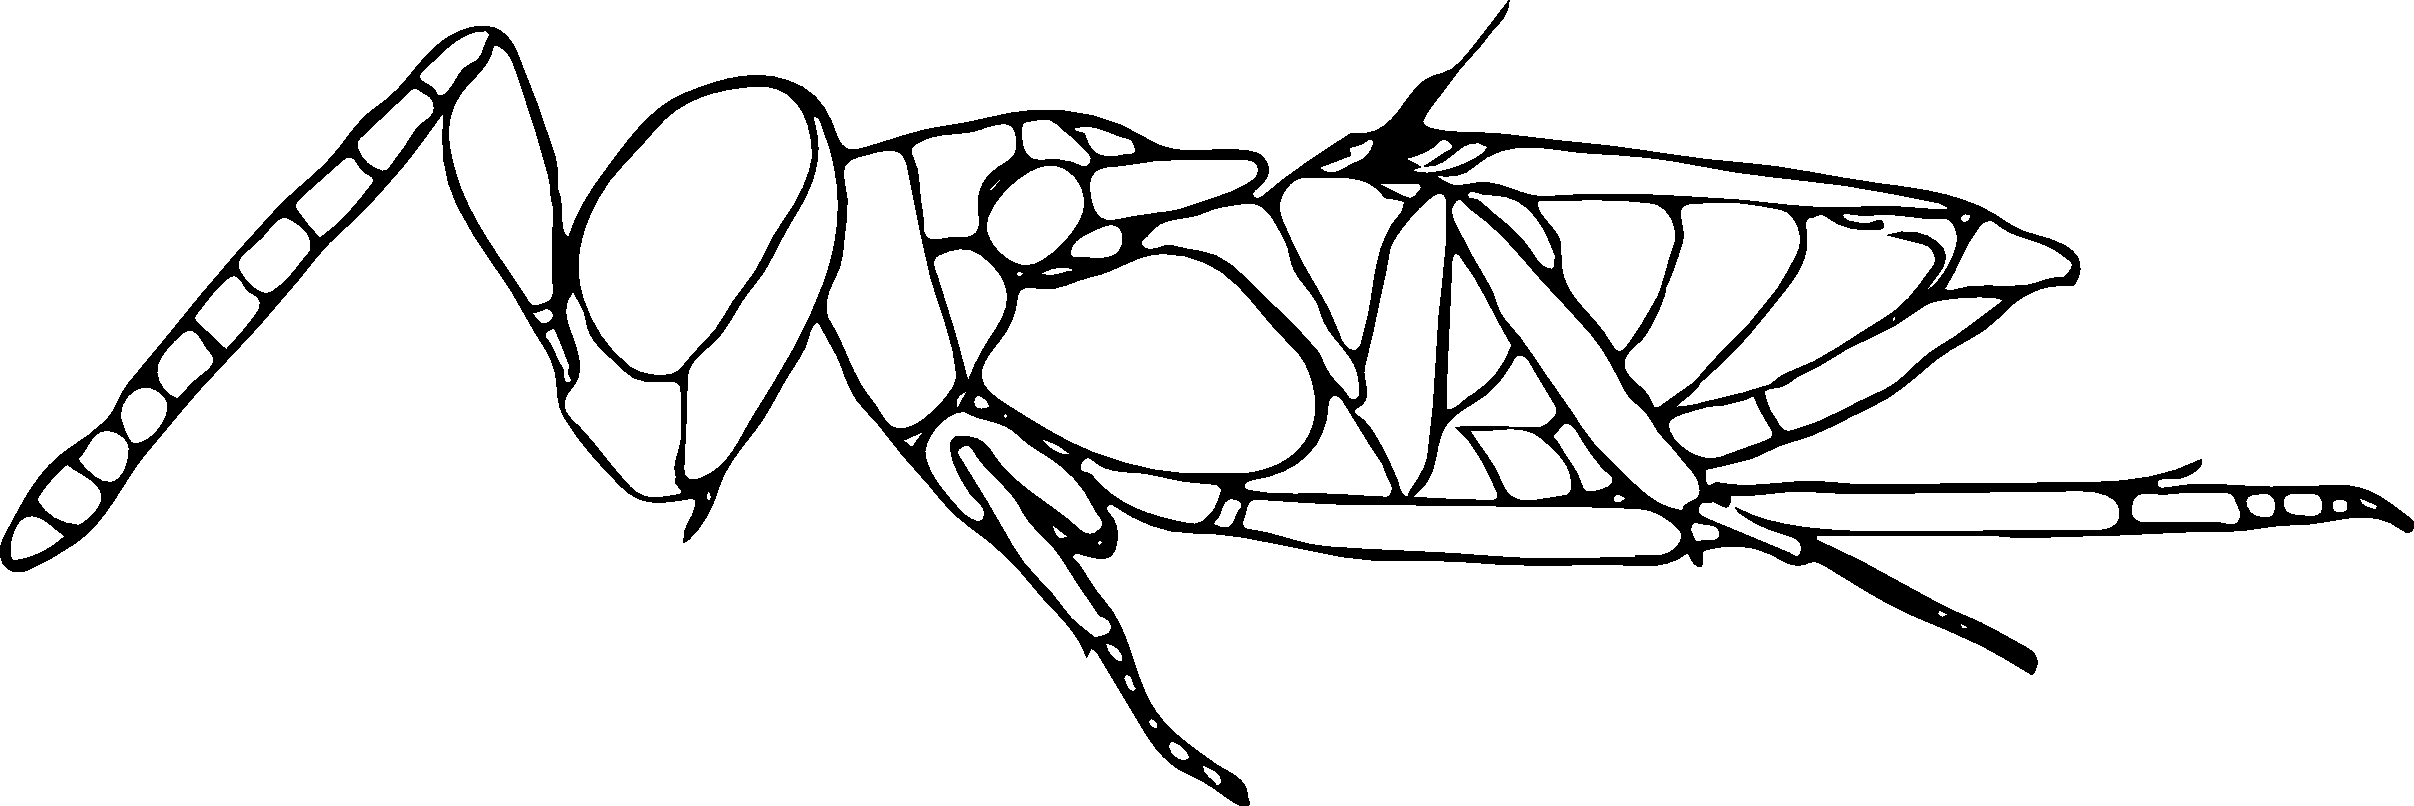
\includegraphics[width=\textwidth]{hymenoptera/EncyrtidHabitus}}
  \caption{}
  \label{fig:encyrt1}
\end{subfigure}
    \hfill
\begin{subfigure}[ht!]{0.35\textwidth}
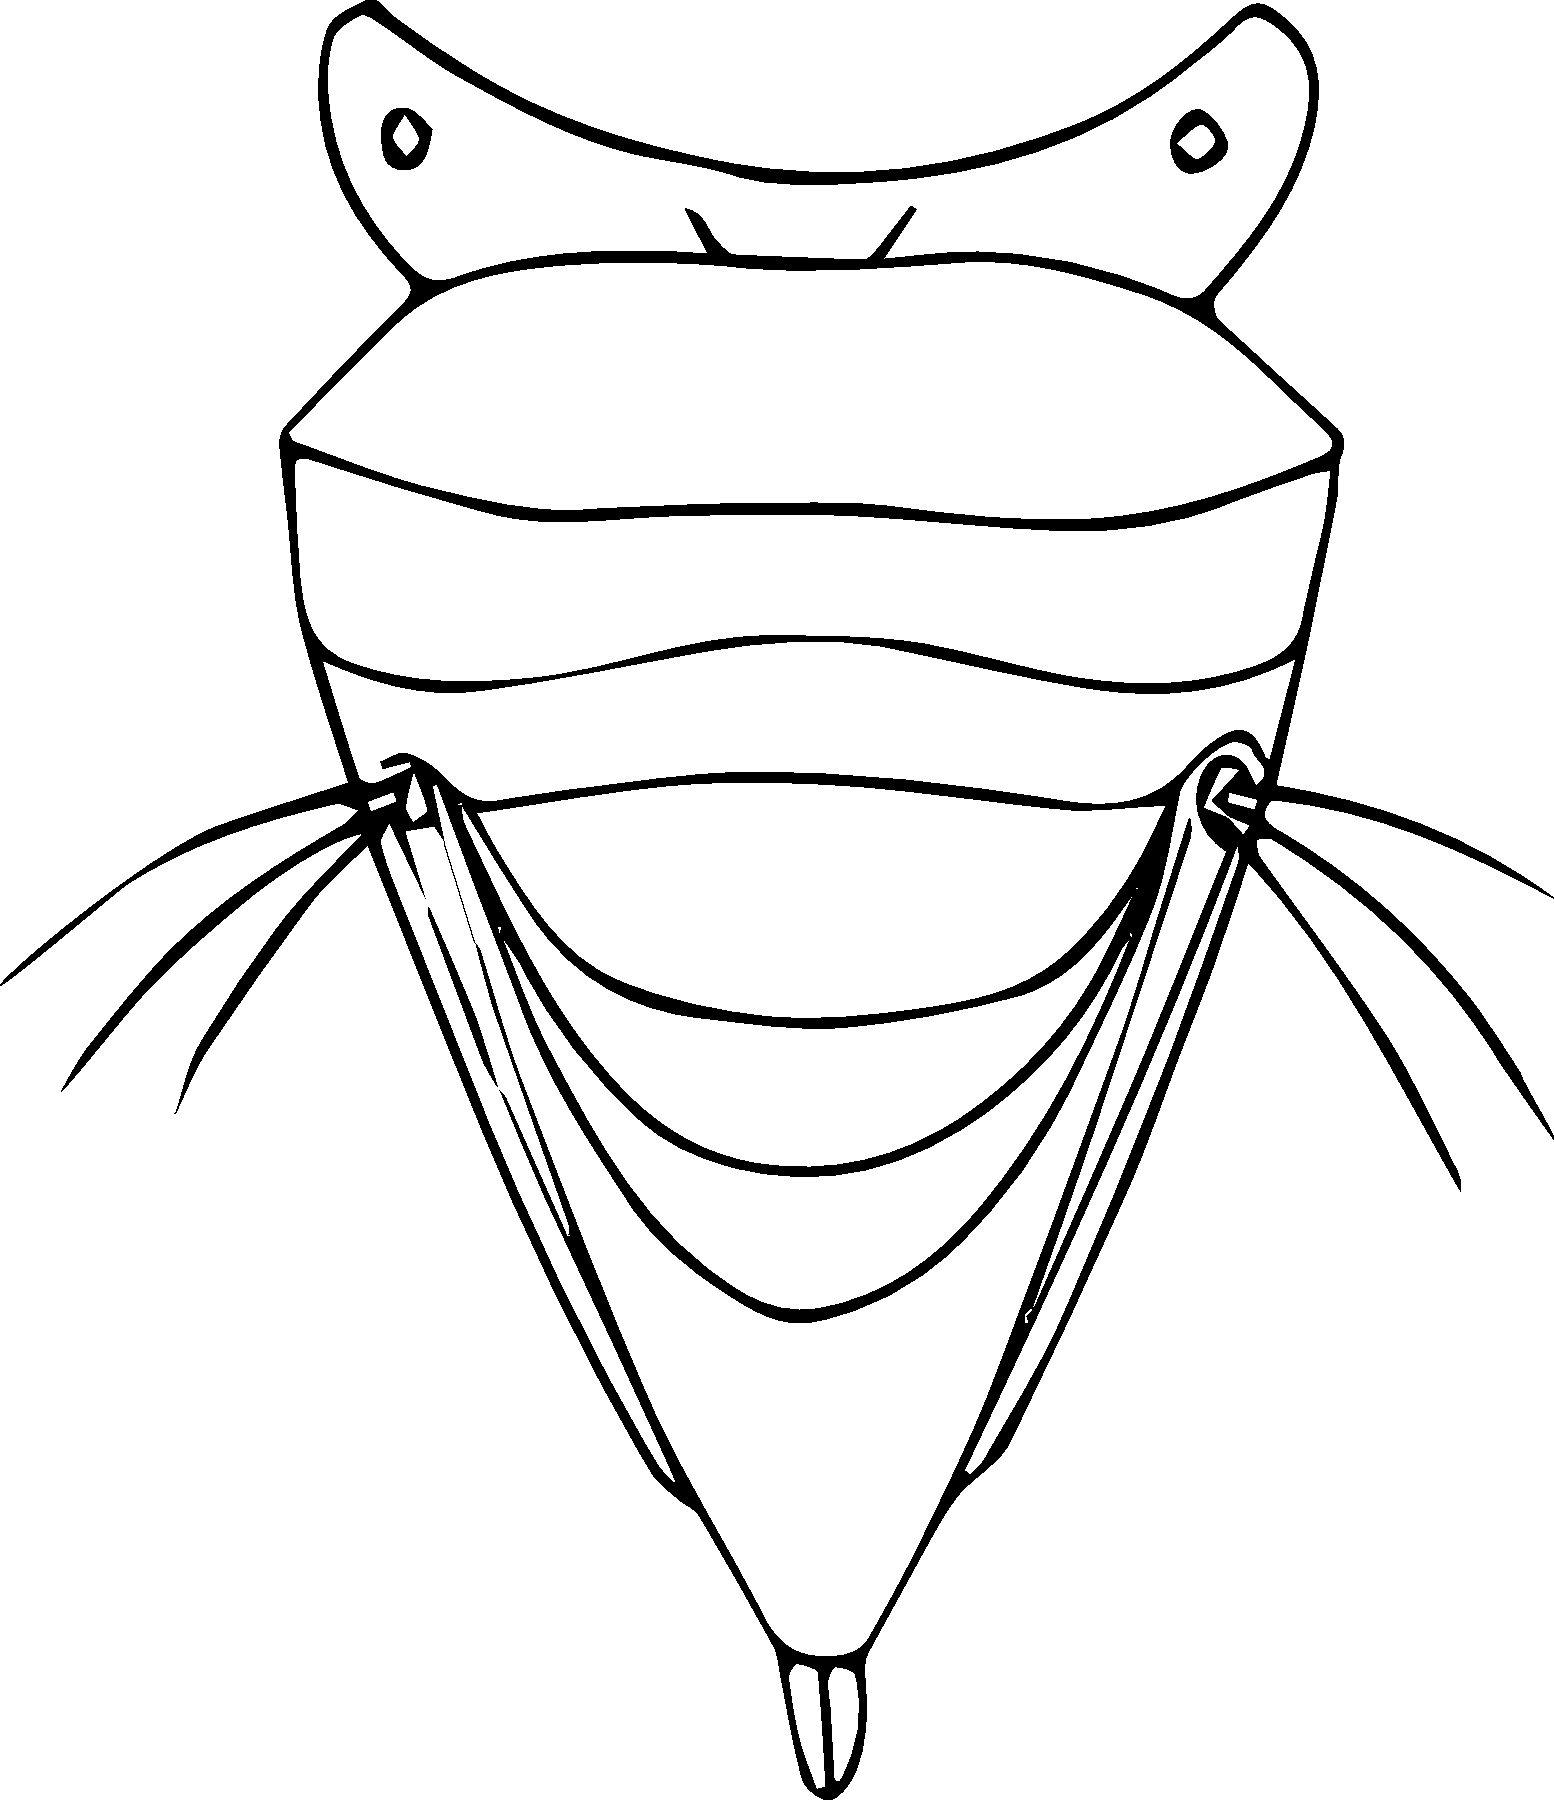
\includegraphics[angle=270,width=\textwidth]{hymenoptera/EncyrtidMetasoma}
  \caption{}
  \label{fig:encyrt2}
\end{subfigure}
    \caption{Encyrtidae. \textbf{(a)} Habitus \citep[redrawn from][]{nearcticChalcidoids}; \textbf{(b)} metasoma in dorsal view \citep[][pg. 581]{goulet1993hymenoptera}}\label{fig:encyrt}
\end{figure}

\subsubsection{Mymaridae (fairyflies)}\index{Mymaridae}
\noindent{}\textit{Diagnostic characters:} Body typically very small (these wasps are parasitoids of insect eggs); head with H-shaped complex bar-like structures on face (trabeculae); wings fringed; hind wing stalked proximally.\vspace{3mm}

\noindent{}\textit{Natural history:} There are \textgreater1,400 known species, all of which are (probably) parasitoids of insect eggs. This family includes the smallest known insect (\textit{Dicopomorpha echmepterygis} Mockford, 1997) and the smallest known flying insect (\textit{Kikiki huna} Huber \& Noyes 2013). The facial trabeculae likely correspond to an egg-bursting structure that facilitates eclosion and escape from the host remains.

\begin{figure}[ht!]
  \centering
\begin{subfigure}[ht!]{0.5\textwidth}
    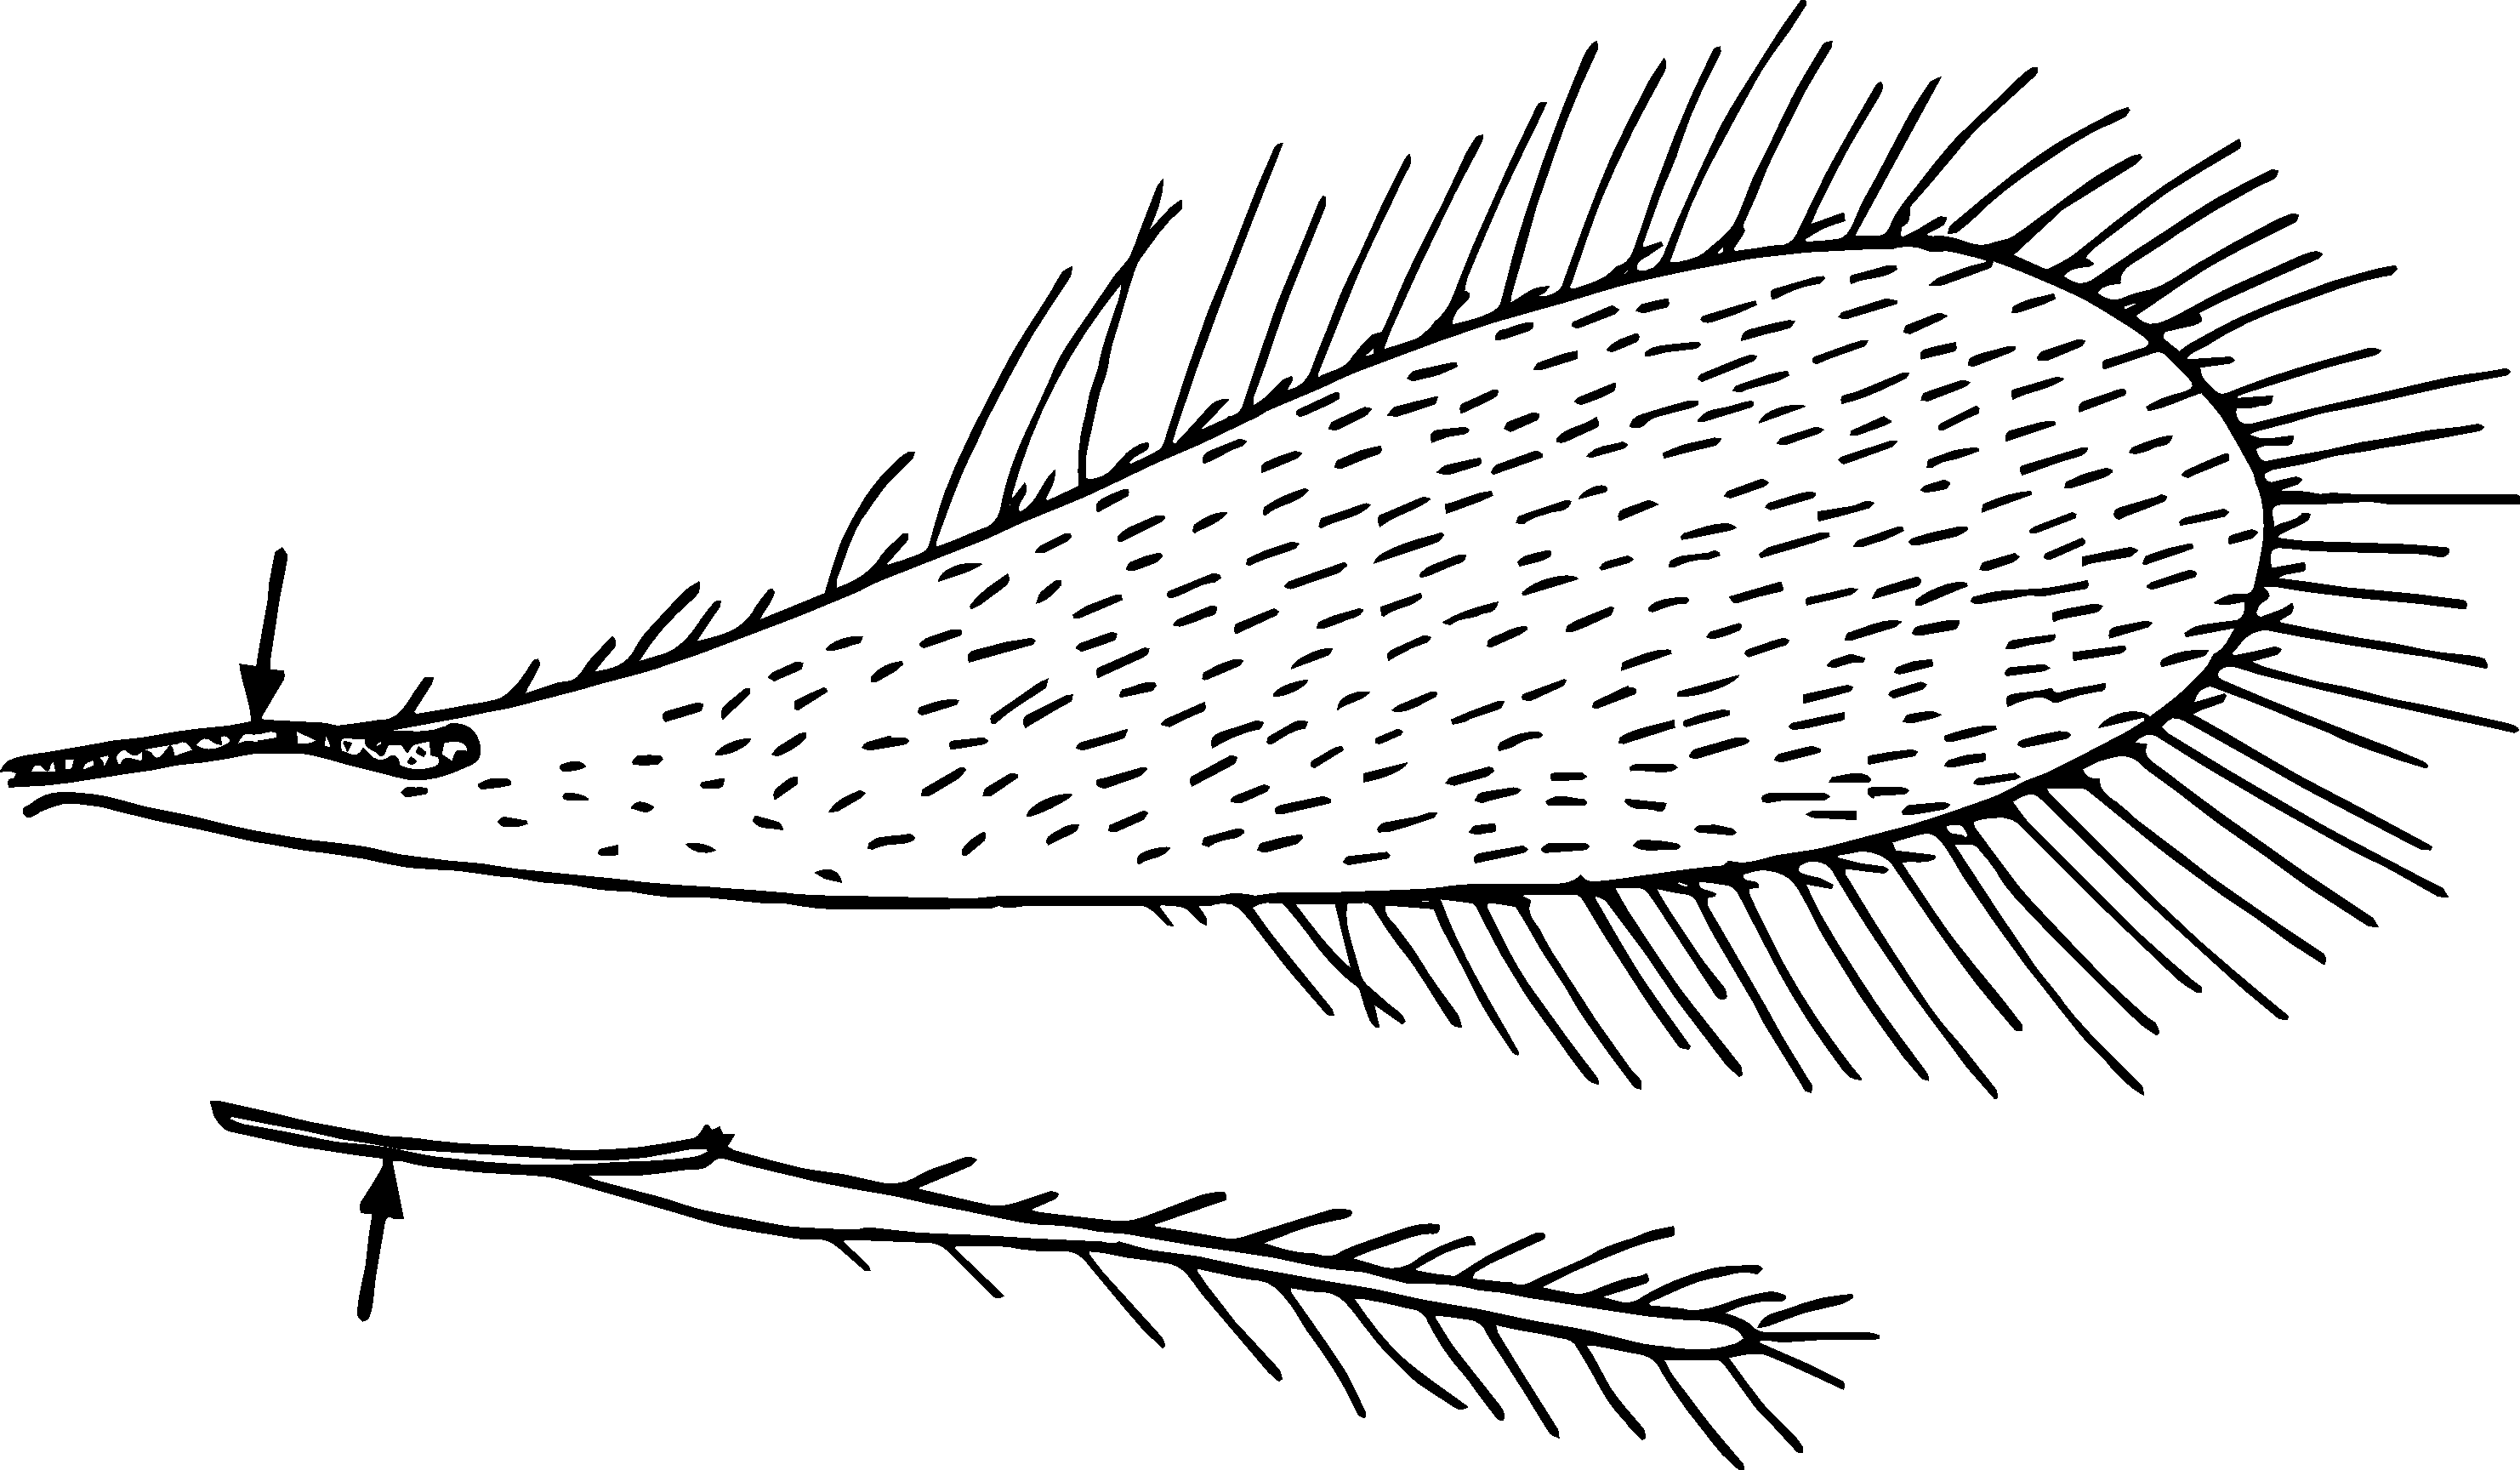
\includegraphics[width=\textwidth]{hymenoptera/MymaridWings}
  \caption{Wings}
  \label{fig:mymarid1}
\end{subfigure}
    \qquad
\begin{subfigure}[ht!]{0.28\textwidth}
    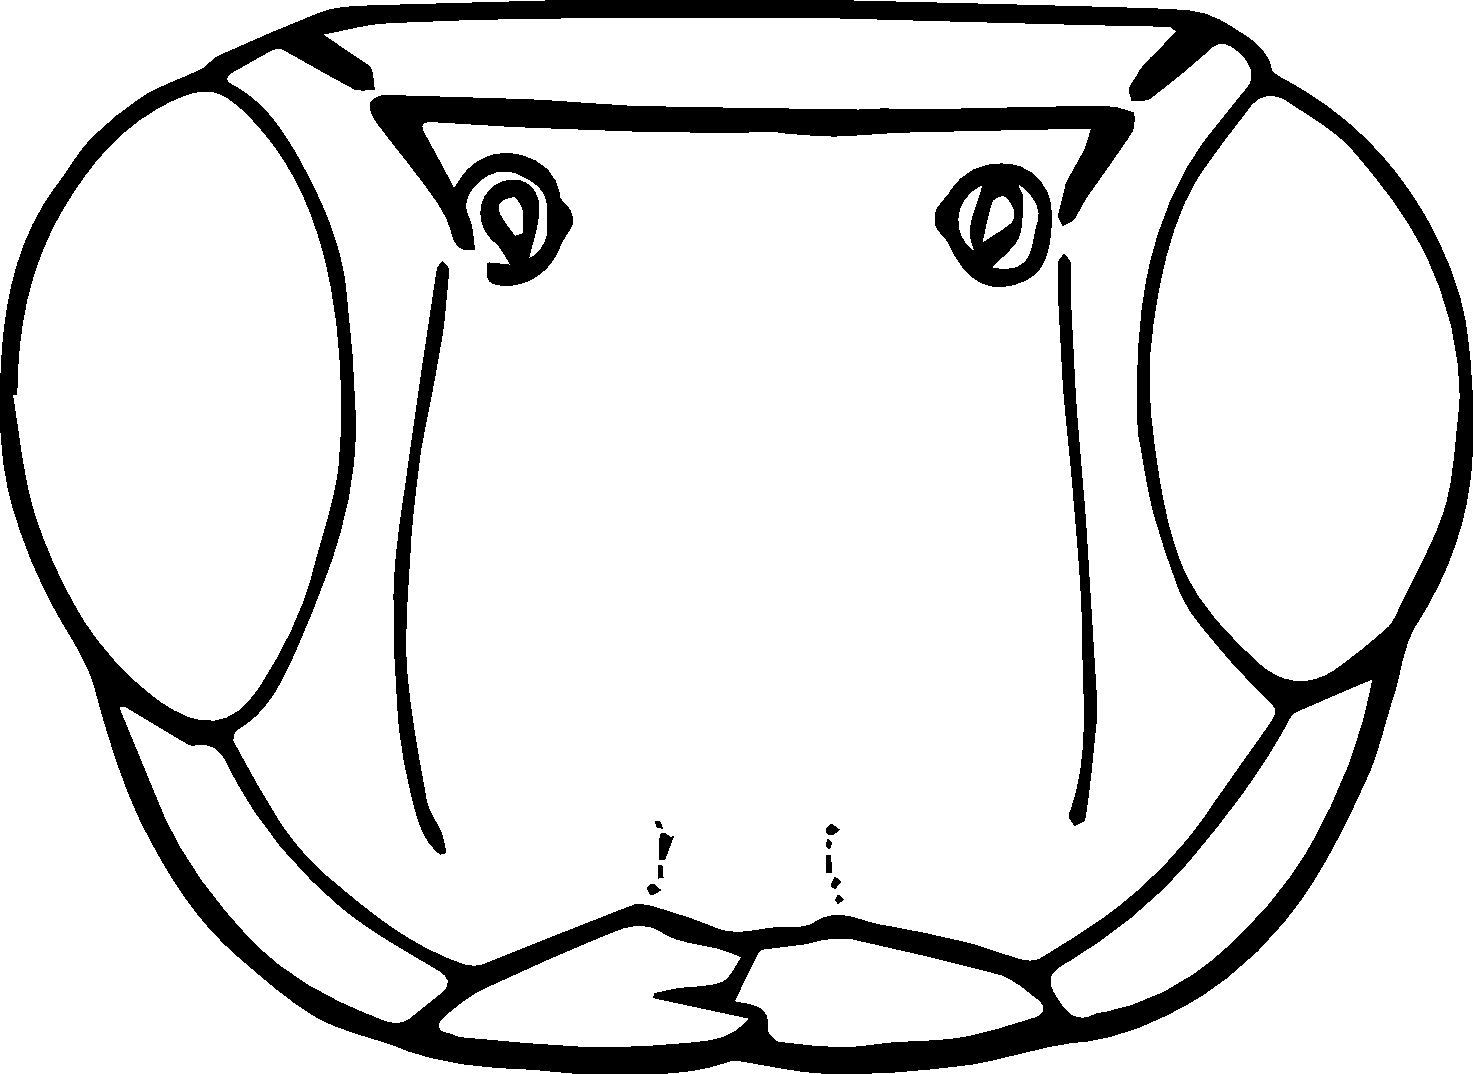
\includegraphics[width=\textwidth]{hymenoptera/MymaridHead}
  \caption{Head in anterior view}
  \label{fig:mymarid2}
\end{subfigure}
    \caption{Mymaridae \citep[][pg. 87]{goulet1993hymenoptera}}\label{fig:mymarids}
\end{figure}

\paragraph*{Aculeata}\index{Aculeata} In Aculeata, the egg does not enter the ovipositor assembly prior to deposition but rather leaves the metasoma anterior to the ovipositor. The ovipositor functions only to inject venom gland products (\textit{i.e.}, venom). Besides the structure of the ovipositor, the monophyly of Aculeata is supported mostly by indistinct internal characters (\textit{e.g.}, the shape, pattern and presence/absence of thoracic muscles). The only distinct synapomorphy of the infraorder is the presence of the supramesopleural sclerite (sms), that partially obscures the second thoracic spiracle. (Caveat: The sms is absent from a few Aculeata and \textit{present} in some non-aculeates, like Evaniidae and Trigonalidae.)\vspace{3mm}

\noindent{}Besides the above-mentioned synapomorphies, Aculeata can be superficially characterized by their well-developed wing venation (but see some ``Chrysidoidea'', \textit{e.g.}, figure \ref{fig:bethylid1}), distinct wasp waist (unlike sawflies), well sclerotized metasomal sternites (unlike most Ichneumonoidea), having fewer than 11 flagellomeres (numerous Ichneumonoidea have more than 11 flagellomeres), and convex, almost bulbous metasoma.\vspace{3mm}

\noindent{}Traditionally the infraorder is subdivided into three superfamilies: Chrysidoidea, Apoidea, and Vespoidea. Only the monophyly of Apoidea is supported in the latest phylogenetic analyses.

\subsubsection{Bethylidae}\index{Bethylidae}
\noindent{}\textit{Diagnostic characters:} Body usually weakly sculptured and brown or black (not typically metallic); head usually prognathous (figure \ref{fig:bethylid1}); antenna with 11 (rarely 10 or 8) flagellomeres; pronotum with anterior flange, propleuron thus concealed in dorsal view; distal venation of wing reduced; metasoma with 6 or 7 exposed terga.\vspace{3mm}

\noindent{}\textit{Natural history:} This taxon includes \textgreater2,200 species, many of which are known to develop as parasitoids of holometabolous insects in concealed environments (\textit{e.g.}, wood-boring Coleoptera).

\begin{figure}[ht!]
  \centering
\begin{subfigure}[ht!]{0.28\textwidth}
    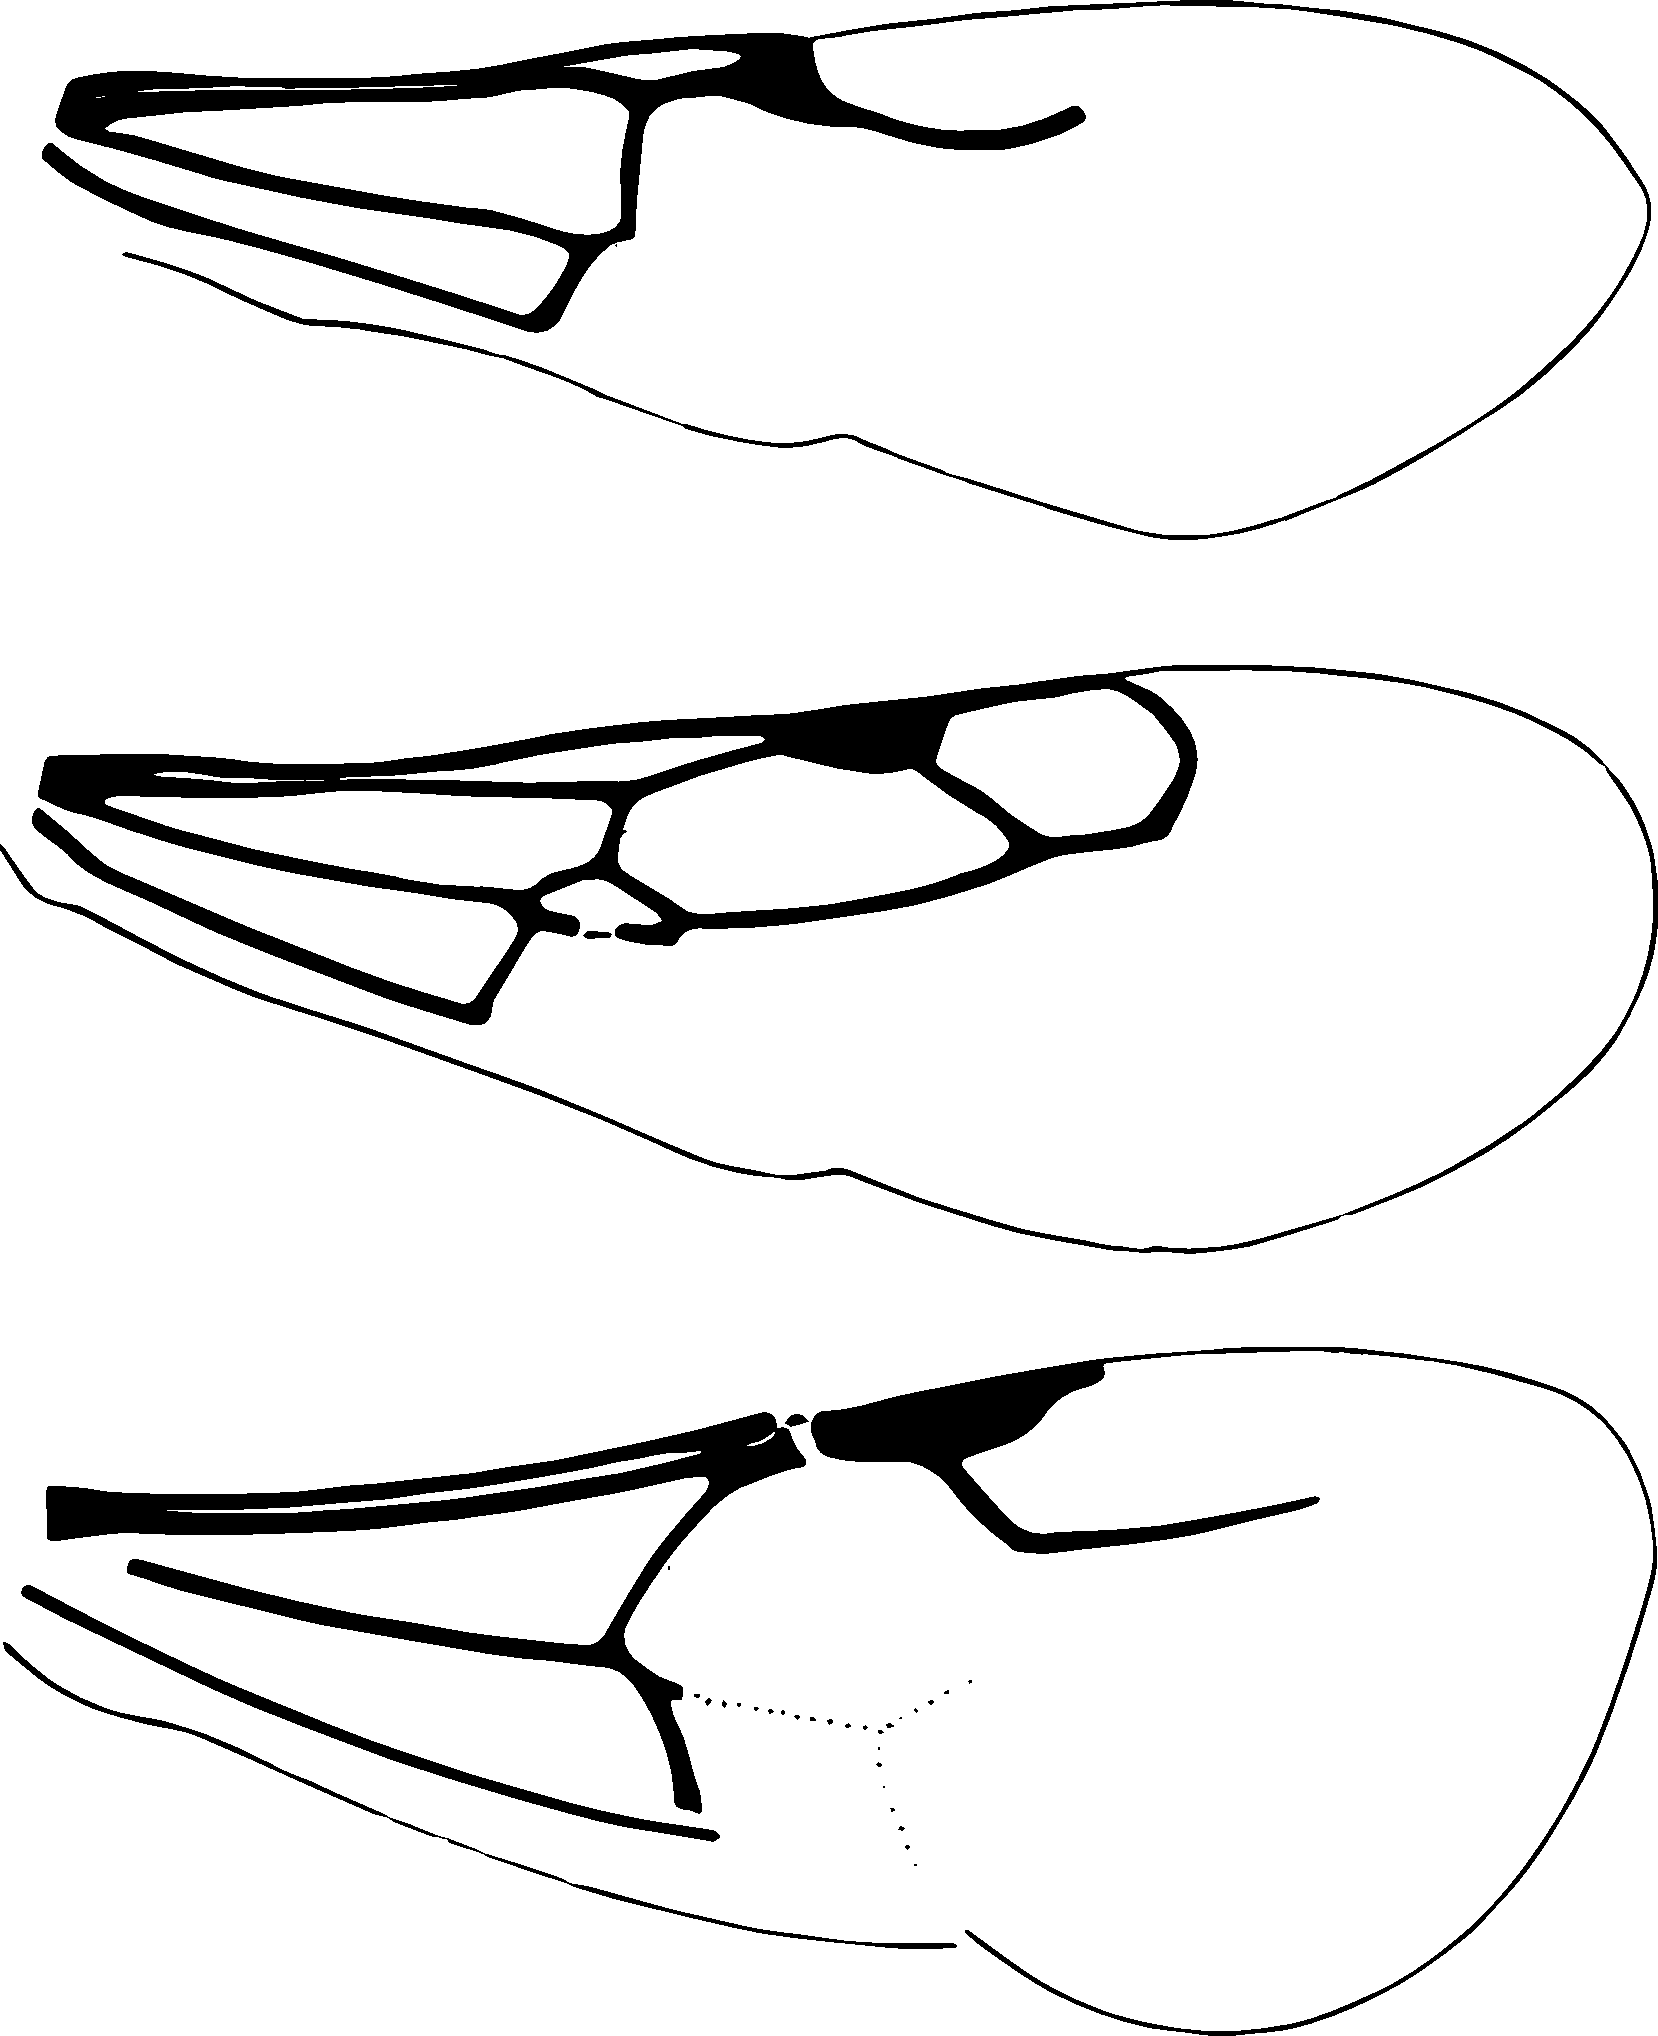
\includegraphics[width=\textwidth]{hymenoptera/BethylidWings}
  \caption{}
  \label{fig:bethylid1}
\end{subfigure}
    \qquad
\begin{subfigure}[ht!]{0.35\textwidth}
    \reflectbox{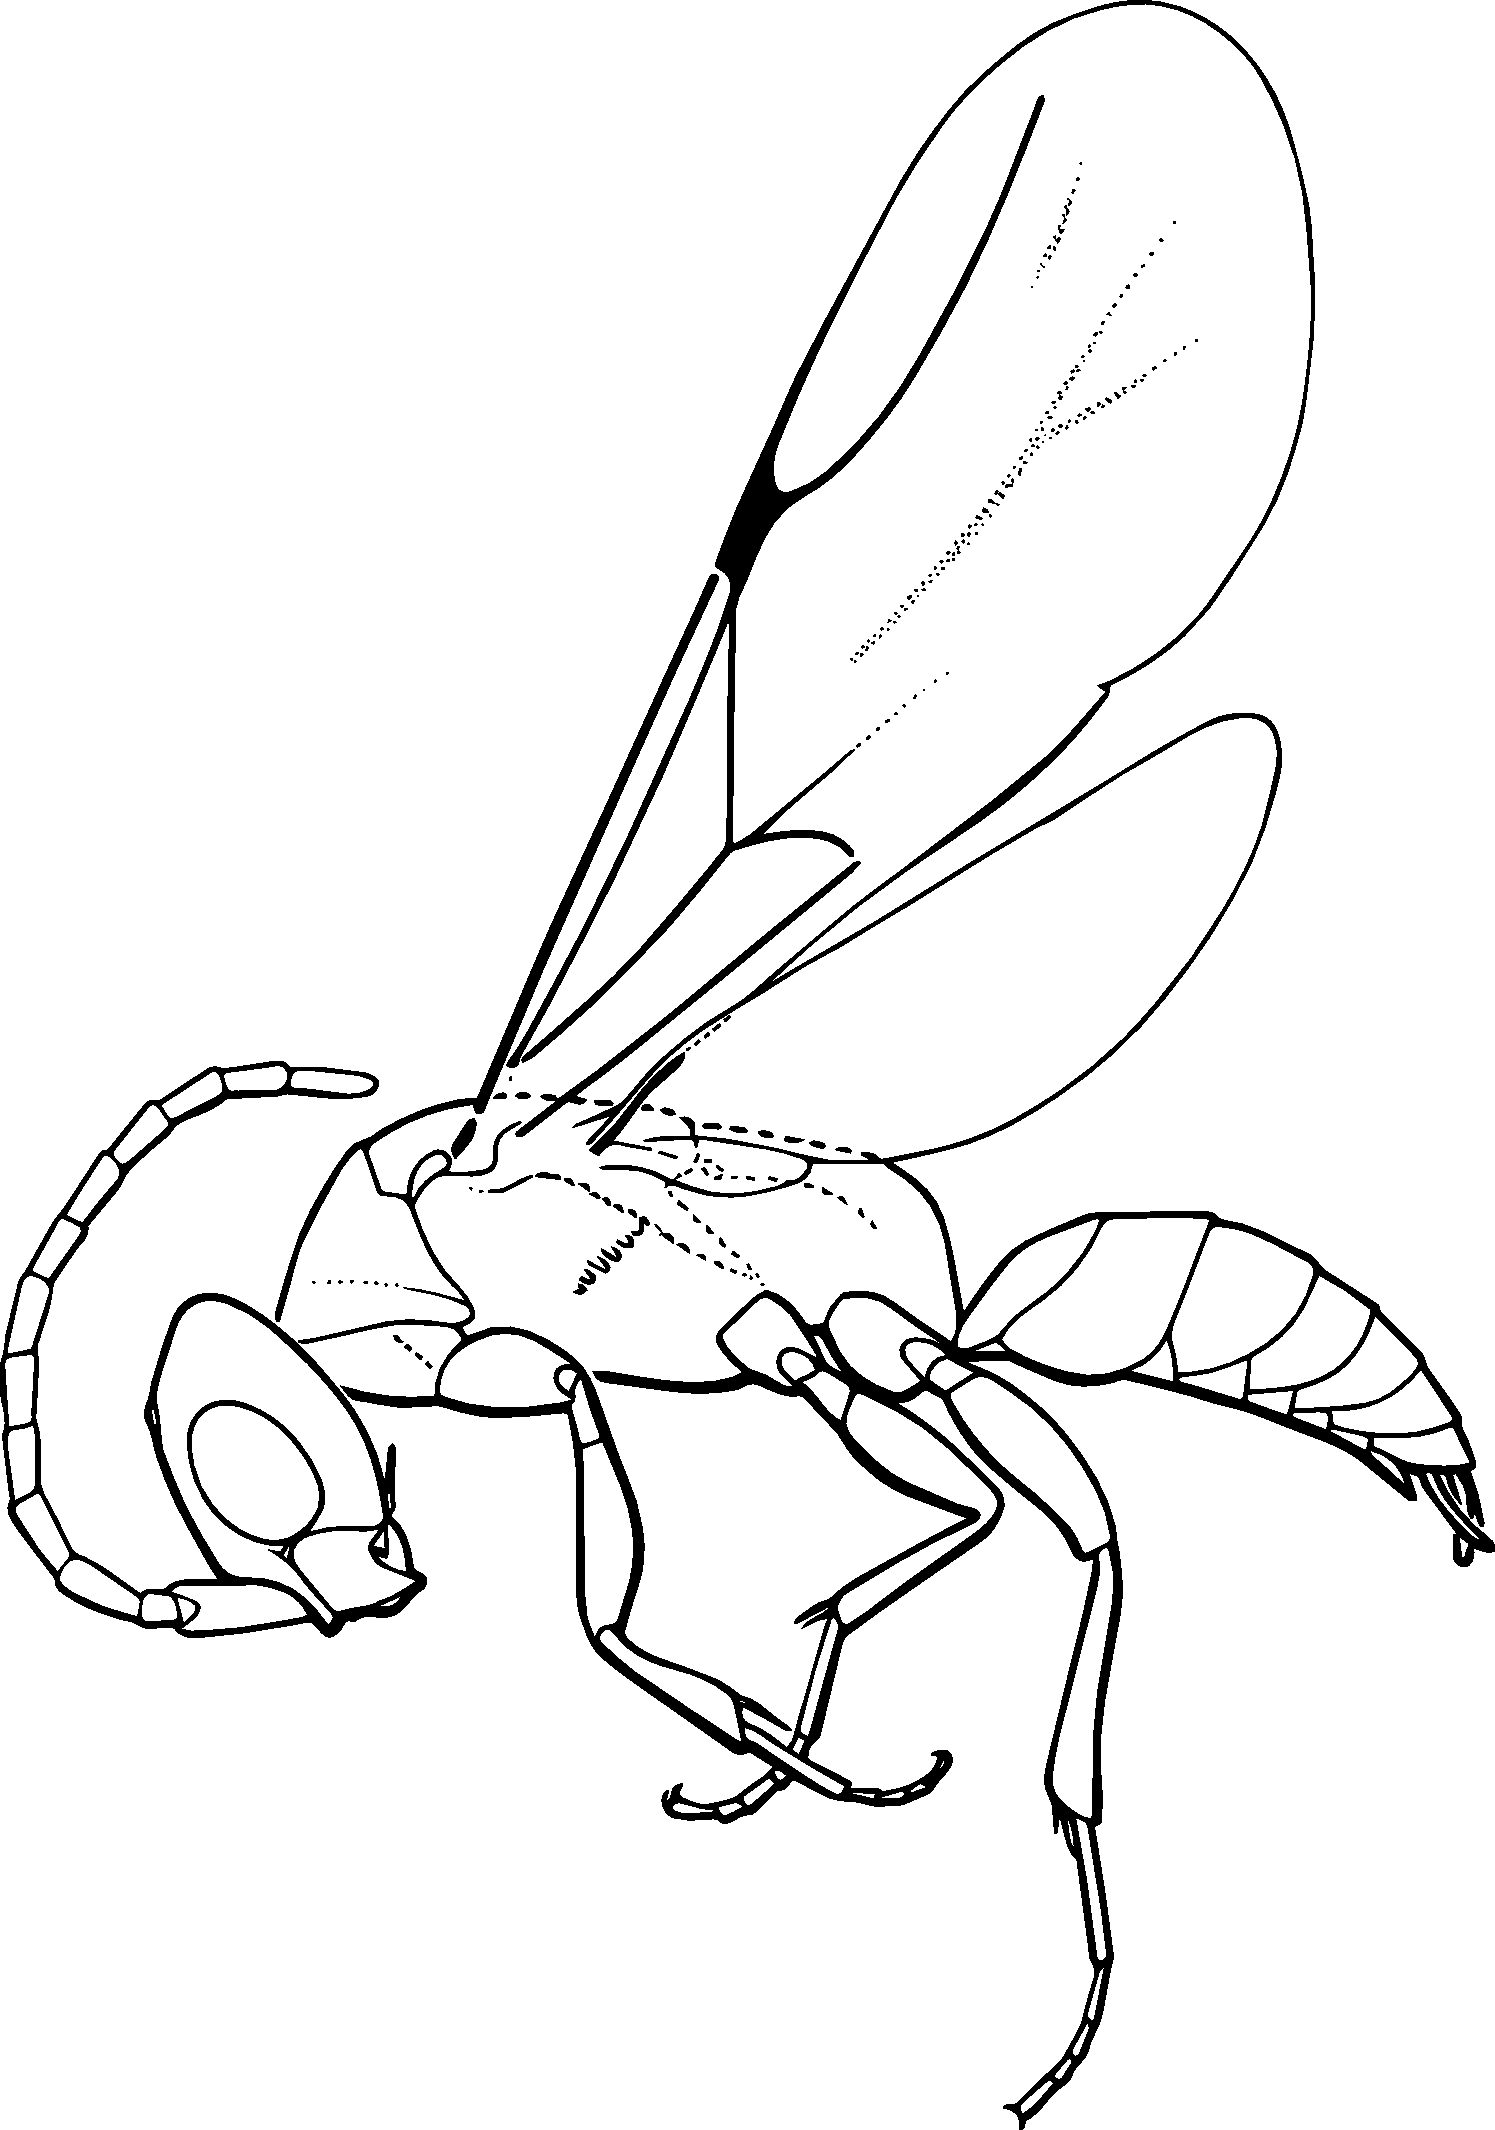
\includegraphics[width=\textwidth]{hymenoptera/BethylidHabitus}}
  \caption{}
  \label{fig:bethylid2}
\end{subfigure}
    \caption{Bethylidae. \textbf{(a)} Fore wings \citep[][pg. 134]{goulet1993hymenoptera}; \textbf{(b)} habitus \citep[][Fig. 37]{goulet1993hymenoptera}}\label{fig:bethylids}
\end{figure}

\subsubsection{Chrysididae (cuckoo wasps)}\index{Chrysididae}
\noindent{}\textit{Diagnostic characters:} Head typically hypognathous; antenna with 11 flagellomeres; pronotum with anterior flange, such that propleuron is concealed in dorsal view; pronotum with posterolateral apex usually well separated from tegula; metasoma usually with 5 or fewer exposed terga and strongly concave ventrally (figure \ref{fig:chrysididae}); usually strongly sculptured and metallic.\vspace{3mm}

\noindent{}\textit{Natural history:} Of the \textgreater3,000 known species, the majority likely develop as cleptoparasites of other aculeates. That is, most chrysidids lay their eggs in the nests of bees and wasps, and the subsequent larvae develop on the provisions and eggs located therein. Other species develop as parasitoids, for example in phasmatodean eggs.

\begin{figure}[ht!]
  \centering
    \reflectbox{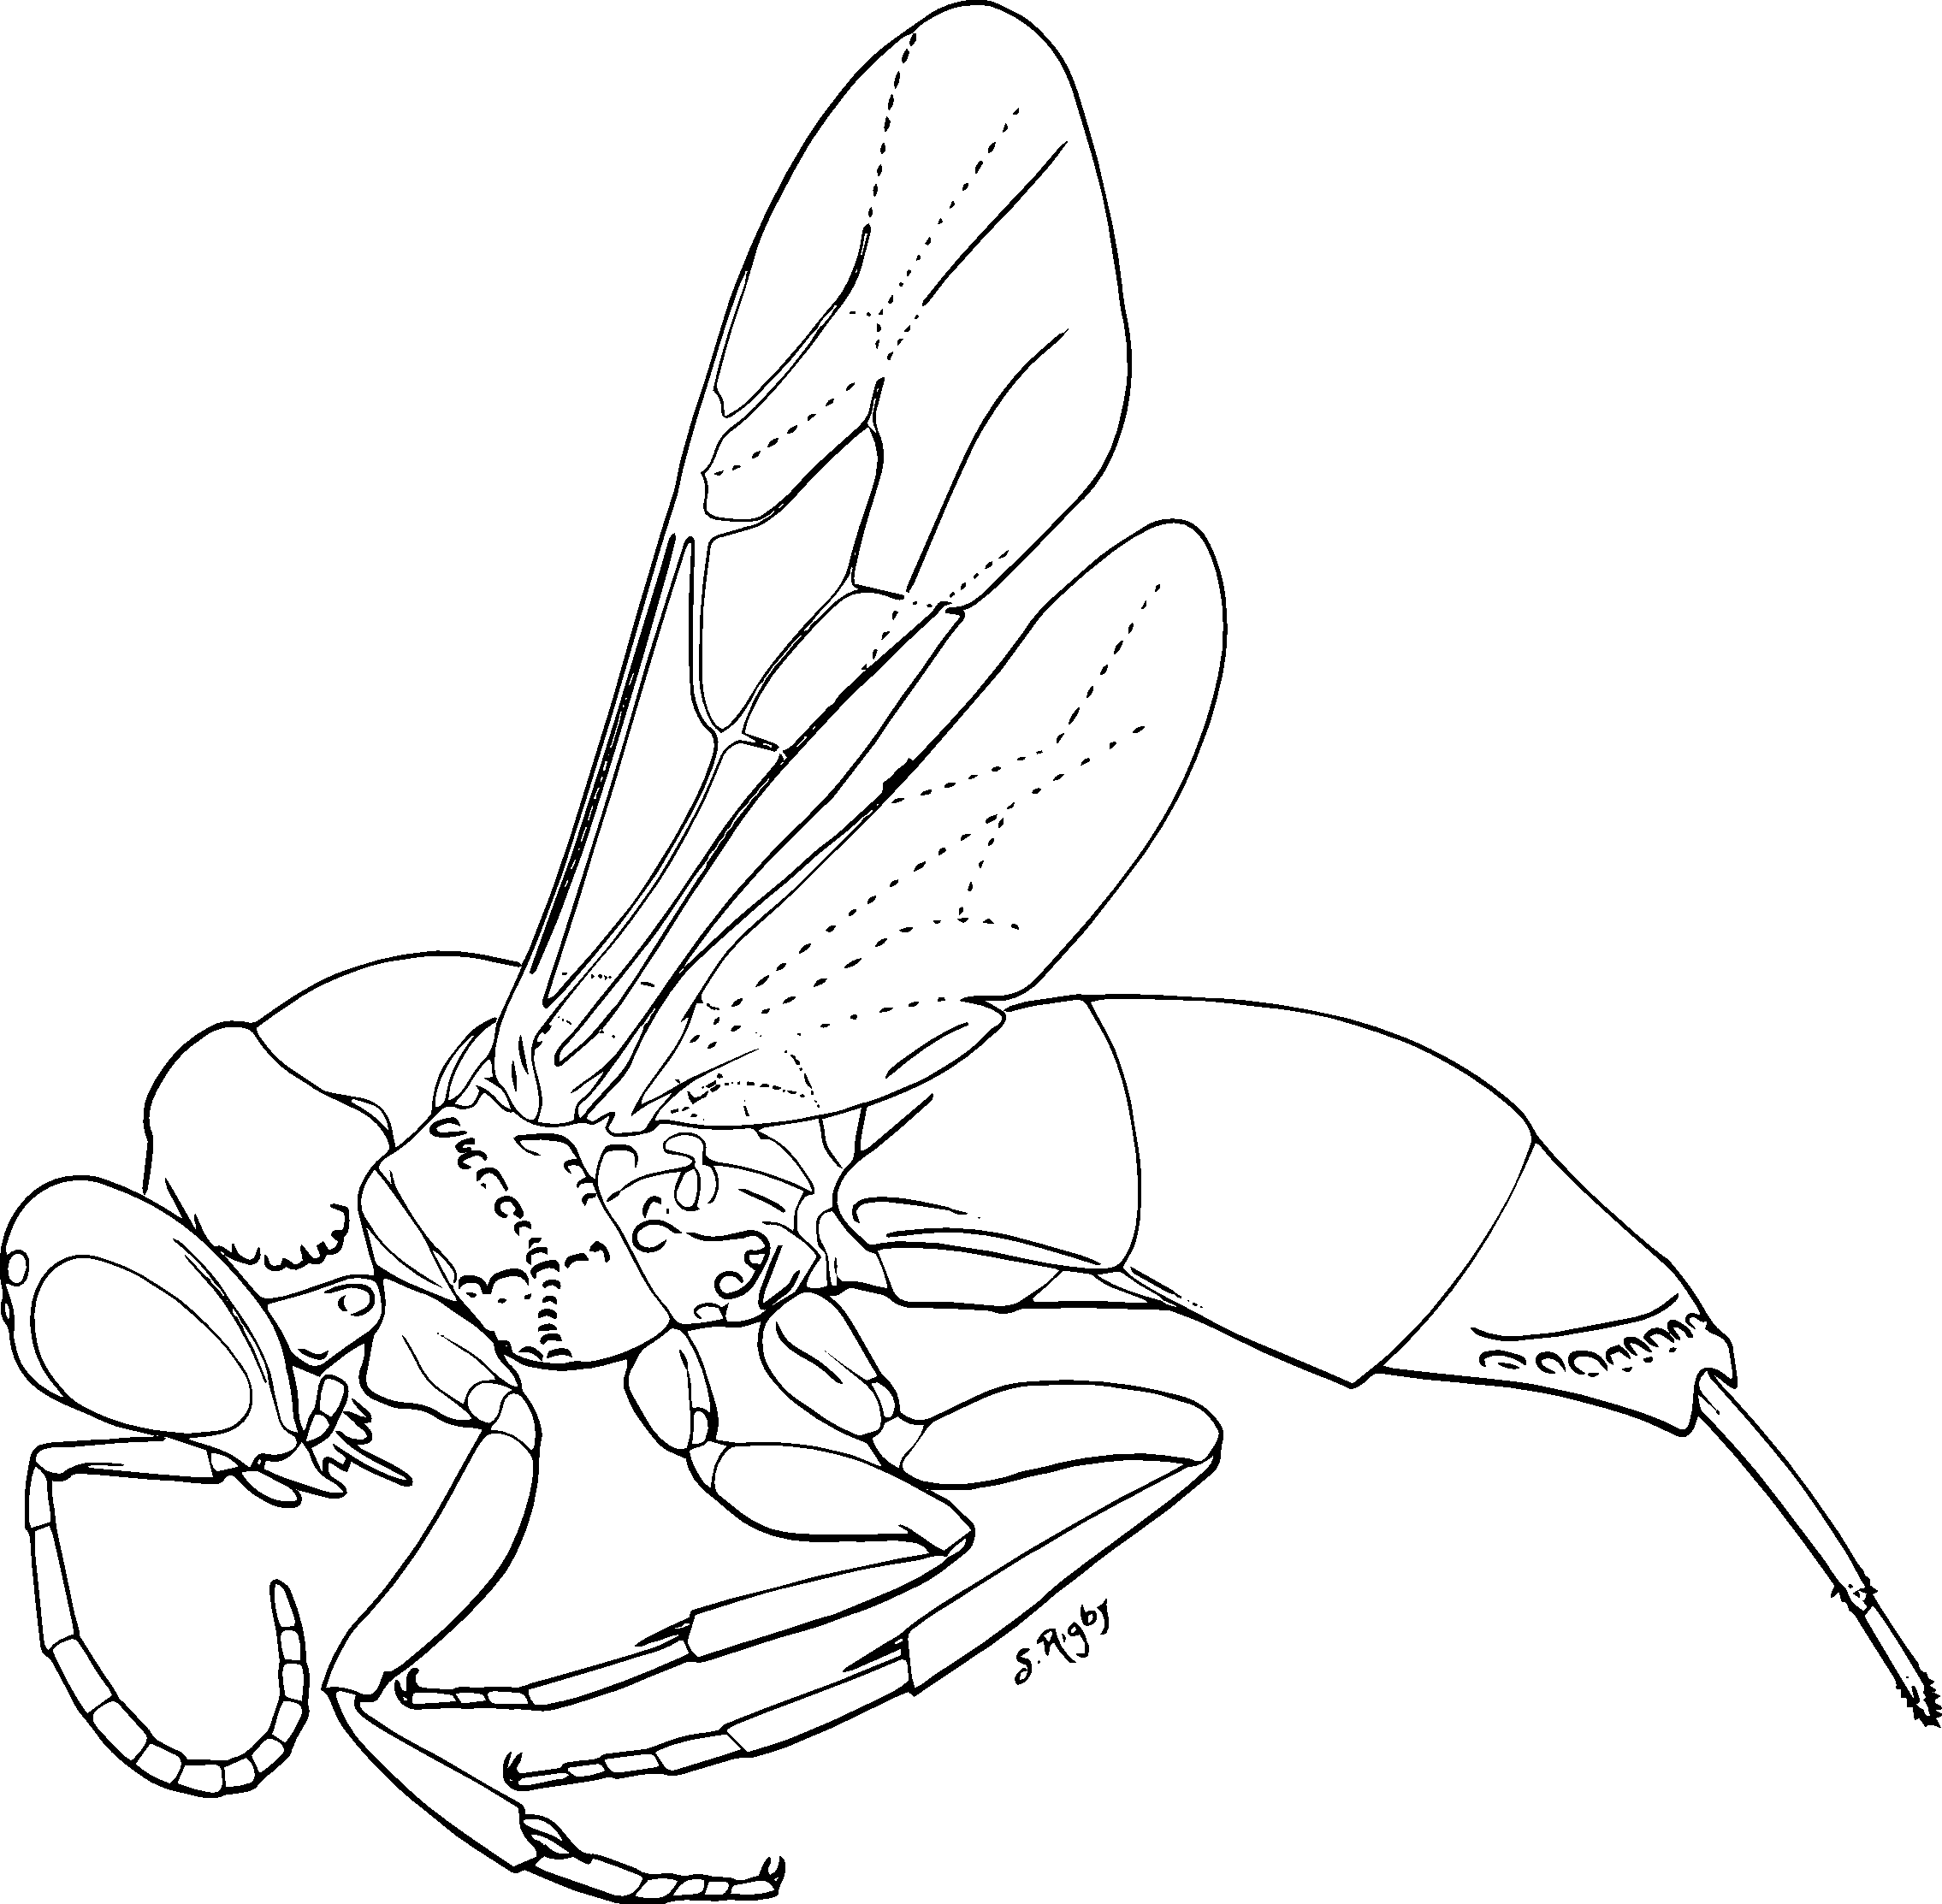
\includegraphics[width=0.45\textwidth]{hymenoptera/ChrysididHabitus}}
  \caption{Chrysididae lateral habitus \citep[][Fig. 42]{goulet1993hymenoptera}}
  \label{fig:chrysididae}
\end{figure}

\subsubsection{Tiphiidae}\index{Tiphiidae}
\noindent{}\textit{Diagnostic characters:} eye not usually ``notched''; mesosternum with laminate expansions on each side of midline covering bases of contiguous mesocoxae (figure \ref{fig:tiphiid1}), the expansions rarely reduced to small teeth; hind wing with deeply separated (jugal) lobe (figure \ref{fig:tiphiid2}); female usually with mesotibia and metatibia stout and spiny; metasomal segment 1 without a true node (like we see in Formicidae), although sometimes approaching it; male metasomal sternum 8 (hypopygium) usually forming a single upcurved hook (figure \ref{fig:tiphiid2}), the hypopygium sometimes simple or with 2--5 spines, and usually entirely exposed.\vspace{3mm}

\noindent{}\textit{Natural history:} More than 1,500 species of tiphiids have been described worldwide, and rearing records indicate that a majority are parasitoids of Coleoptera, especially Scarabaeidae.

\begin{figure}[ht!]
    \centering
    \begin{subfigure}[ht!]{0.4\textwidth}
        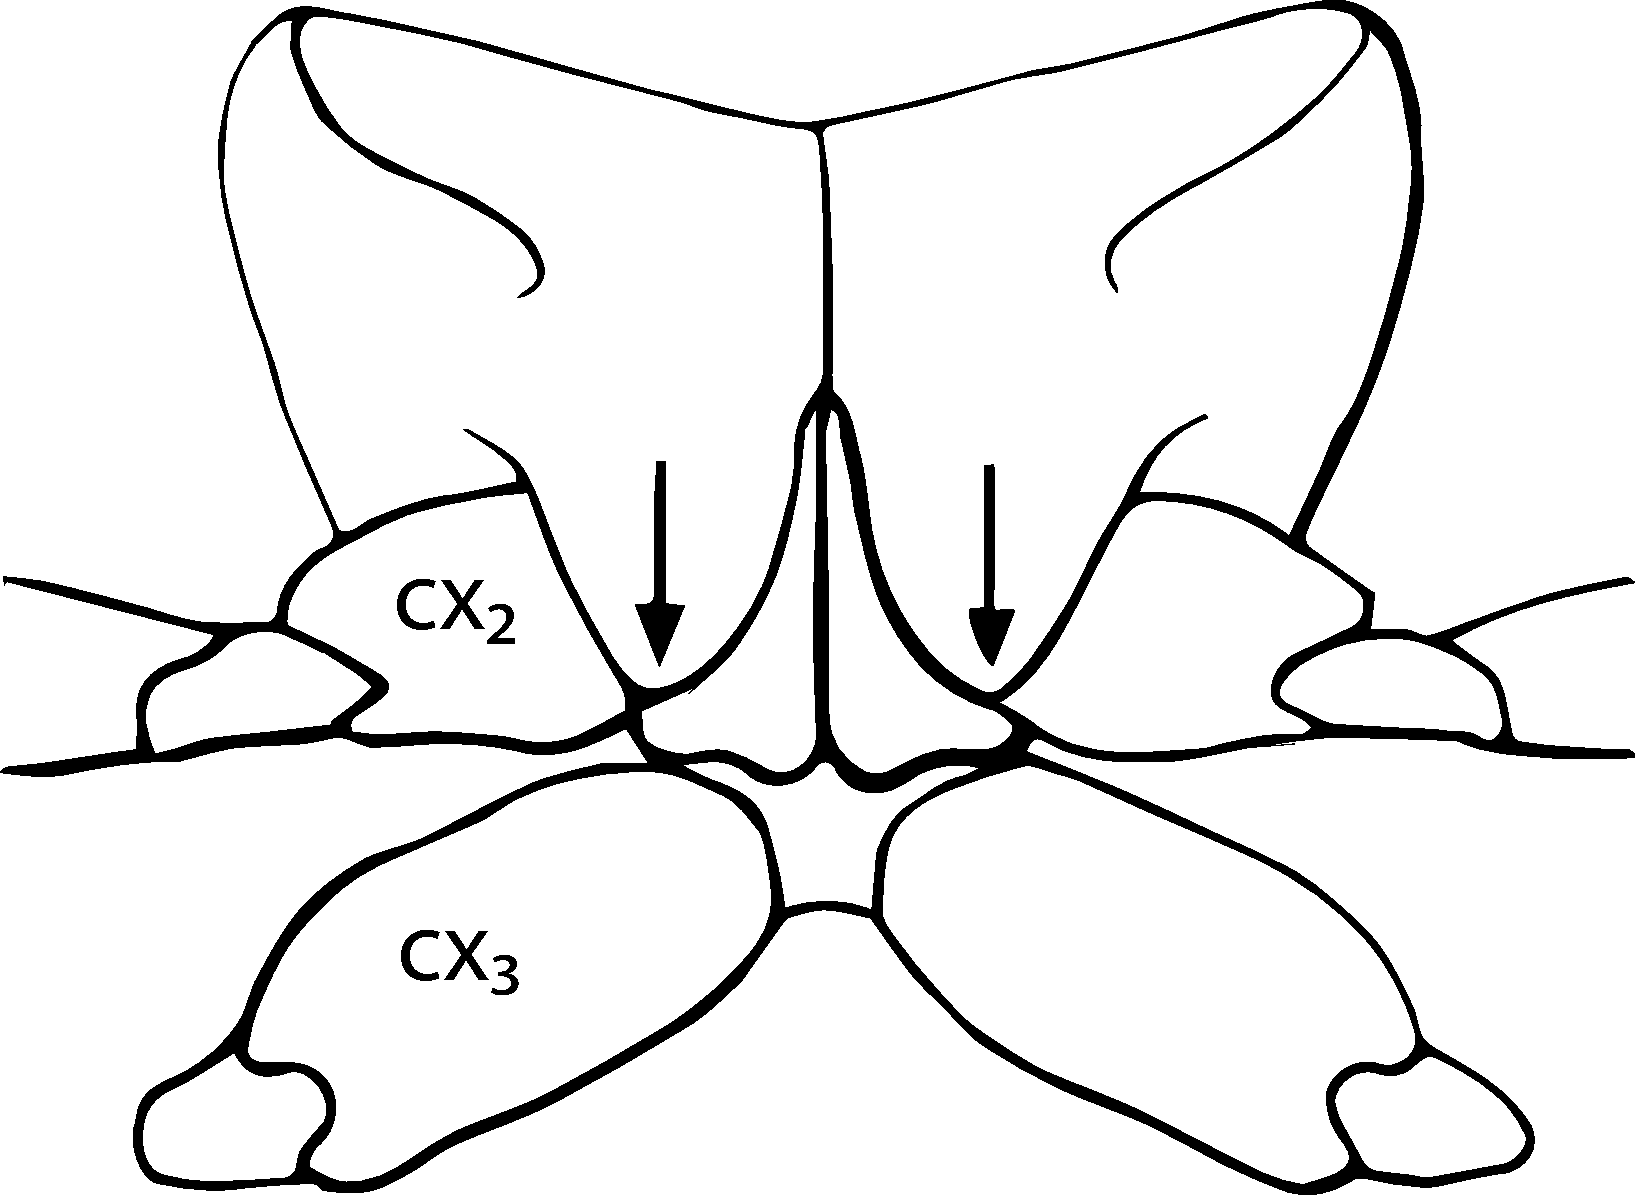
\includegraphics[width=\textwidth]{hymenoptera/TiphiidMesosoma}
        \caption{}
        \label{fig:tiphiid1}
    \end{subfigure}
    \qquad
    \begin{subfigure}[ht!]{0.45\textwidth}
        \reflectbox{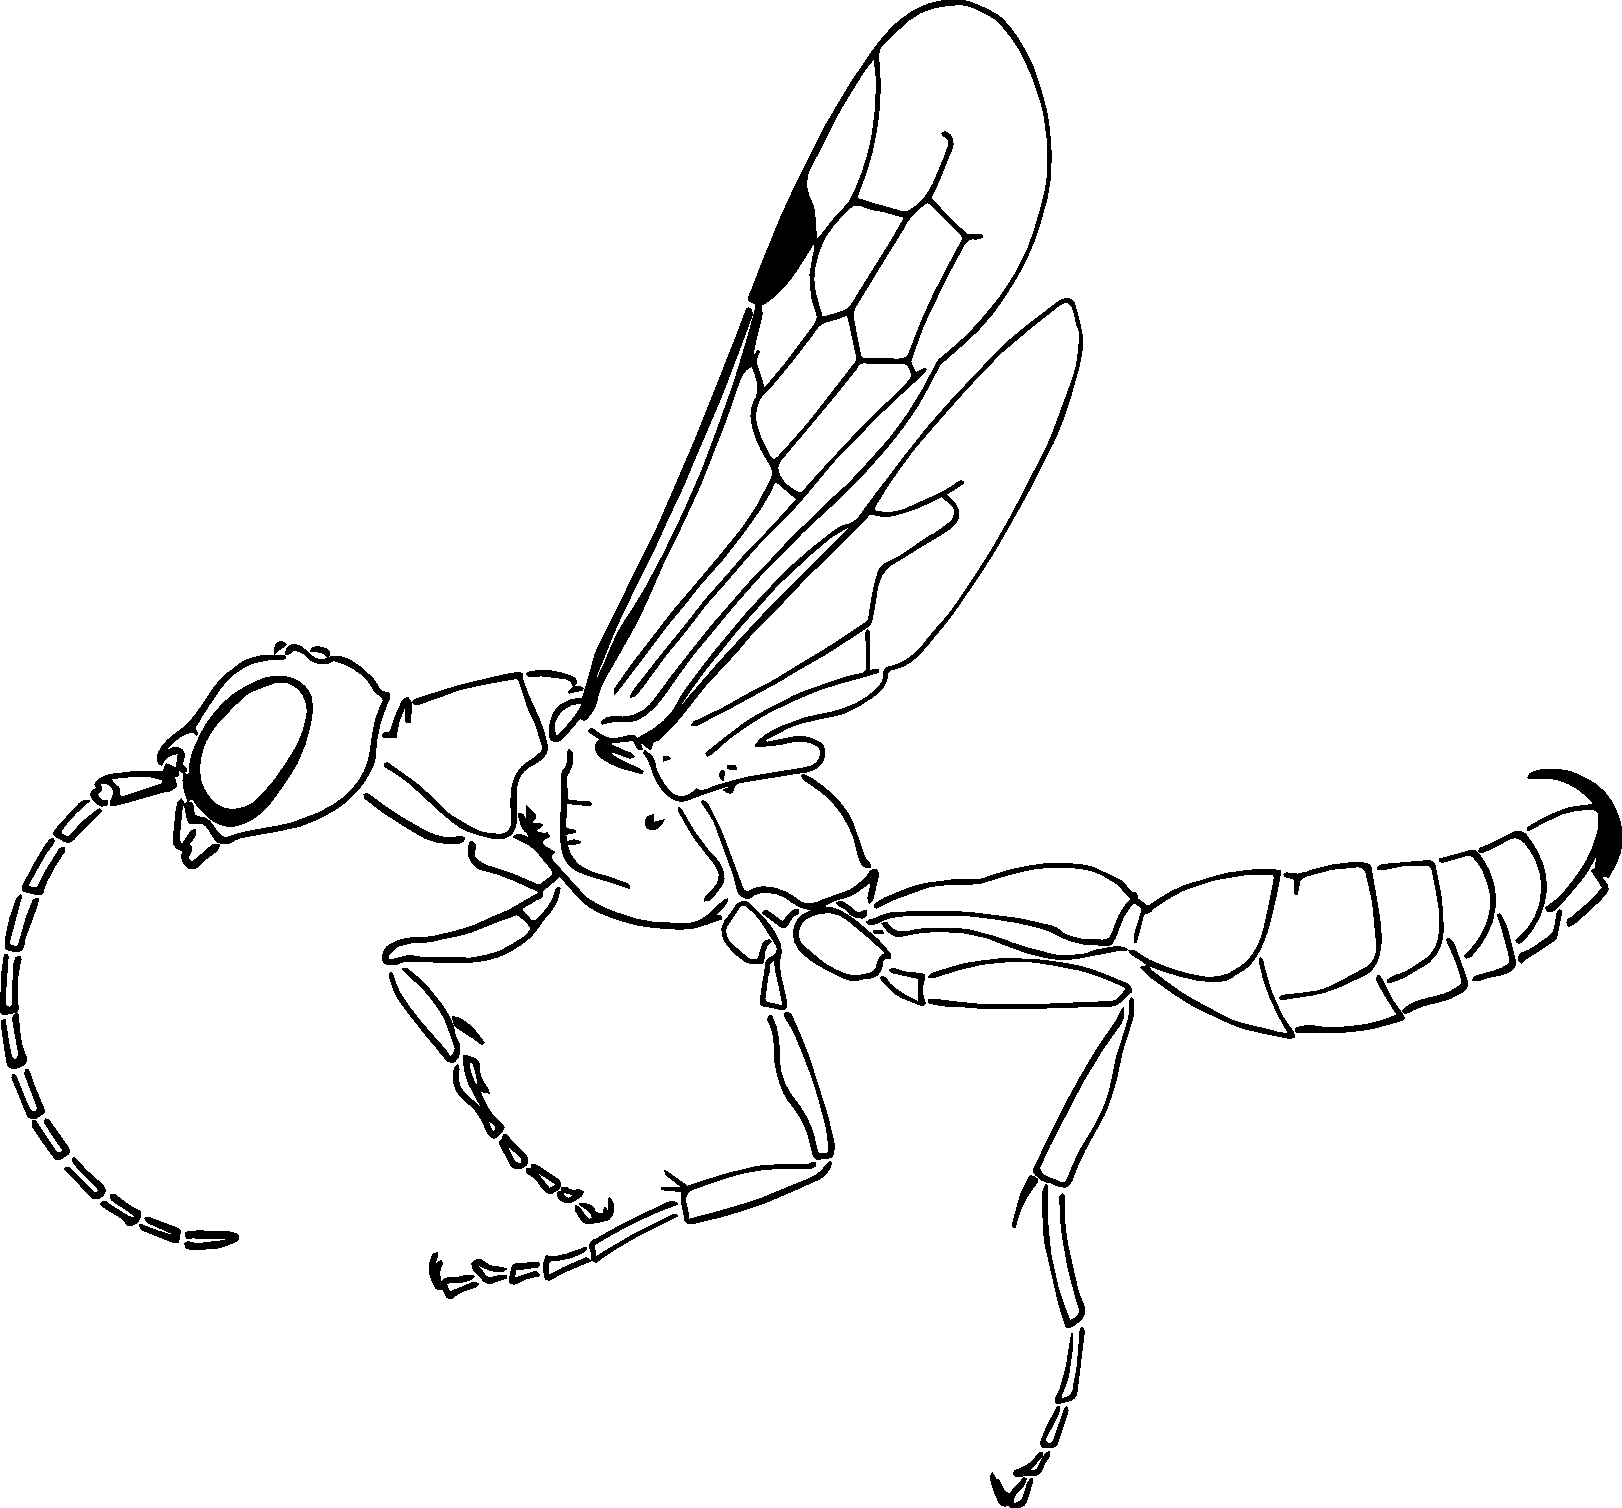
\includegraphics[width=\textwidth]{hymenoptera/TiphiidHabitus}}
        \caption{}
        \label{fig:tiphiid2}
    \end{subfigure}
    \caption{Tiphiidae. \textbf{(a)} Mesosoma in venral view \citep[][pg. 163]{goulet1993hymenoptera}; cx2 = mesocoxa, cx3=metacoxa; \textbf{(b)} habitus \citep[][Fig. 49]{goulet1993hymenoptera}}\label{fig:tiphiidae}
\end{figure}

\subsubsection{Mutillidae (velvet ants)}\index{Mutillidae}
\noindent{}\textit{Diagnostic characters:} metasomal segment 1 without a true node; metasomal segment 2 usually with longitudinal felt line or with felted pit on tergum and/or sternum (but sometimes without); female almost always apterous (figure \ref{fig:mutillid1}); apterous forms with pronotum usually fused to mesothorax and mesonotum to metanotum-propodeum complex; usually very furry and often colorful or brownish and quite ``bristly''; body often very hard and difficult to pin.\vspace{3mm}

\begin{theo}
{}What can you hypothesize about their natural history, given your observations of their phenotypes? Why are velvet ants typically brightly colored?
\end{theo}

\begin{figure}[ht!]
    \centering
    \begin{subfigure}[ht!]{0.45\textwidth}
        \reflectbox{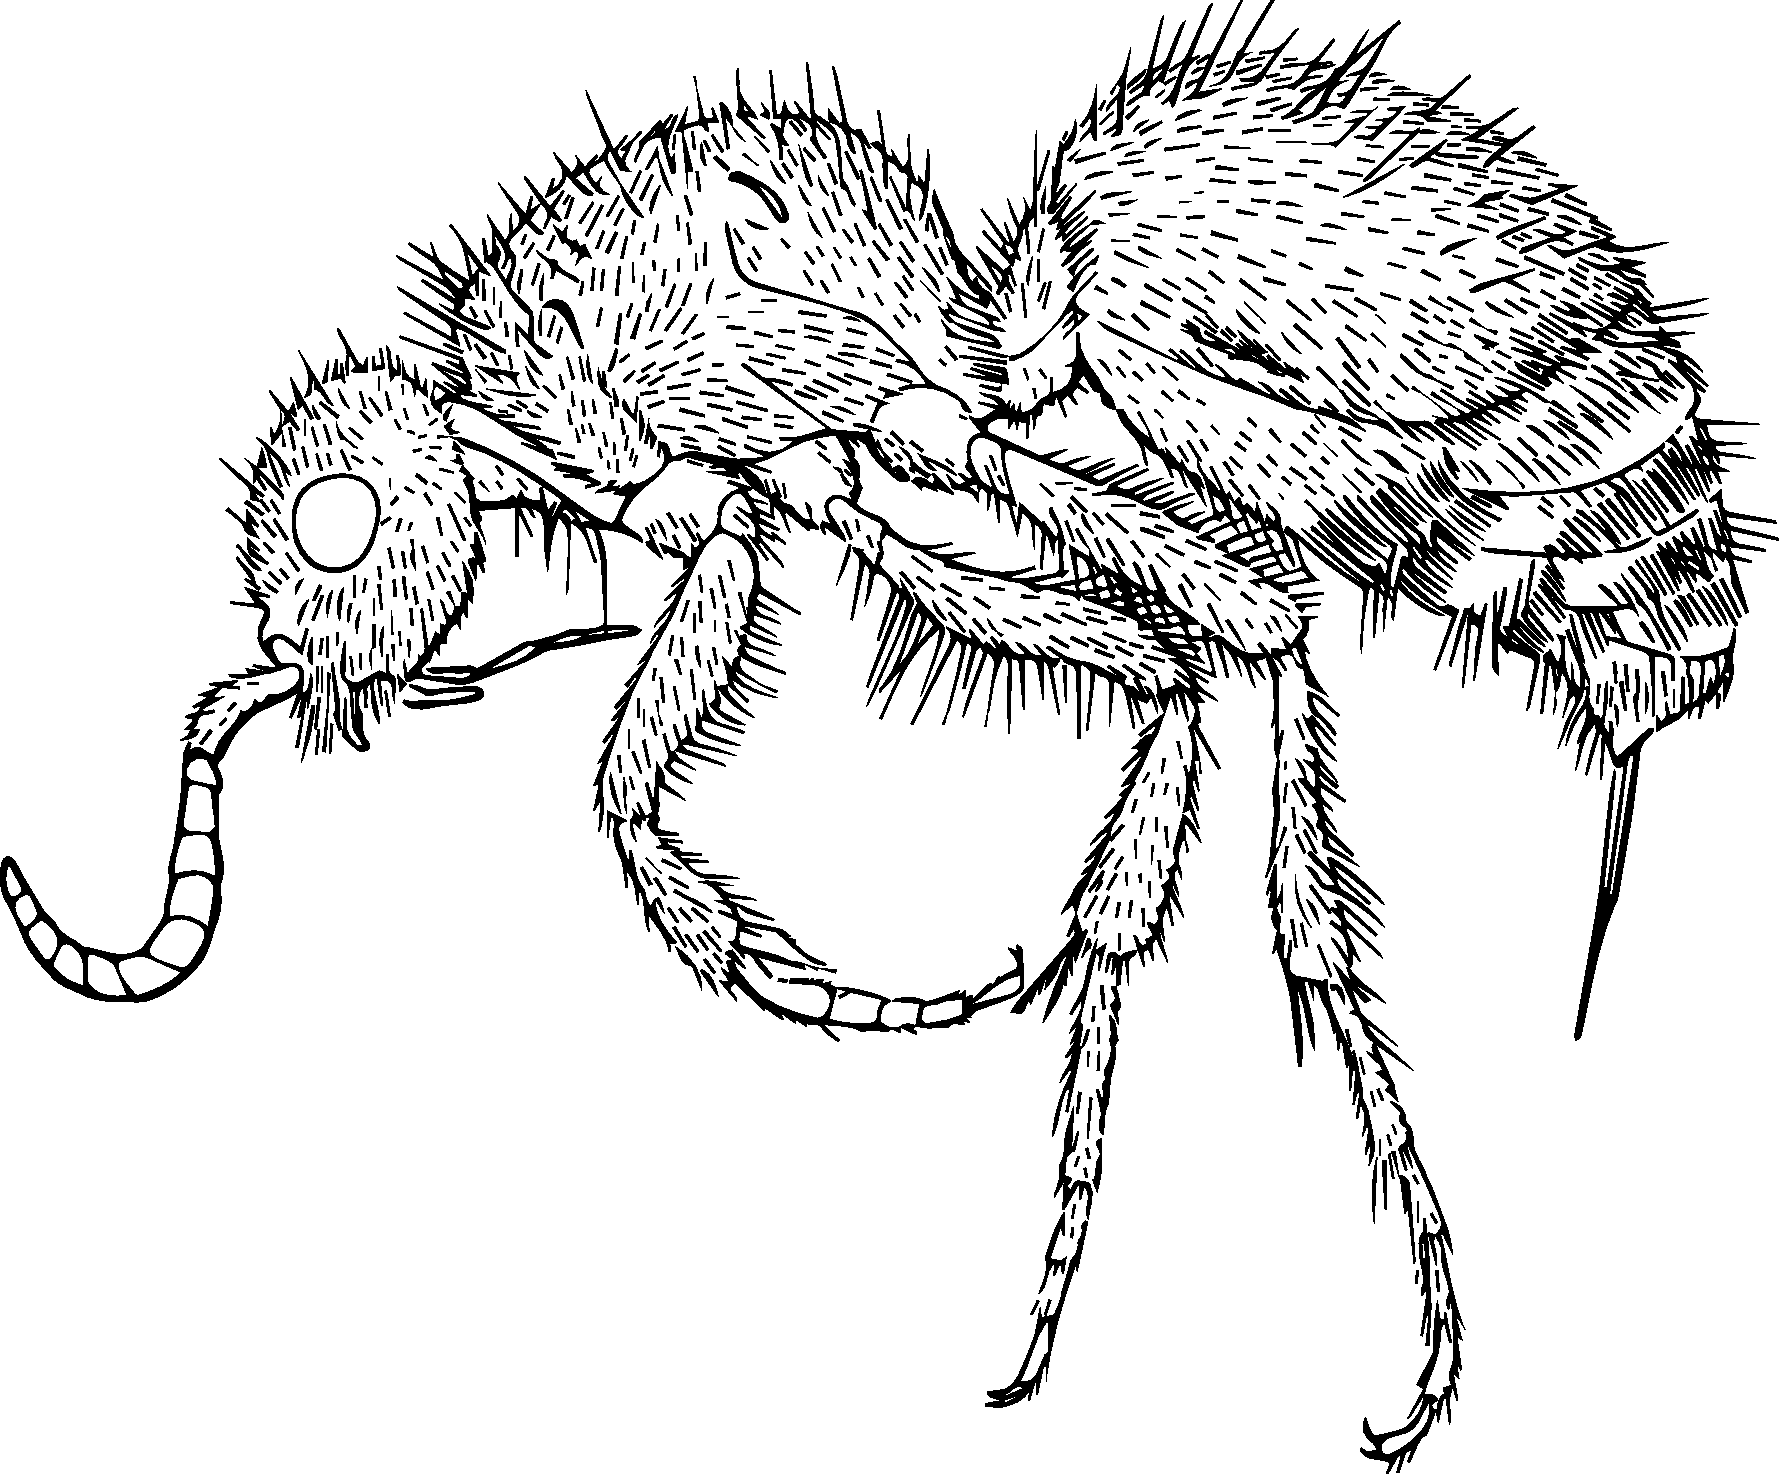
\includegraphics[width=\textwidth]{hymenoptera/MutillidHabitus}}
        \caption{}
        \label{fig:mutillid1}
    \end{subfigure}
    \qquad
    \begin{subfigure}[ht!]{0.42\textwidth}
        \reflectbox{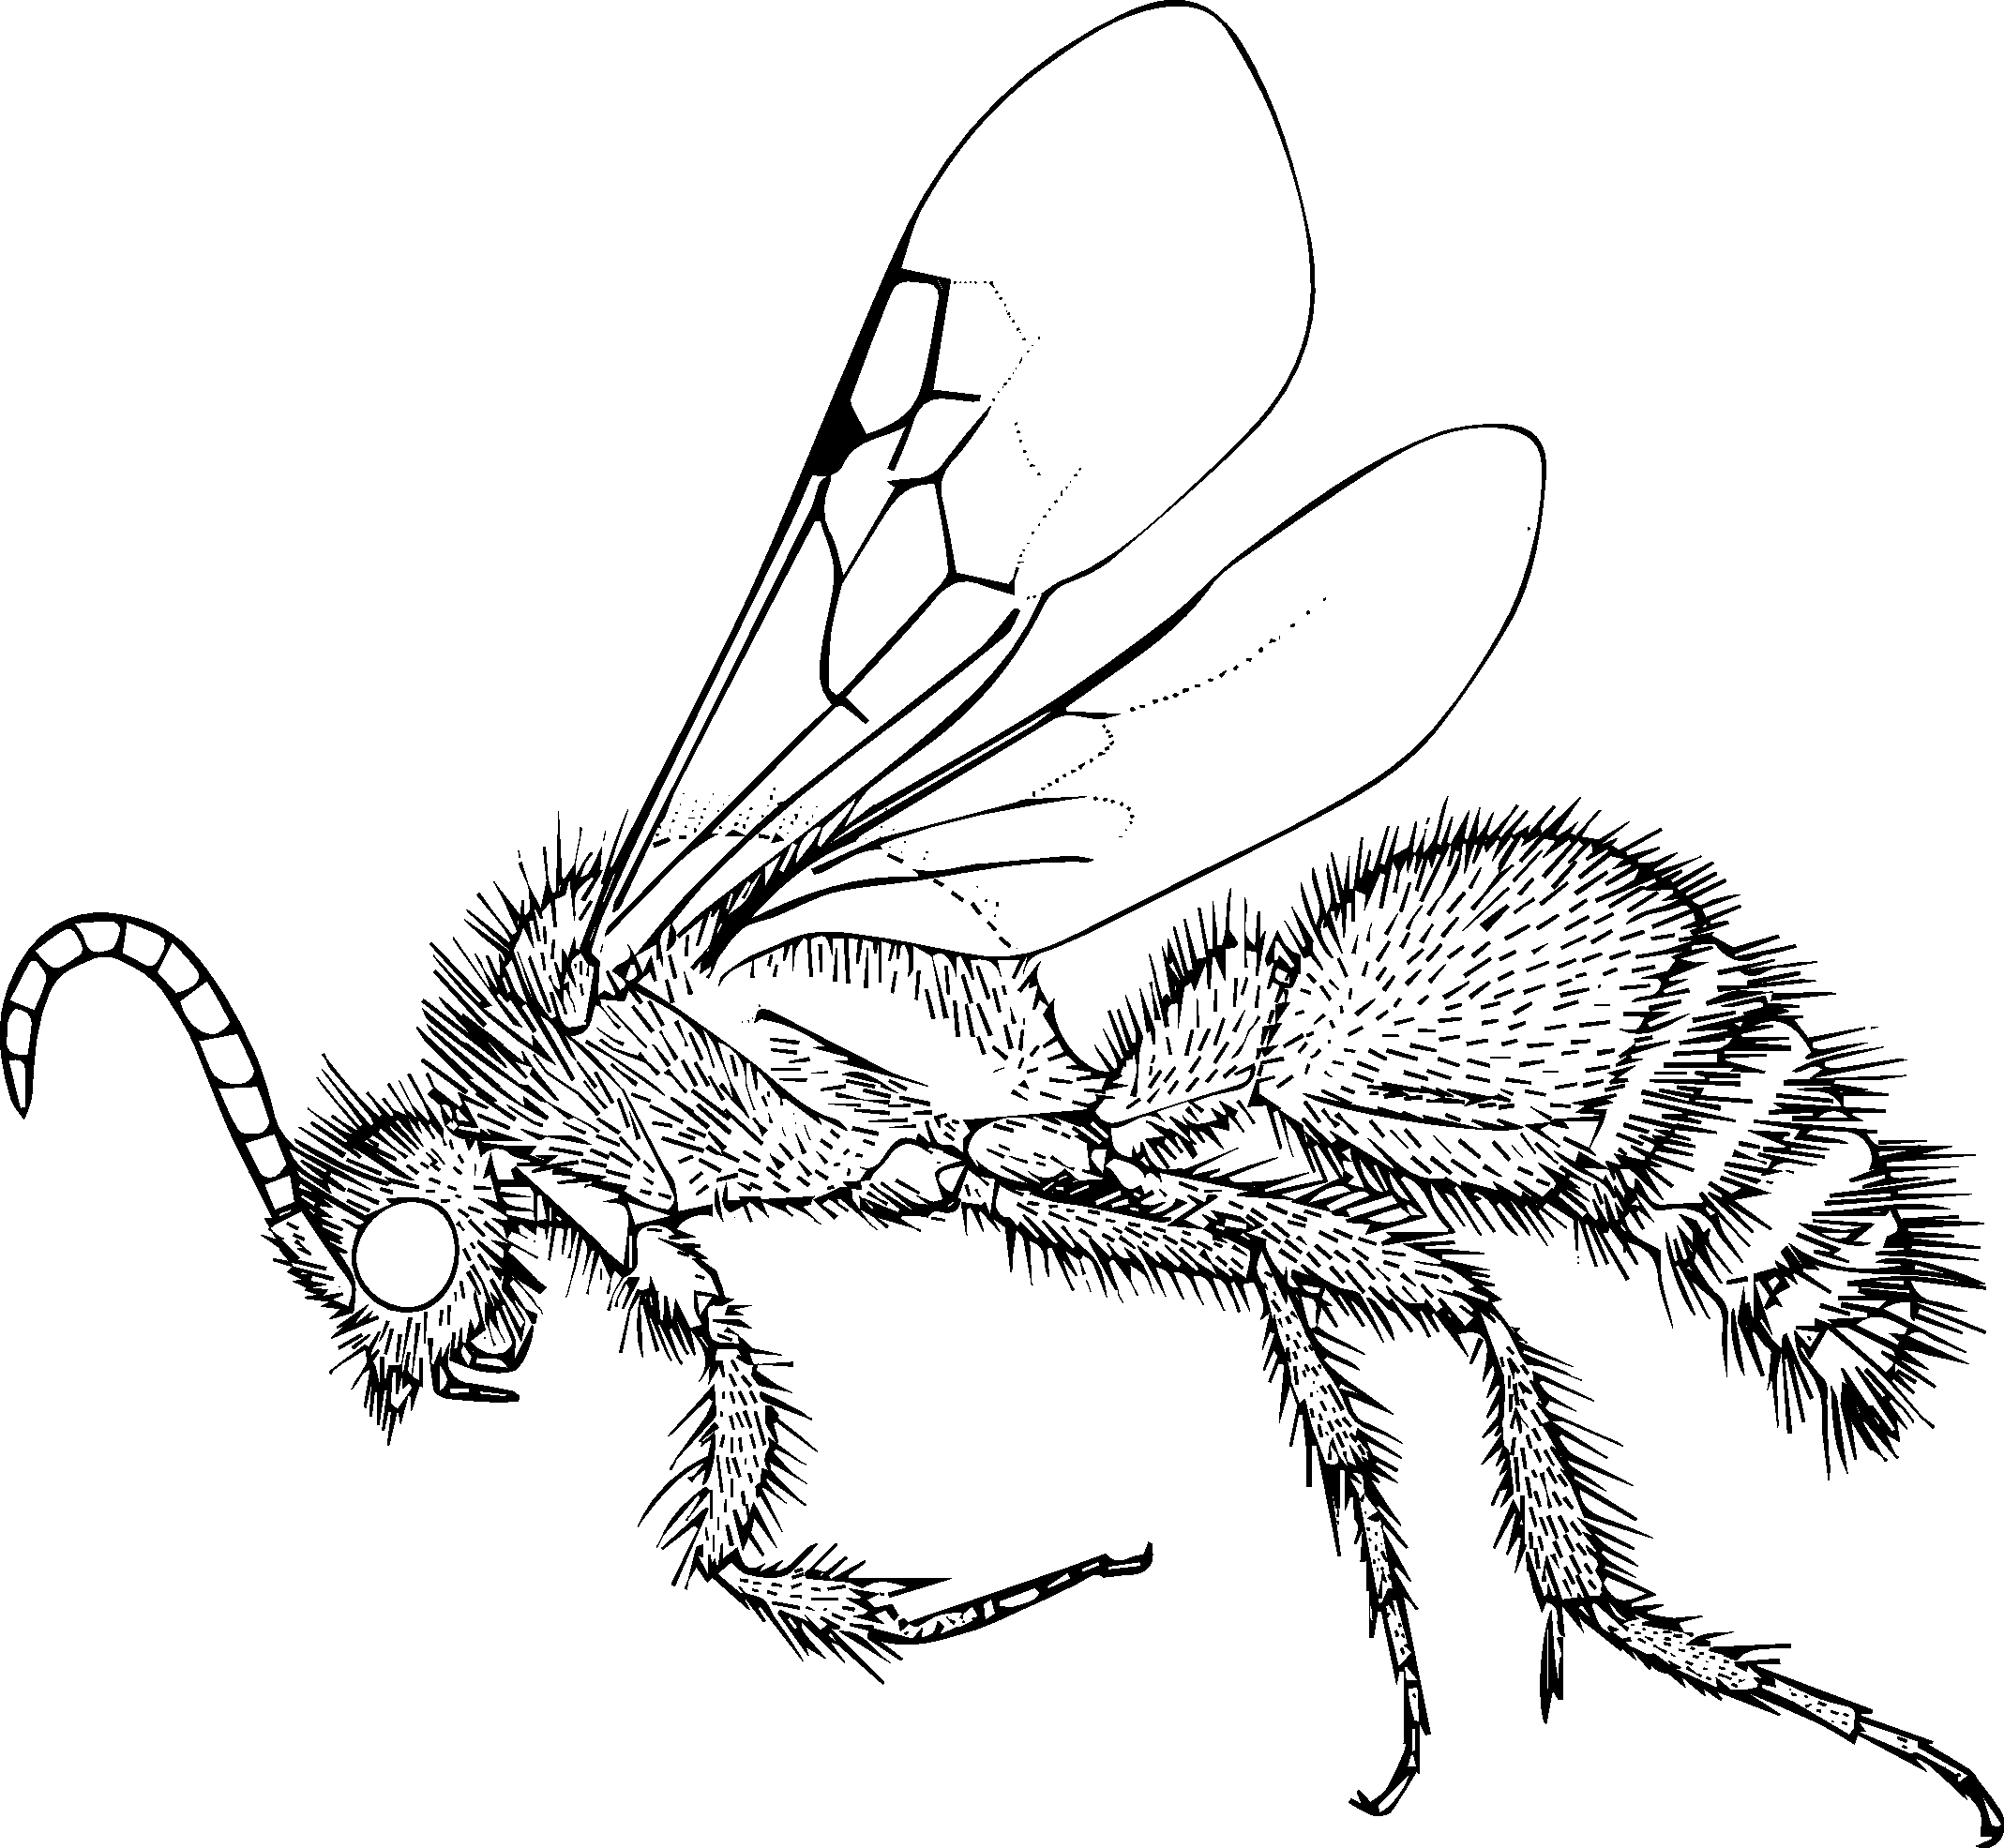
\includegraphics[width=\textwidth]{hymenoptera/MaleMutillidHabitus}}
        \caption{}
        \label{fig:mutillid2}
    \end{subfigure}
    \caption{Mutillidae. \textbf{(a)} Female habitus \citep[][Fig. 63]{goulet1993hymenoptera}; \textbf{(b)} male habitus \citep[][Fig. 64]{goulet1993hymenoptera}}\label{fig:mutillids}
\end{figure}

\subsubsection{Formicidae (ants)}\index{Formicidae}
\noindent{}\textit{Diagnostic characters:} Metapleural gland present (in most species), its opening usually distinct; posterior (inner) spur of metatibia modified as a calcar; reproductive forms usually macropterous (figure \ref{fig:formicid2}), sterile female apterous; apterous form with with pronotum usually freely articulating but sometimes fused with mesothorax; mesonotum and metathorax-propodeum complex usually fused (figure \ref{fig:formicid1}; metasoma petiolate; metasomal segment 1 usually strongly constricted at each end, forming a true node; metasomal sternum 1 separated from sternum 2 by a deep constriction.\vspace{3mm}

\noindent{}\textit{Natural history:} Highly eusocial insects, with a wide array of life history strategies (small \textit{vs}. large colonies, diet specializations, \textit{etc}.) There are $\sim$15,000 species known worldwide.\vspace{3mm}

\begin{theo}
{}Do you see any morphological evidence that ants are highly eusocial? Remember the three main conditions of eusociality ...
\end{theo}

\begin{figure}[ht]
    \centering
    \begin{subfigure}[ht!]{0.42\textwidth}
        \reflectbox{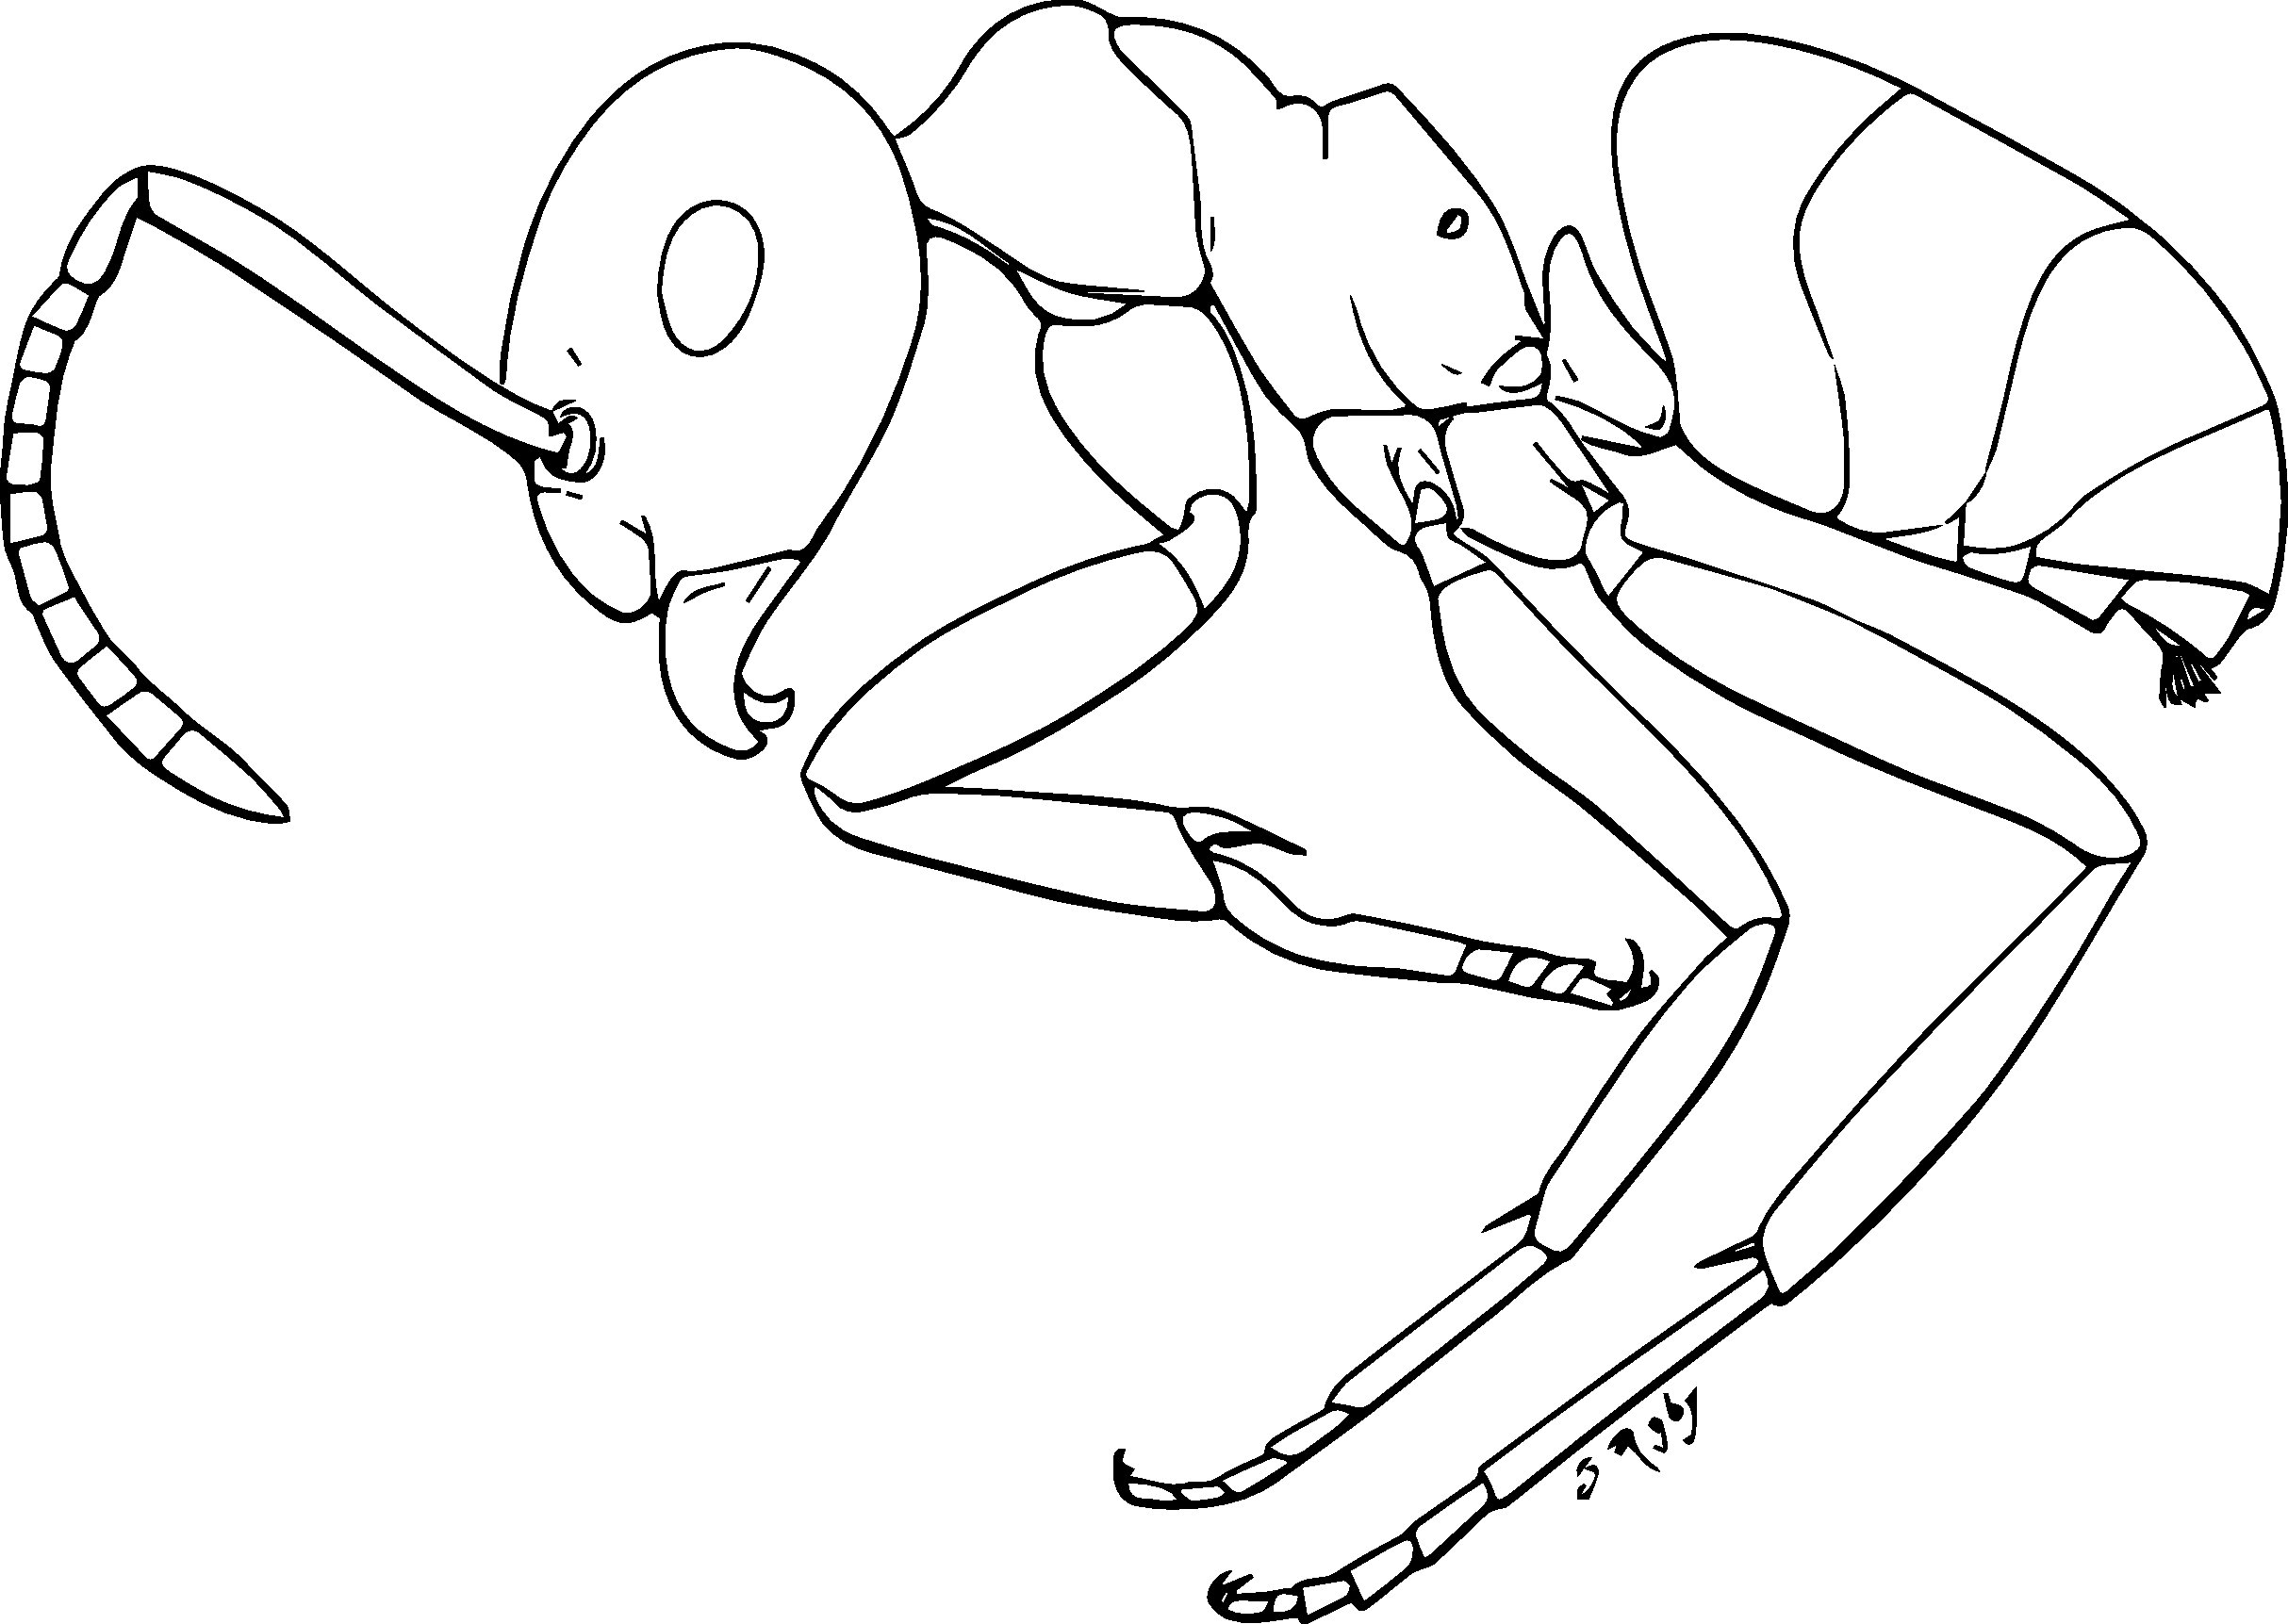
\includegraphics[width=\textwidth]{hymenoptera/FemaleFormicidHabitus}}
        \caption{}
        \label{fig:formicid1}
    \end{subfigure}
    \qquad
    \begin{subfigure}[ht!]{0.3\textwidth}
        \reflectbox{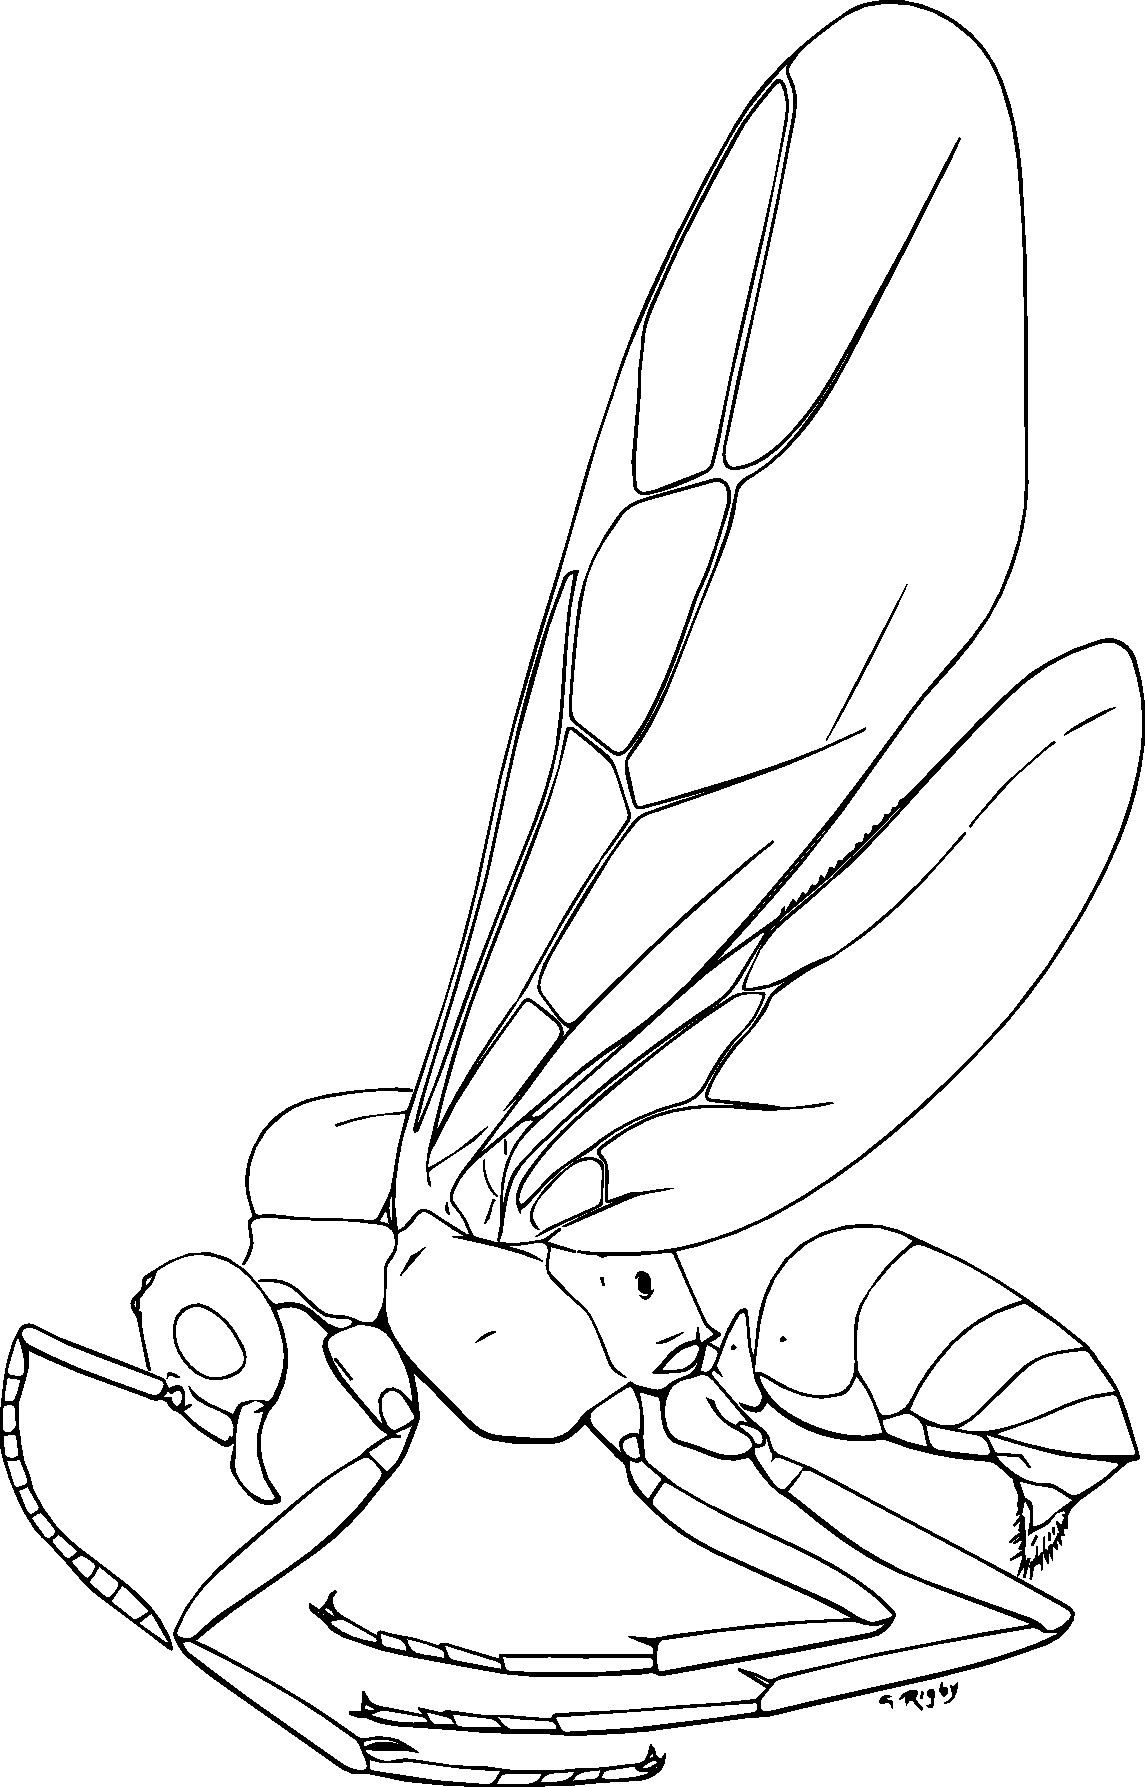
\includegraphics[width=\textwidth]{hymenoptera/MaleFormicidHabitus}}
        \caption{}
        \label{fig:formicid2}
    \end{subfigure}
    \caption{Formicidae. \textbf{(a)} Female habitus \citep[][Fig. 91]{goulet1993hymenoptera}; \textbf{(b)} male habitus \citep[][Fig. 92]{goulet1993hymenoptera}}\label{fig:formicids}
\end{figure}

\subsubsection{Pompilidae (spider wasps)}\index{Pompilidae}
\noindent{}\textit{Diagnostic characters:} Antennal segments distinctly separated and often curled in dead specimens; pronotum with posterolateral apex rounded anterior to tegula; mesopleuron usually with oblique sulcus (figure \ref{fig:pompilid2}); mesosoma usually laterally flattened (\textit{i.e.}, mesosoma higher than wide in anterior or posterior view); hind wing without distinct claval lobe but with distinct jugal lobe (figure \ref{fig:pompilid3}); legs usually conspicuously elongate, spiny.\vspace{3mm}

\noindent{}\textit{Natural history:} Larvae develop as parasitoids of spiders or as cleptoparasites of other pompilids. The spiders are usually paralyzed and brought to a nest (\textit{e.g.}, a mud pot or a burrow in the soil), prior to oviposition. At least 4,200 species are known worldwide.

\begin{figure}[ht]
    \centering
    \begin{subfigure}[ht!]{0.32\textwidth}
        \reflectbox{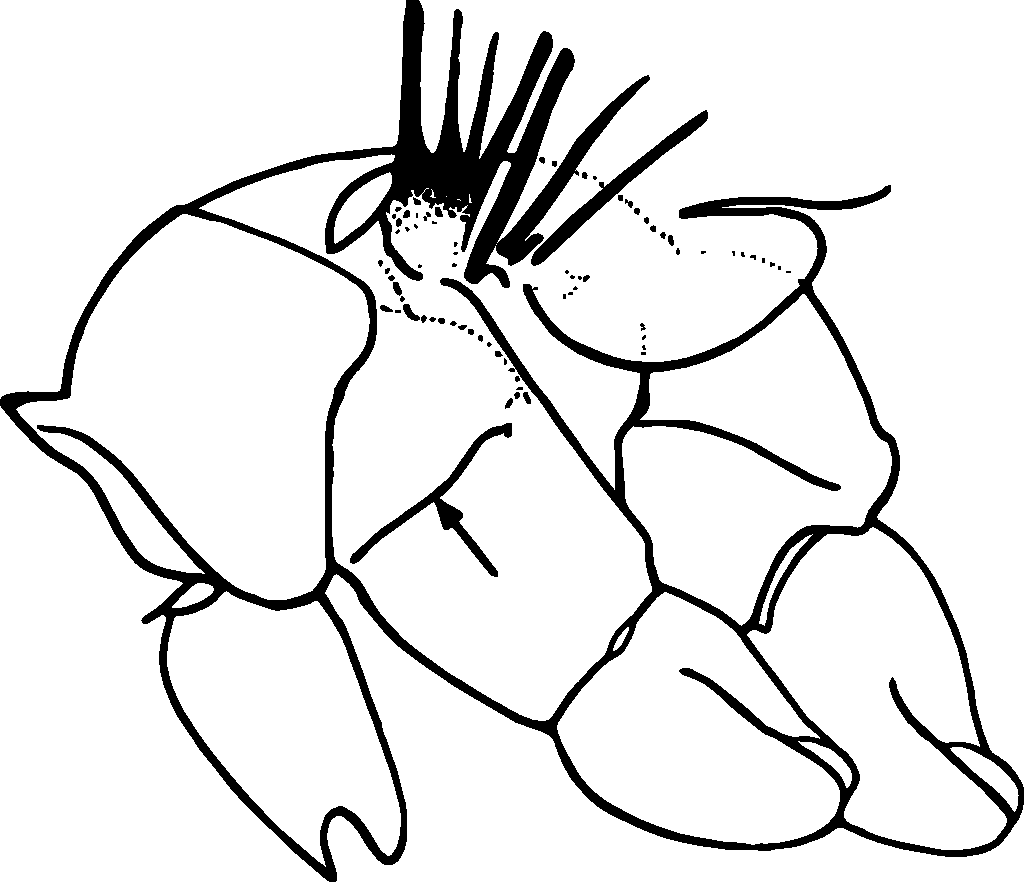
\includegraphics[width=\textwidth]{hymenoptera/PompilidMesosoma}}
        \caption{}
        \label{fig:pompilid2}
    \end{subfigure}
    \qquad
    \begin{subfigure}[ht!]{0.38\textwidth}
        \reflectbox{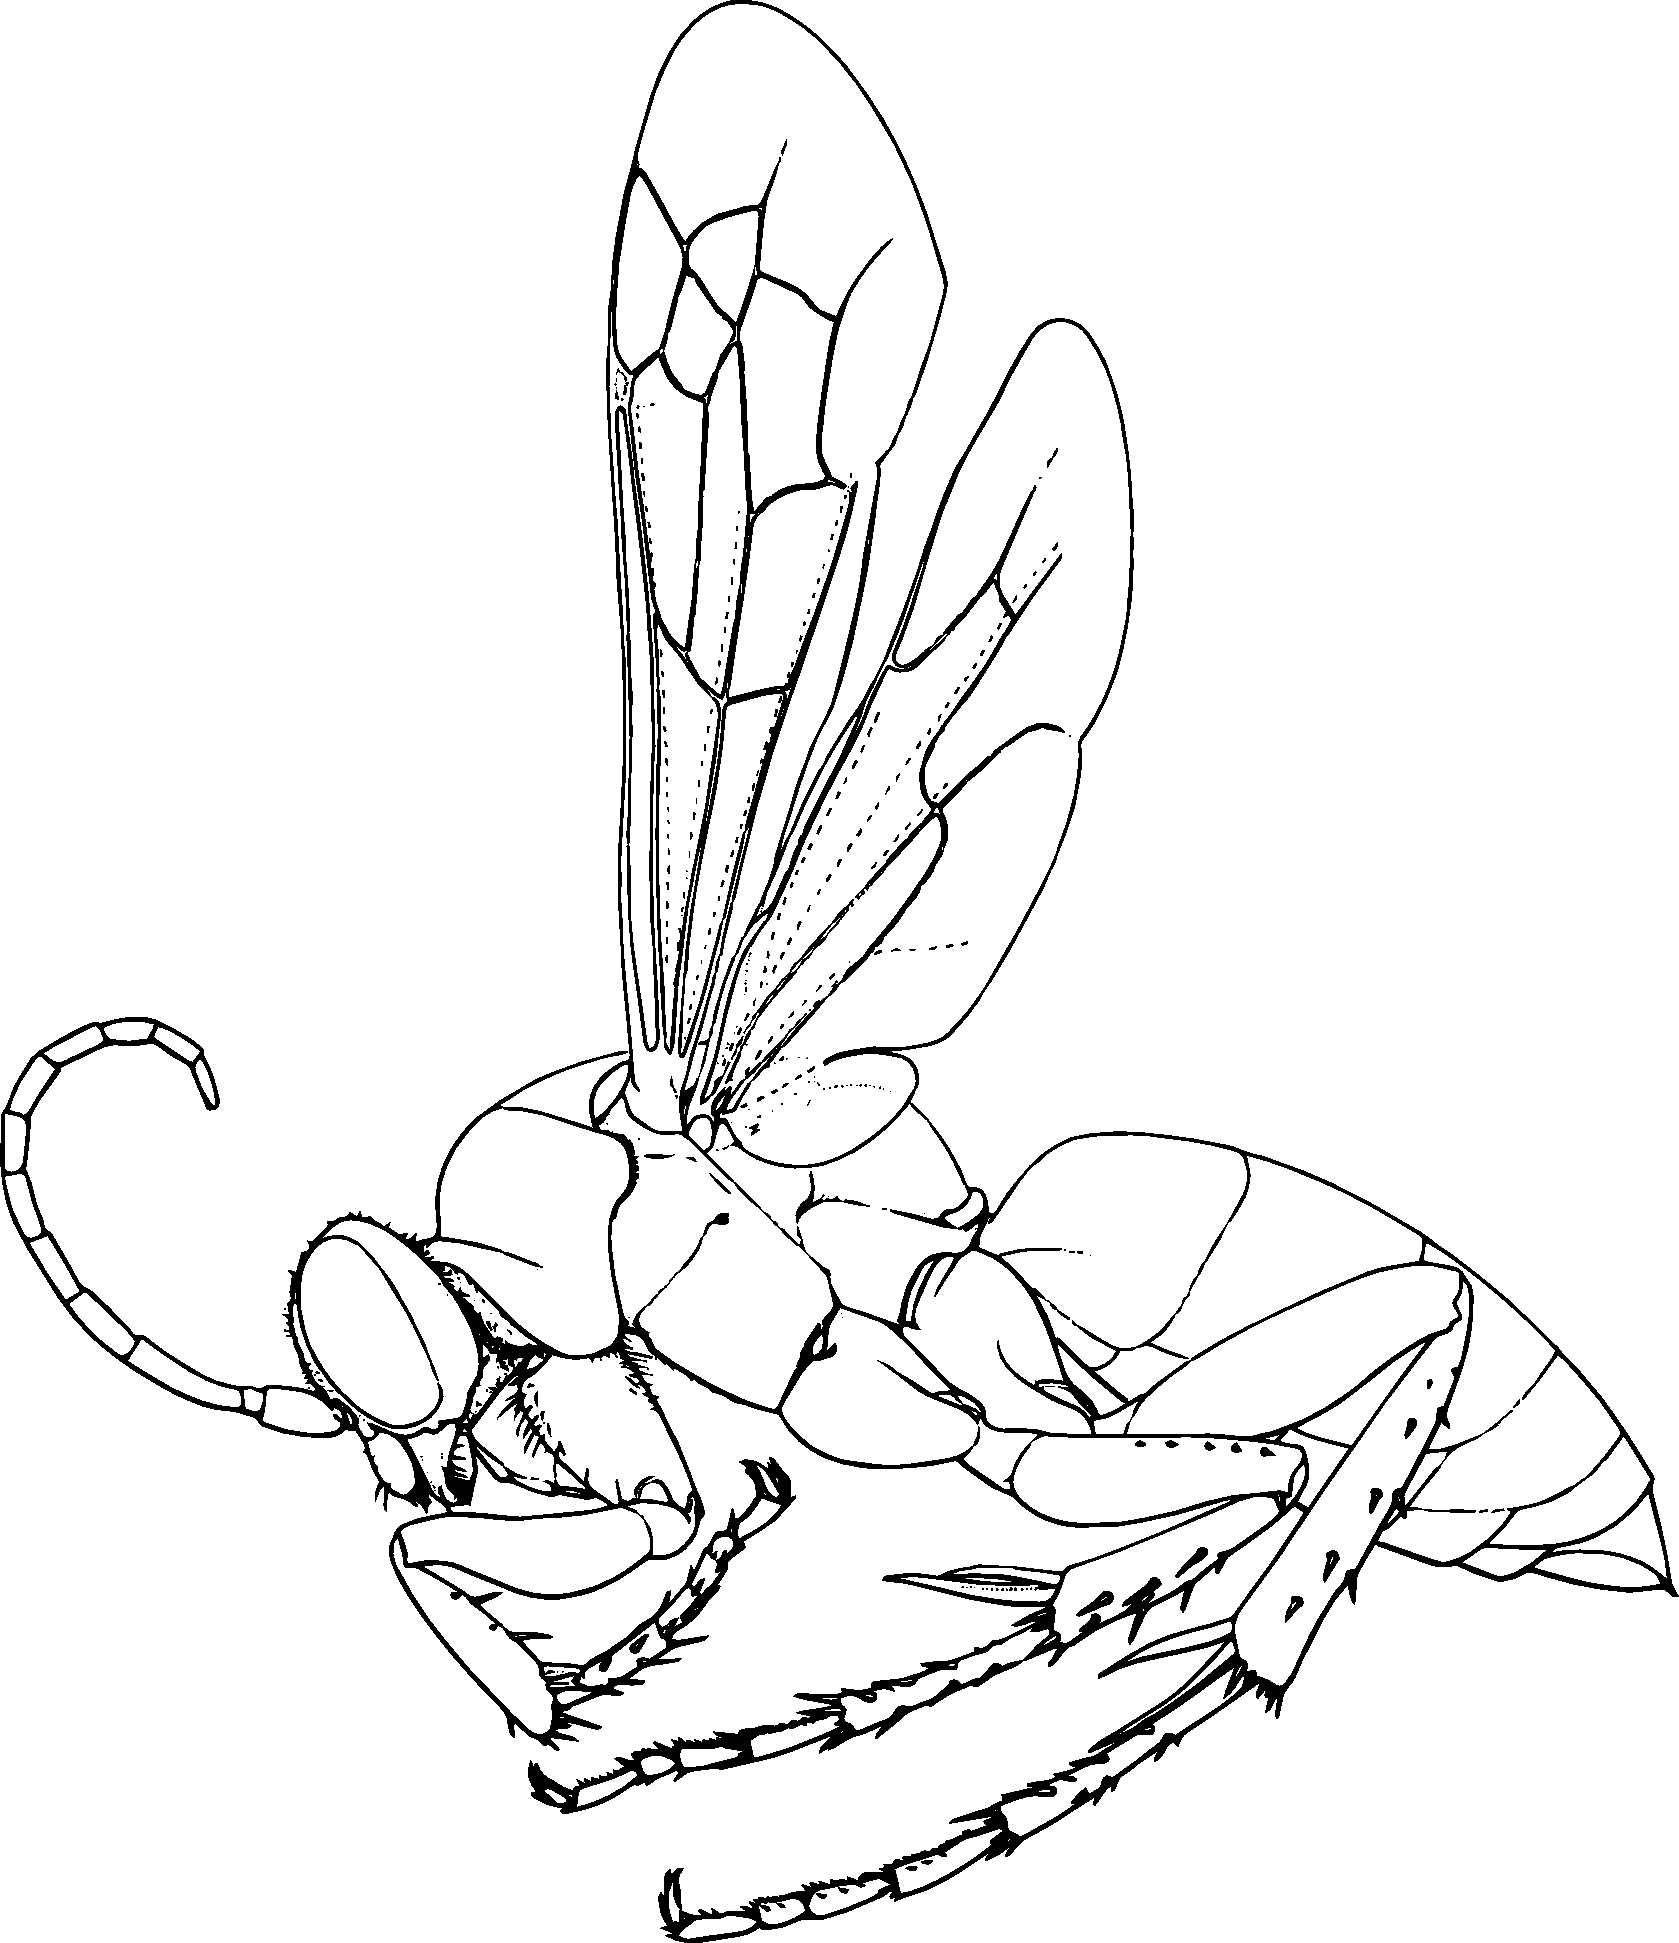
\includegraphics[width=\textwidth]{hymenoptera/PompilidHabitus}}
        \caption{}
        \label{fig:pompilid3}
    \end{subfigure}
    \caption{Pompilidae. \textbf{(a)} Mesosoma, with mesopleural sulcus (arrow) \citep[][pg. 170]{goulet1993hymenoptera}; \textbf{(b)} Habitus \citep[][Fig. 71]{goulet1993hymenoptera}}\label{fig:pompilid}
\end{figure}

\subsubsection{Scoliidae}\index{Scoliidae}
\noindent{}\textit{Diagnostic characters:} Eye with inner margin deeply emarginated (``notched''); pronotum with posterodorsal margin U-shaped; mesocoxae and metacoxa widely separated; wings with dense fine longitudinal wrinkles near apices (figure \ref{fig:scoliid1}); hind wing without distinct claval lobe but with distinct jugal lobe; female usually with mesotibia and metatibia stout and spiny; metasomal sternum 1 separated from sternum 2 by a deep constriction.\\

\noindent{}\textit{Natural history:} Based on rearing records, most of the $\sim$300 described species are predicted to be ectoparasitoids of Coleoptera larvae, especially Scarabaeoidea.

\begin{figure}[ht!]
    \centering
    \begin{subfigure}[ht!]{0.28\textwidth}
        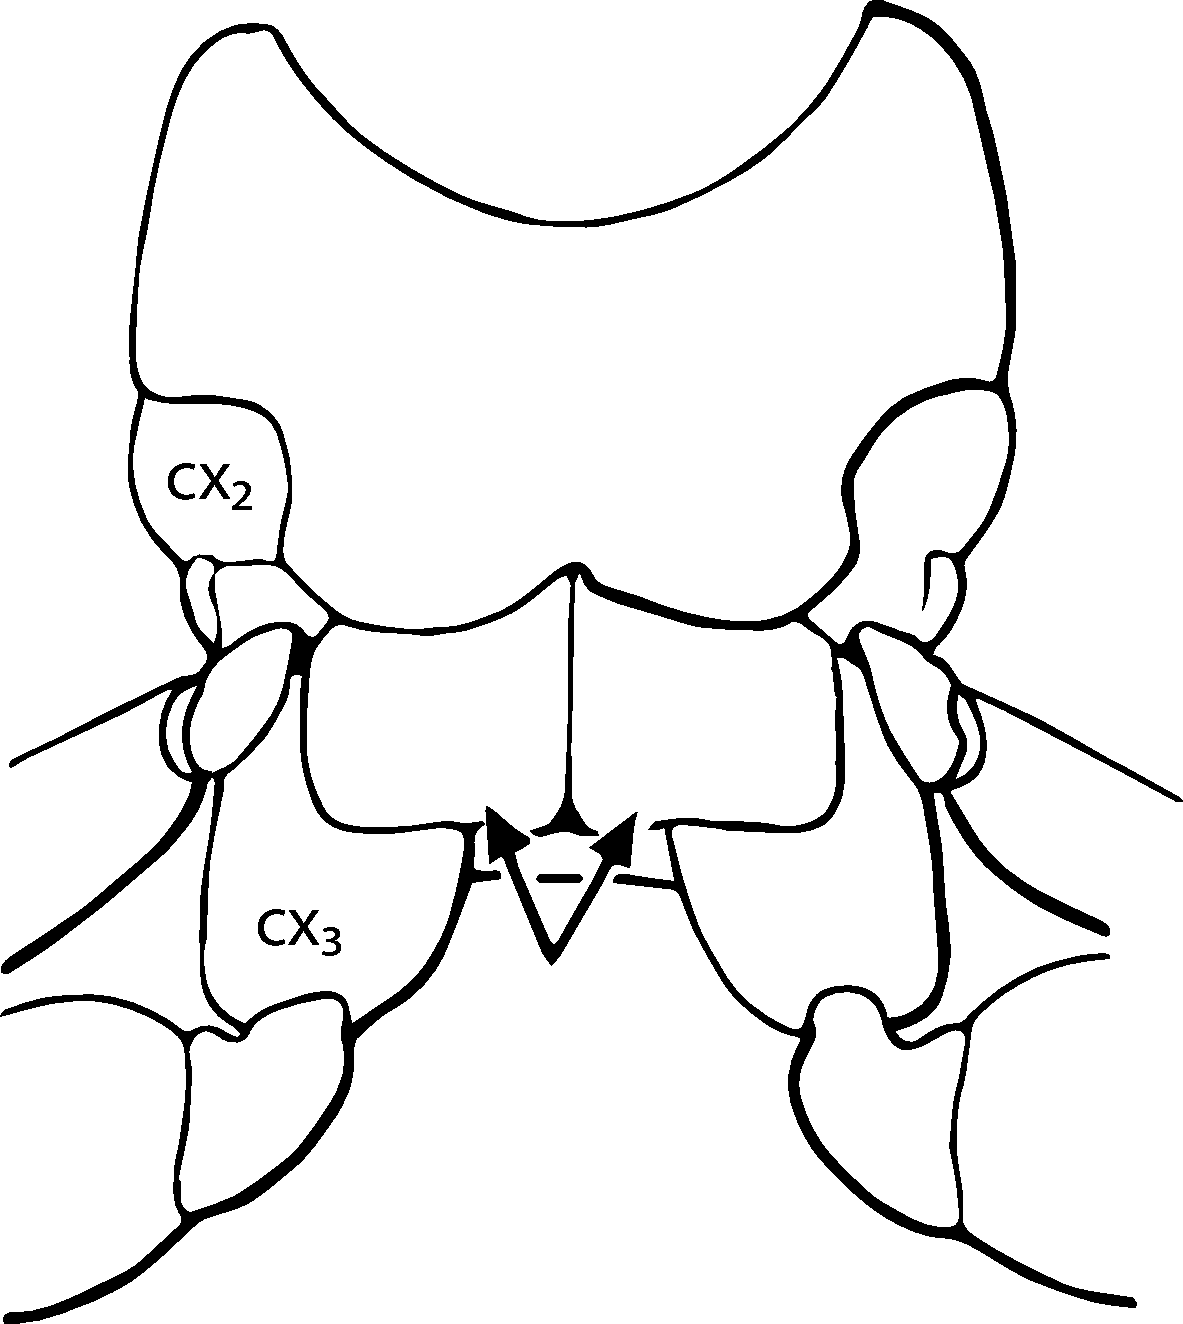
\includegraphics[width=\textwidth]{hymenoptera/ScoliidMesosoma}
        \caption{}
        \label{fig:scoliid1}
    \end{subfigure}
    \qquad
    \begin{subfigure}[ht!]{0.38\textwidth}
        \reflectbox{\includegraphics[width=\textwidth]{hymenoptera/ScoliidHabitus}}
        \caption{}
        \label{fig:scoliid2}
    \end{subfigure}
    \caption{Scoliidae. \textbf{(a)} Mesosoma in ventral view \citep[][pg. 162]{goulet1993hymenoptera}; cx3 = metacoxa; \textbf{(b)} habitus \citep[][Fig. 78]{goulet1993hymenoptera}}\label{fig:scoliids}
\end{figure}

\subsubsection{Vespidae (hornets, paper wasps, pollen wasps, potter wasps, \textit{etc}.)}\index{Vespidae}
\noindent{}\textit{Diagnostic characters:} Eye with inner margin deeply emarginated; pronotum posterodorsal margin V-shaped, and with pronotum posterolateral apex acute and strongly produced above anterior margin of tegula; fore wing almost always longitudinally folded when at rest; hind wing without distinct claval lobe, and usually with distinct jugal lobe; posterior (inner) spur of metatibia weakly modified as a calcar; metasomal sternum 1 separated from sternum 2 by a deep constriction.\vspace{3mm}

\noindent{}\textit{Natural history:} With about 4,000 described species, this family exhibits a wide range of behaviors. Many species (\textit{e.g}., Eumeninae) are solitary, while others are highly eusocial (\textit{e.g.}, Vespinae).

\begin{theo}
{}Do you see any morphological evidence that these species are eusocial? Recall the question above for Formicidae.
\end{theo}

\begin{figure}[ht!]
    \centering
    \begin{subfigure}[ht!]{0.22\textwidth}
        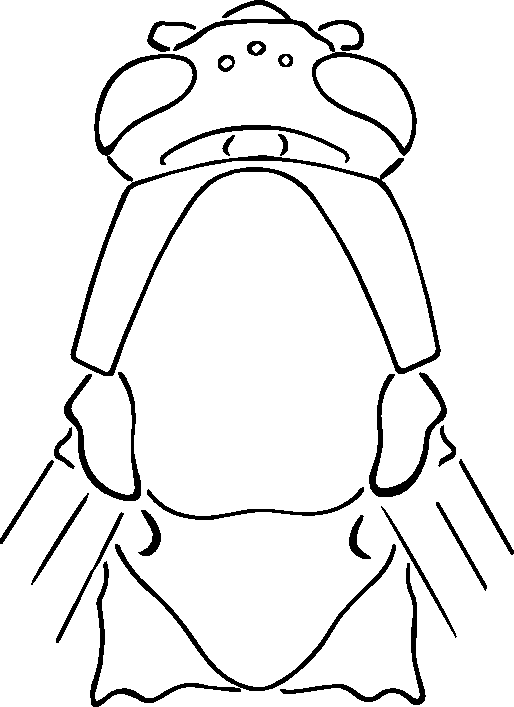
\includegraphics[width=\textwidth]{hymenoptera/VespidMesosoma}
        \caption{}
        \label{fig:vespid1}
    \end{subfigure}
    \hfill
    \begin{subfigure}[ht!]{0.2\textwidth}
        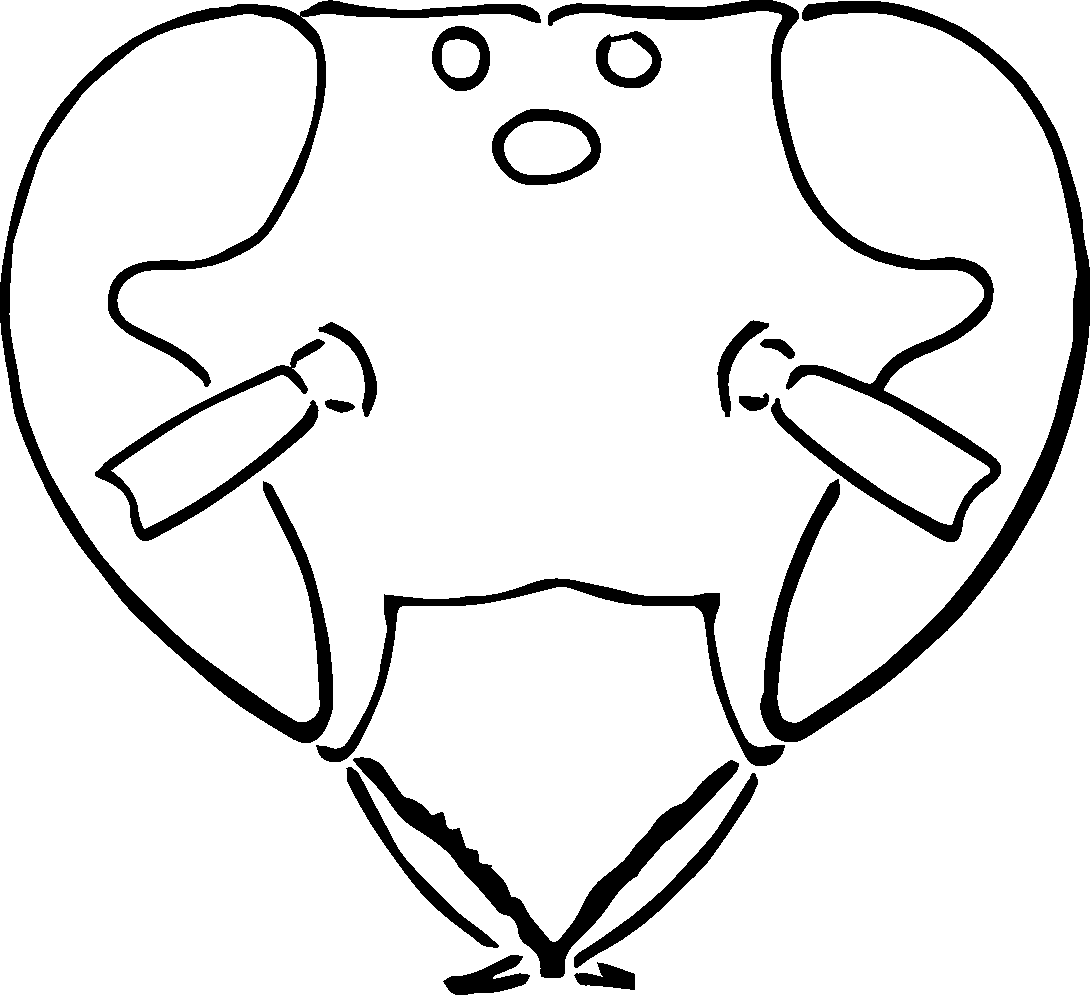
\includegraphics[width=\textwidth]{hymenoptera/VespidHead}
        \caption{}
        \label{fig:vespid2}
    \end{subfigure}
    \hfill
    \begin{subfigure}[ht!]{0.45\textwidth}
        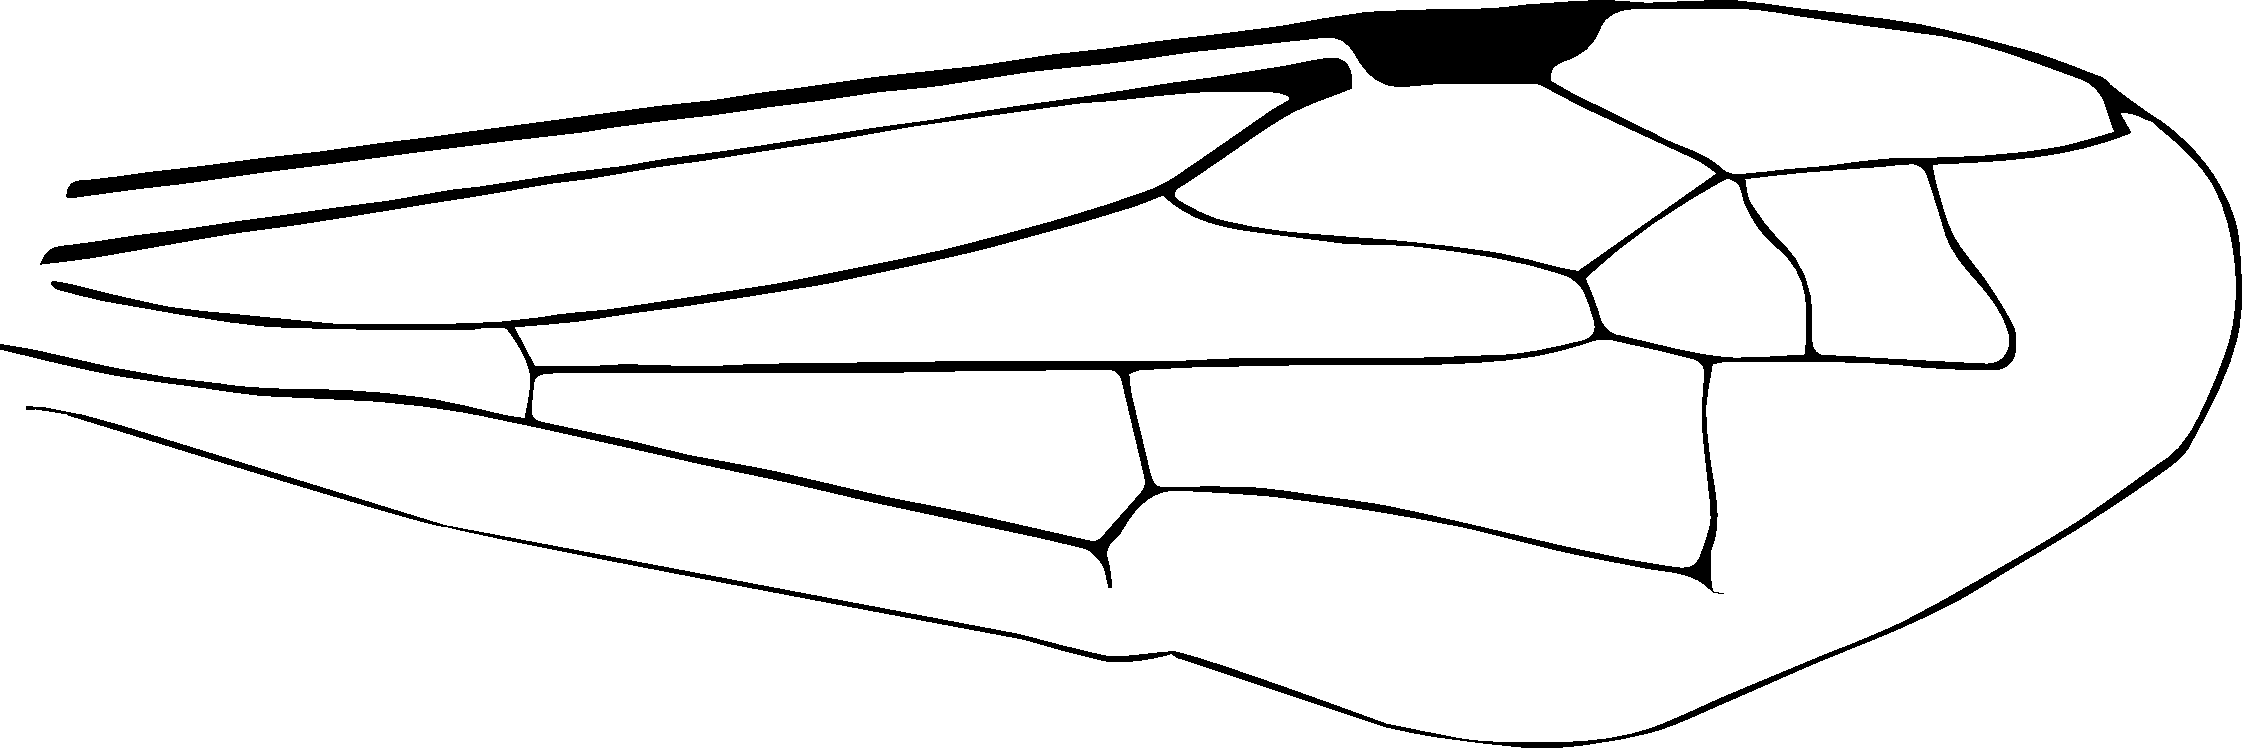
\includegraphics[width=\textwidth]{hymenoptera/VespidWing}
        \caption{}
        \label{fig:vespid3}
    \end{subfigure}
    \caption{Vespidae. \textbf{(a)} Dorsal head and mesosoma; \textbf{(b)} anterior head; \textbf{(c)} fore wing \citep[][pp. 214--215]{goulet1993hymenoptera}}\label{fig:vespids}
\end{figure}
\FloatBarrier

\paragraph*{Apoidea} There are four families of ``spheciform'' wasps (we'll look at two), which are mostly predators of other insects, and seven to nine families of bees (Anthophila; we'll look at four bee families), which collect pollen.\index{Apoidea}\vspace{3mm}

\subsubsection{Sphecidae (thread-waisted, hunting wasps)}\index{Sphecidae}
\noindent{}\textit{Diagnostic characters:} Plumose, branched setae absent; hind leg basitarsus as wide as subsequent tarsomeres; metasoma petiolate (figure \ref{fig:sphecid1}); first metasomal segment tube-like (sternum and tergum fused).\vspace{3mm}

\noindent{}\textit{Natural history:} Females construct nests from mud, use pre-existing cavities, or excavate nests from soil or sand. The nests are selectively provisioned with prey for the larvae to consume during their development. There are almost 800 described species, and they exhibit a range of behaviors from solitary to almost eusocial.

\begin{figure}[ht!]
    \centering
    \begin{subfigure}[ht!]{0.45\textwidth}
        \reflectbox{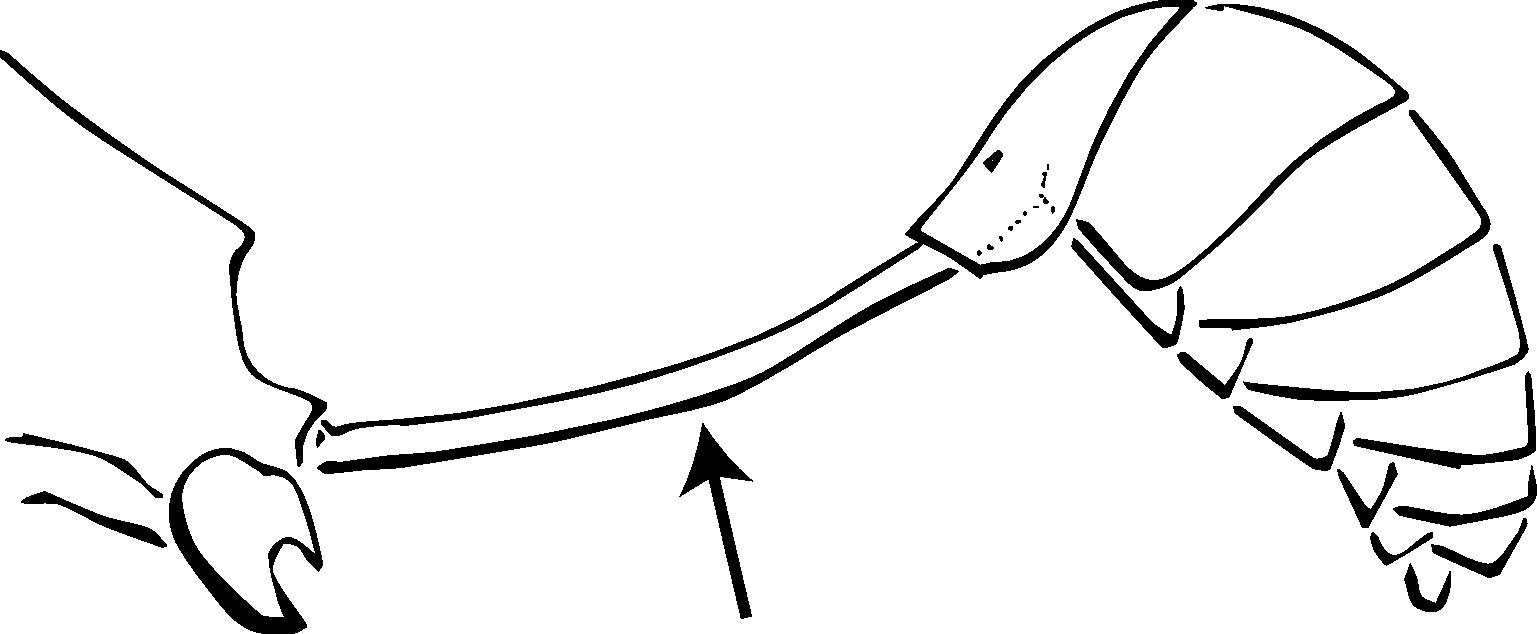
\includegraphics[width=\textwidth]{hymenoptera/SphecidMetasoma}}
        \caption{}
        \label{fig:sphecid1}
    \end{subfigure}
    \qquad
    \begin{subfigure}[ht!]{0.45\textwidth}
        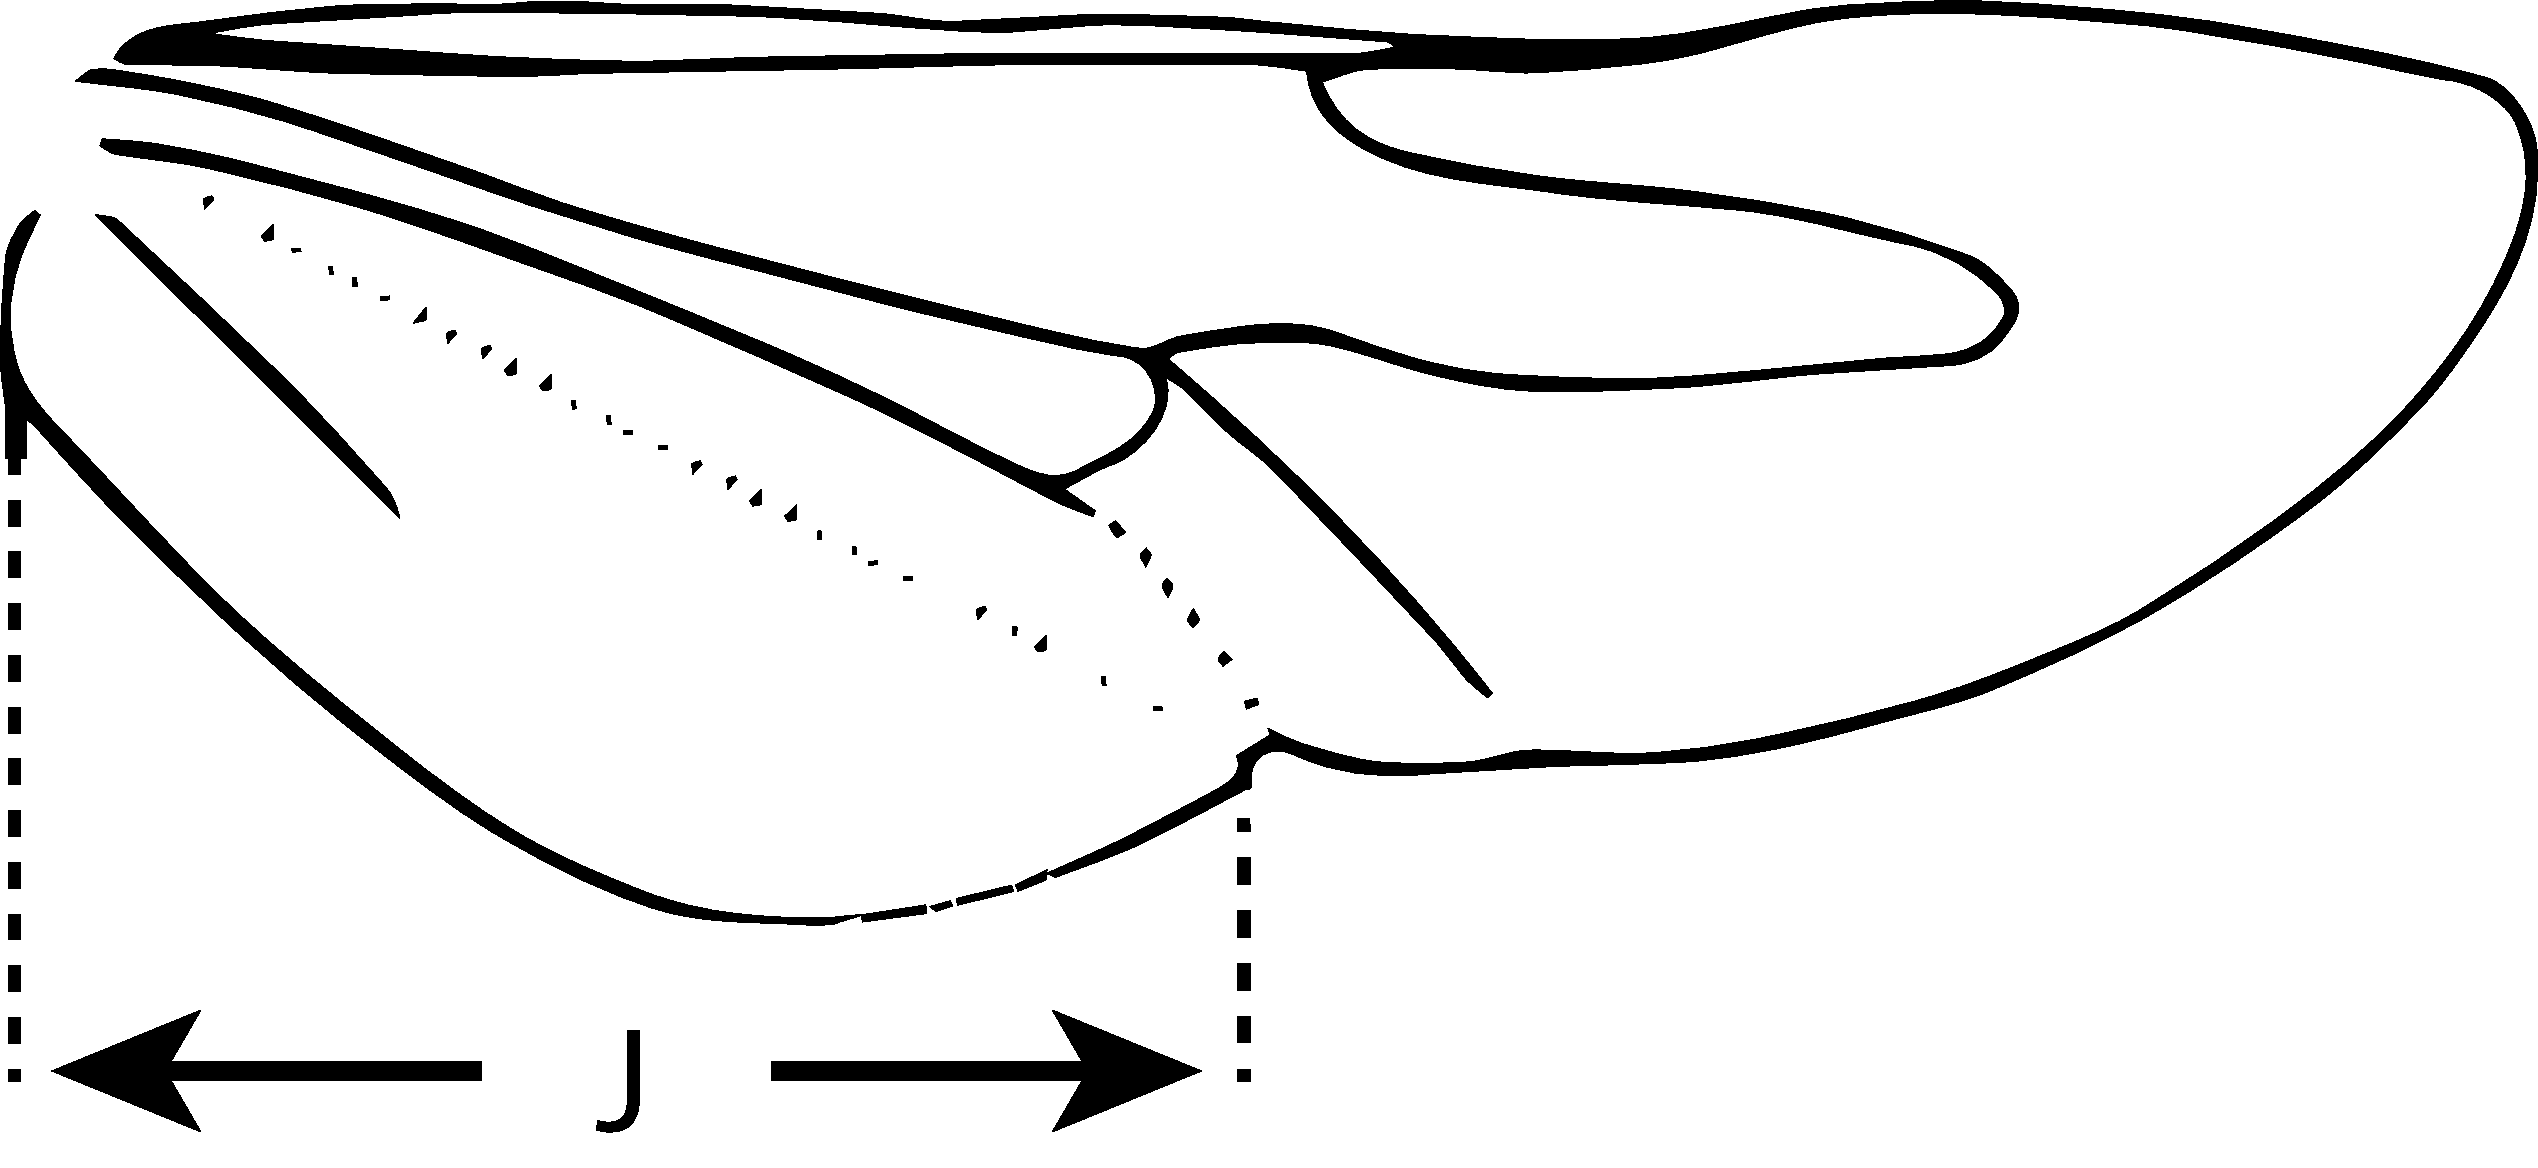
\includegraphics[width=\textwidth]{hymenoptera/SphecidWing}
        \caption{}
        \label{fig:sphecid2}
    \end{subfigure}
    \caption{Sphecidae. \textbf{(a)} Mesasoma; s1 = sternite 1; \textbf{(b)} Hind wing; J = jugal lobe \citep[][pg. 281]{goulet1993hymenoptera}}\label{fig:sphecids}
\end{figure}

\subsubsection{Crabronidae (hunting wasps, aphid wasps, beewolves, cicada killers, \textit{etc}.)}\index{Crabronidae}
\noindent{}\textit{Diagnostic characters:} plumose, branched setae absent; hind leg basitarsus as wide as subsequent tarsomeres; tergum and sternum distinctly separated on metasomal segment 1; sometimes forming tube-like petiole; often determined through the process of elimination.\vspace{3mm}

\noindent{}\textit{Natural history:} This taxon is among the most diverse in Apoidea, with almost 9,000 described species. The limits of this family are still being debated, and it's likely that our concept of Crabronidae is polyphyletic. The nesting behaviors and prey specialization are highly variable.

\begin{figure}[ht!]
    \centering
    \begin{subfigure}[ht!]{0.44\textwidth}
        \reflectbox{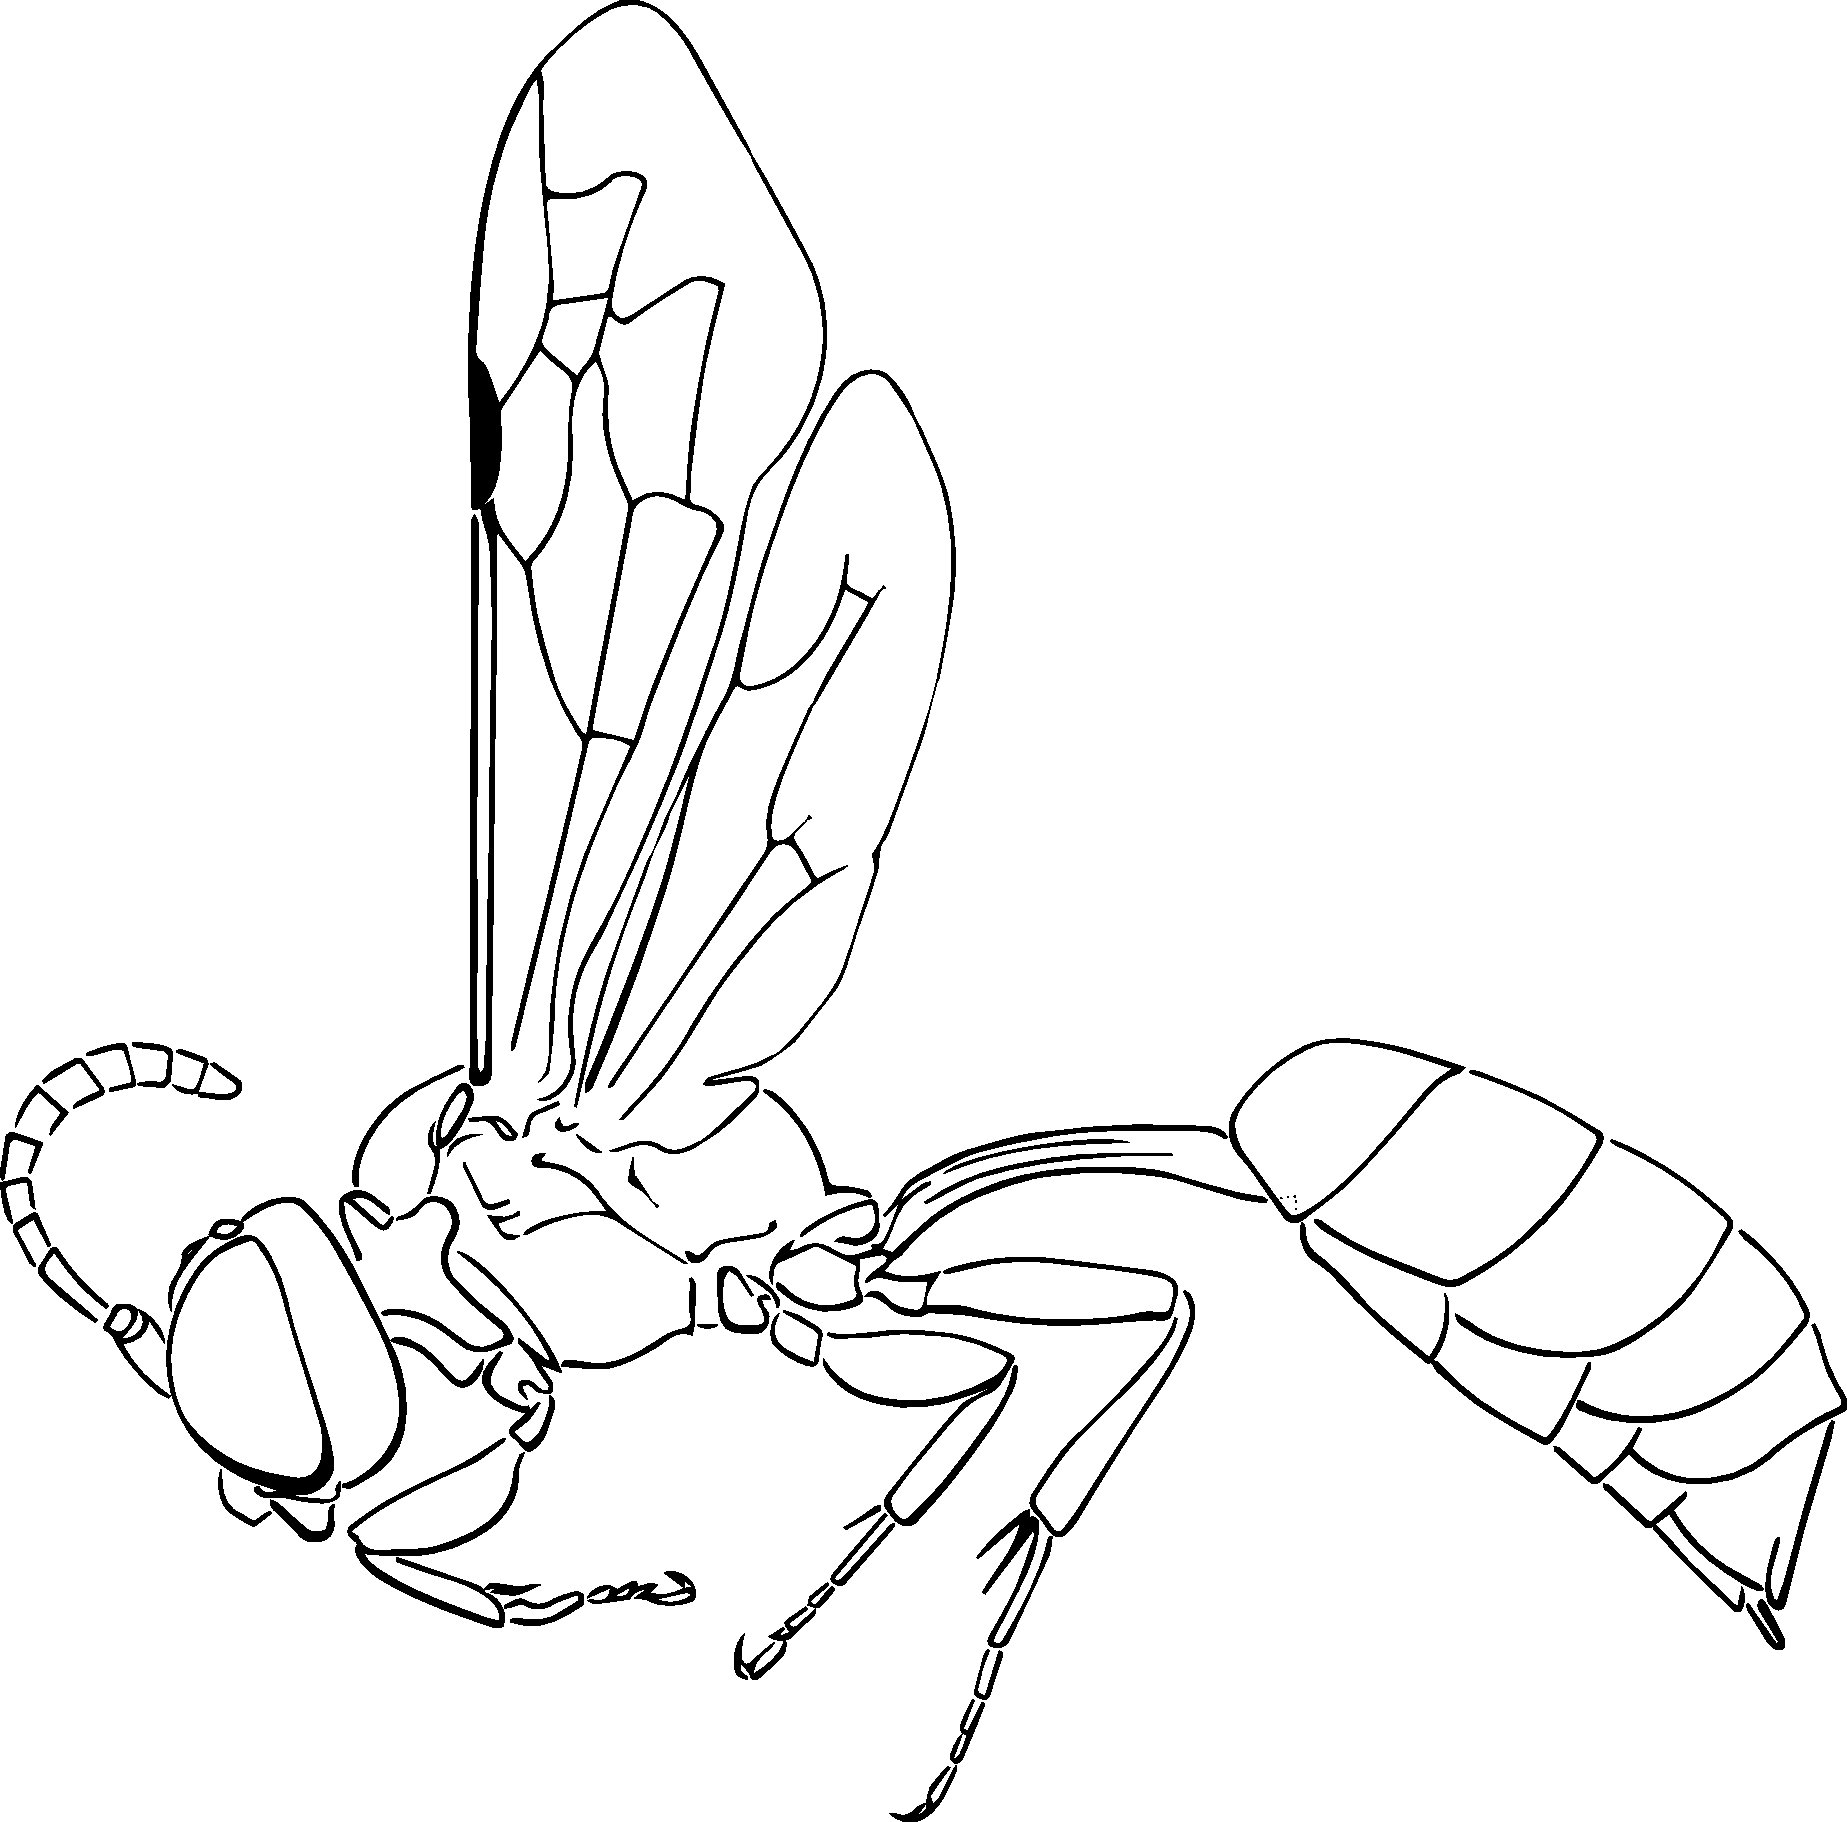
\includegraphics[width=\textwidth]{hymenoptera/CrabronidHabitus1}}
        \caption{}
        \label{fig:crabronid1}
    \end{subfigure}
    \qquad
    \begin{subfigure}[ht!]{0.38\textwidth}
        \reflectbox{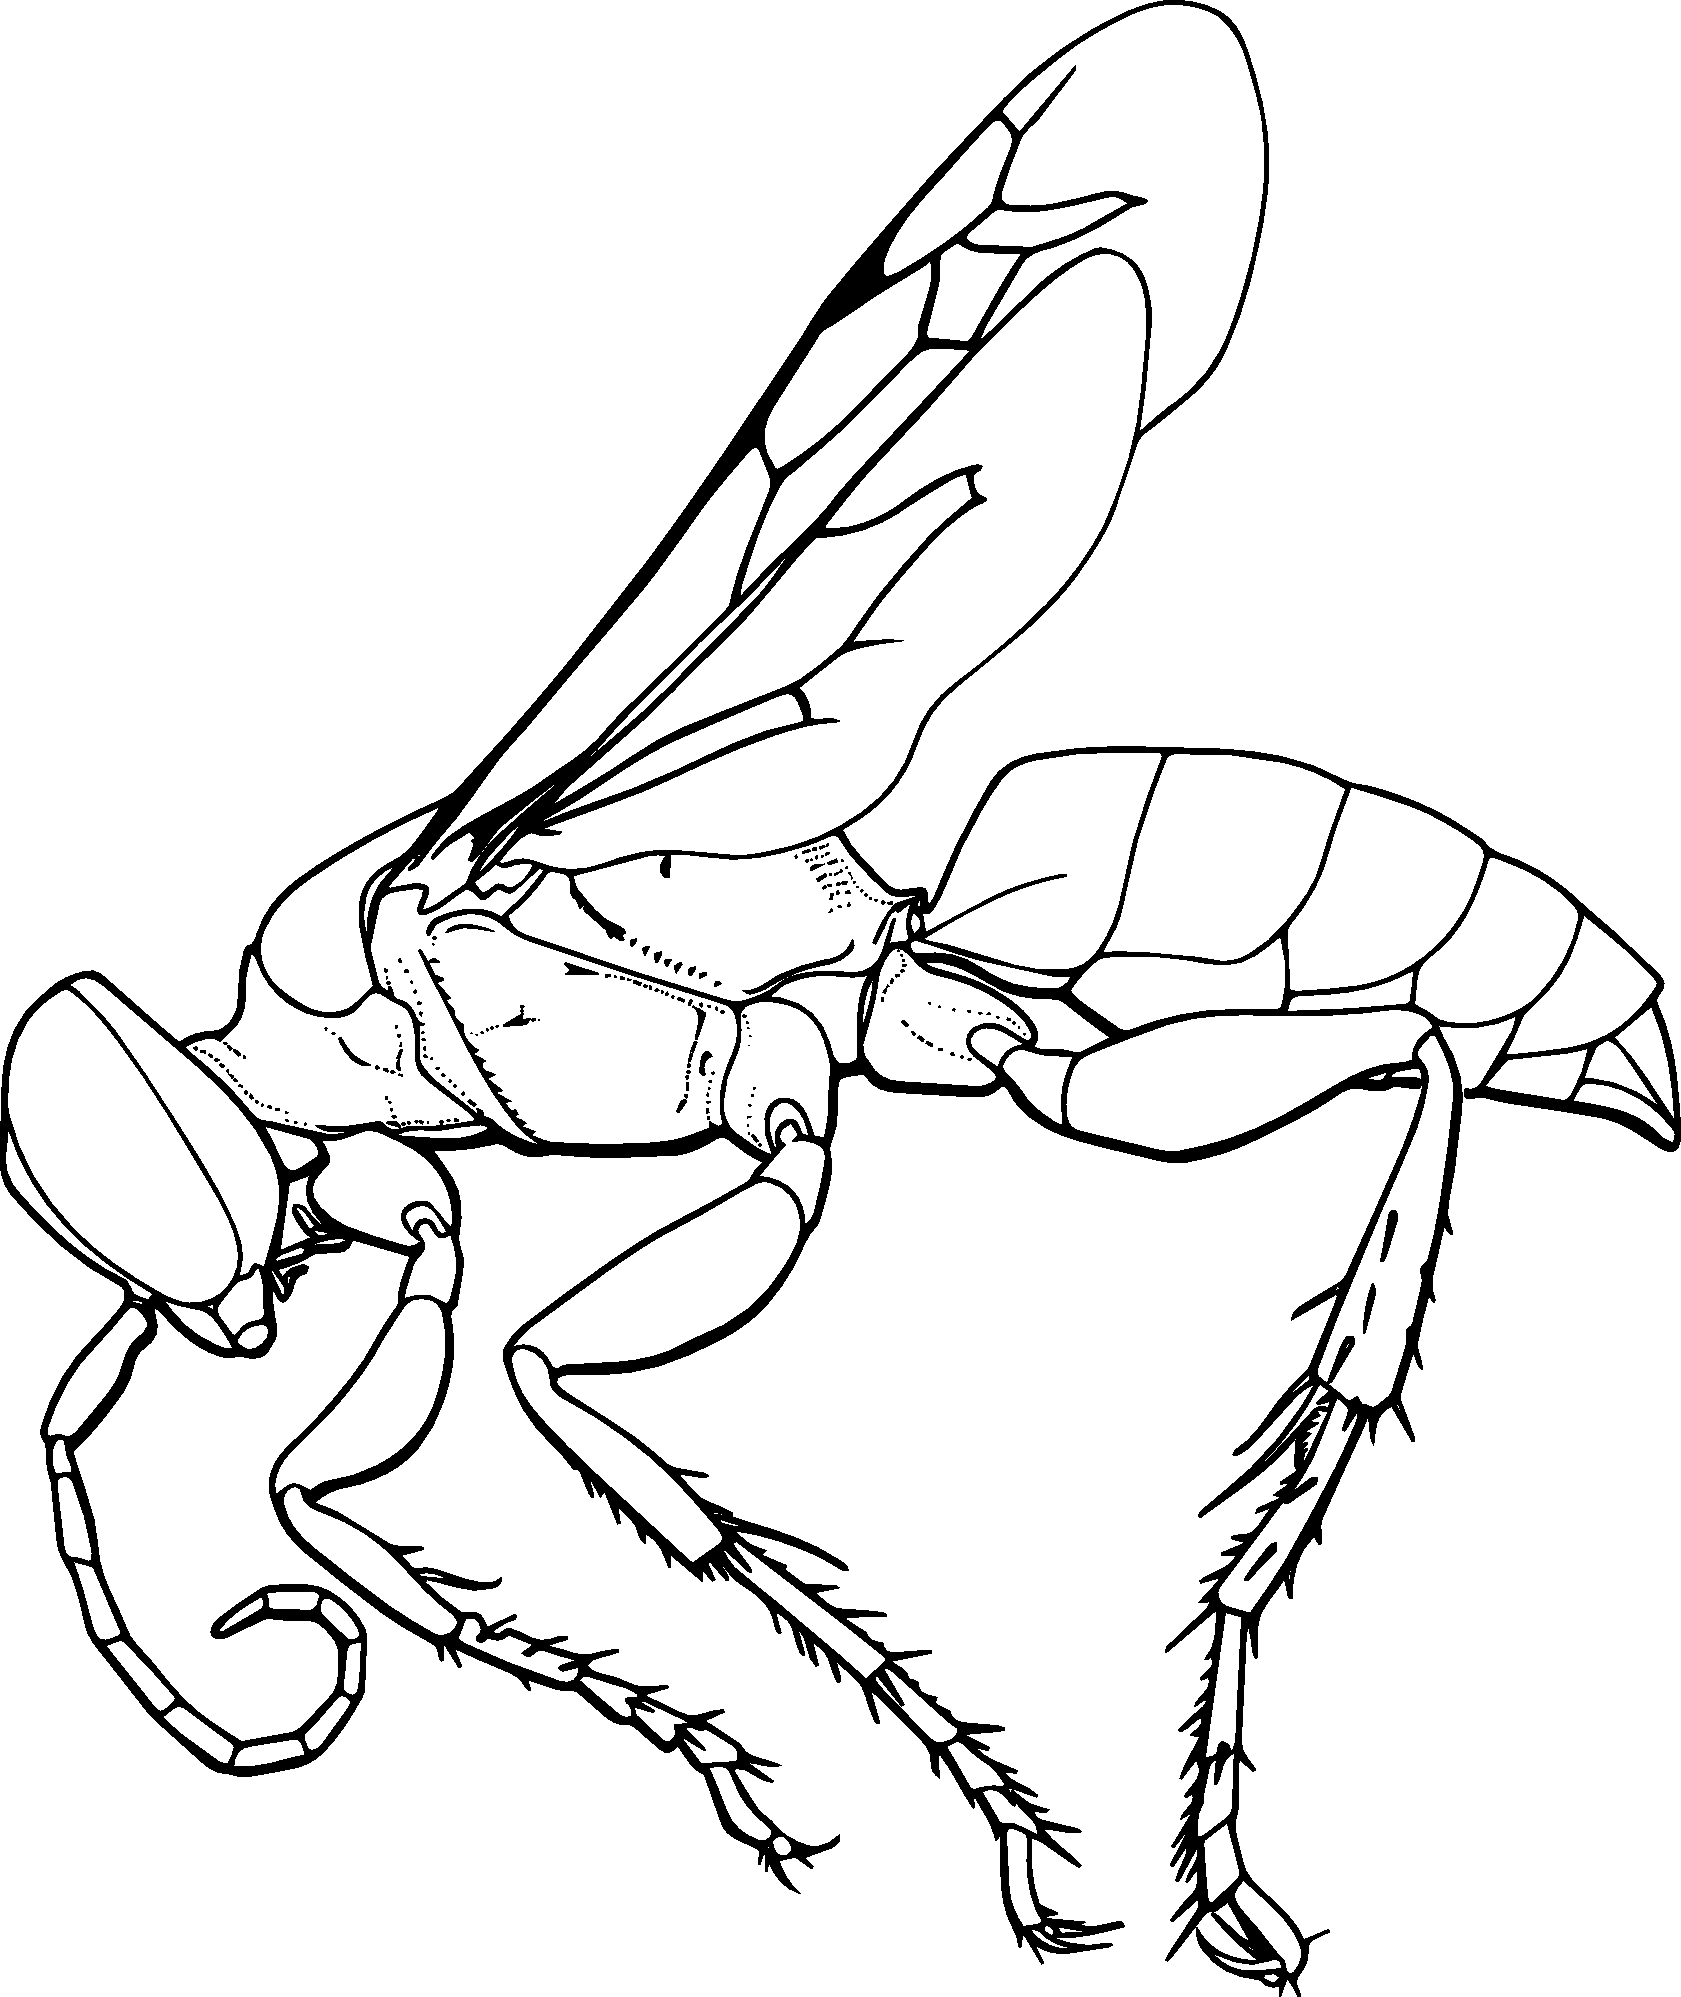
\includegraphics[width=\textwidth]{hymenoptera/CrabronidHabitus2}}
        \caption{}
        \label{fig:crabronid2}
    \end{subfigure}
    \caption{Crabronidae. \textbf{(a)} Pemphredoninae habitus \citep[][Fig. 99]{goulet1993hymenoptera}; \textbf{(b)} Larrinae habitus \citep[][Fig. 102]{goulet1993hymenoptera}}\label{fig:crabronids}
\end{figure}
\FloatBarrier

\paragraph*{Apoidea: Anthophila} The remaining families comprise the bees. All have branched setae on their bodies (lost in some cleptoparasitic species) and usually have (in females) some kind of pollen-carrying structure on the hind legs or abdomen.\index{Anthophila}\vspace{3mm}

\subsubsection{Halictidae (sweat bees)}\index{Halictidae}
\noindent{}\textit{Diagnostic characters:} Hind leg basitarsus much wider than subsequent tarsomeres; face with one subantennal suture; proboscis short; jugal lobe of hind wing long; basal vein of fore wing strongly arched (figure \ref{fig:halict1}); small to medium-sized, often metallic.\vspace{3mm}

\noindent{}\textit{Natural history:} Halictids generally nest in the soil or in rotting wood, and some species are facultatively eusocial. At least 2,000 species have been described.

\begin{figure}[ht!]
    \centering
    \begin{subfigure}[ht!]{0.26\textwidth}
        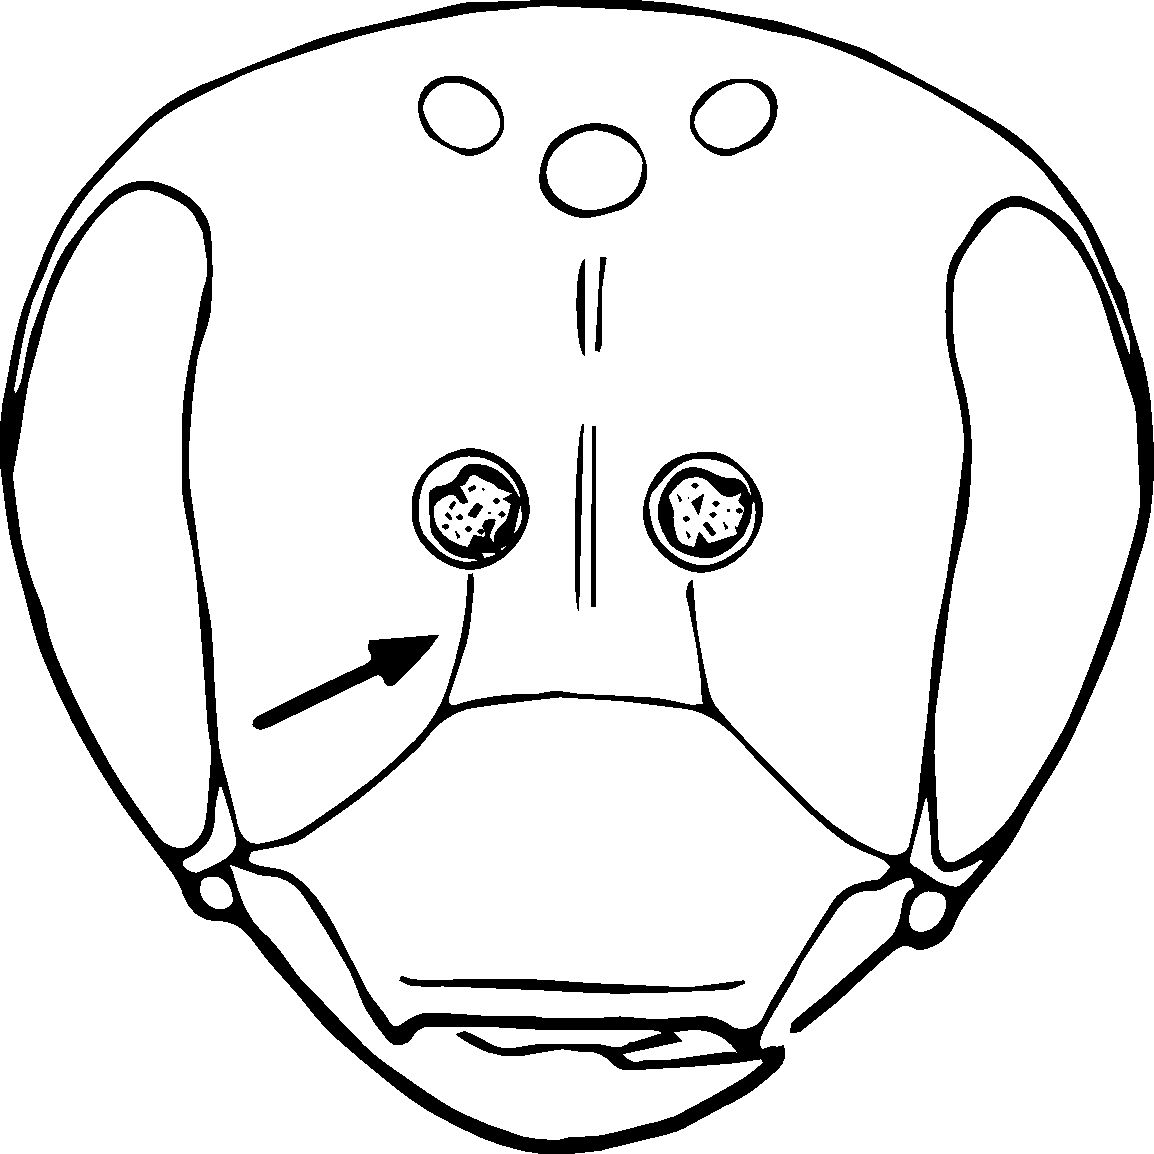
\includegraphics[width=\textwidth]{hymenoptera/HalictidFace}
        \caption{}
        \label{fig:halict1}
    \end{subfigure}
    \qquad
    \begin{subfigure}[ht!]{0.4\textwidth}
        \reflectbox{\includegraphics[width=\textwidth]{hymenoptera/HalictidHabitus}}
        \caption{}
        \label{fig:halict2}
    \end{subfigure}
    \caption{Halictidae. \textbf{(a)} Face \citep[][pg. 315]{goulet1993hymenoptera}; \textbf{(b)} habitus \citep[][Fig. 118]{goulet1993hymenoptera}}\label{fig:halictidae}
\end{figure}

\subsubsection{Andrenidae (mining bees)}\index{Andrenidae}
\noindent{}\textit{Diagnostic characters:} Proboscis short; face with two subantennal sutures (figure \ref{fig:andrenid1}, double arrow) and often with facial foveae (figure \ref{fig:andrenid1}, single arrow); jugal lobe of hind wing long; basal vein of fore wing not strongly arched; small to medium-sized, often (not always!) with hairier thorax than halictids.\vspace{3mm}

\noindent{}\textit{Natural history:} These bees typically nest in the soil. None is eusocial, as far as is known, but some species nest communally. There are $\sim$2,100 described species.

\begin{figure}[ht!]
    \centering
    \begin{subfigure}[ht!]{0.26\textwidth}
        \includegraphics[width=\textwidth]{hymenoptera/AndrenidFace}
        \caption{}
        \label{fig:andrenid1}
    \end{subfigure}
    \qquad
    \begin{subfigure}[ht!]{0.35\textwidth}
        \reflectbox{\includegraphics[width=\textwidth]{hymenoptera/AndrenidHabitus}}
        \caption{}
        \label{fig:andrenid2}
    \end{subfigure}
    \caption{Andrenidae. \textbf{(a)} Head in anterior view \citep[][pg. 313]{goulet1993hymenoptera}; \textbf{(b)} habitus \citep[][Fig. 116]{goulet1993hymenoptera}}\label{fig:andrenids}
\end{figure}

\subsubsection{Megachilidae (mason, leafcutter bees, \textit{etc}.)}\index{Megachilidae}
\noindent{}\textit{Diagnostic characters:} Proboscis rather long; jugal lobe of hind wing short; fore wing with two submarginal cells, usually equal in length; females with scopa (pollen carrier) on ventral surface of metasoma; variable in color and shape, but often ``chunkier'' than other bees.\vspace{3mm}

\noindent{}\textit{Natural history:} These bees usually nest in cavities, fro example holes in wood, and have common names that reflect the materials they use to line nests: carder (plant or animal hairs), mason (resin or soil), or leaf cutter (leaves) bees. All known species are solitary or communal. There are more than 2,000 species worldwide.

\begin{figure}[ht!]
    \centering
     \begin{subfigure}[ht!]{0.4\textwidth}
        \reflectbox{\includegraphics[width=\textwidth]{hymenoptera/MegachilidHabitus}}
        \caption{Megachilidae}
        \label{fig:megachilid1}
    \end{subfigure}
   \qquad
    \begin{subfigure}[ht!]{0.28\textwidth}
        \reflectbox{\includegraphics[width=\textwidth]{hymenoptera/ApidHabitus}}
        \caption{Apidae}
        \label{fig:apid1}
    \end{subfigure}
    \caption{Bees \citep[][Figs. 116, 123]{goulet1993hymenoptera}}\label{fig:notused}
\end{figure}

\subsubsection{Apidae (cuckoo, nomad, carpenter, bumble, honey bees, \textit{etc}.)}\index{Apidae}
\noindent{}\textit{Diagnostic characters:} Tongue long, maxillary palps vestigial; jugal lobe of hind wing usually absent; fore wing with three submarginal cells; hind tibiae usually with a scopa.\vspace{3mm}

\noindent{}\textit{Natural history:} Apidae is by far the most diverse family of bees, with \textgreater5,700 species described worldwide. These bees range from solitary (\textit{e.g.}, carpenter bees) to primitively eusocial (bumble bees) to highly eusocial (honey and stingless bees).\vspace{3mm}

\noindent{}As you have now seen, almost all bees are covered in plumose or branched setae and have special structures for carrying pollen. (Note: There are some species of cleptoparasitic bees that lack these structures.) Take a close look at the setae. Are they uniform in size and shape? How many specialized structures can you find on the body that you hypothesize might be involved in pollen collection? Based on the morphology, can you envision how pollen collection works from a behavioral perspective?\vspace{3mm}

\section*{Test yourself}
Given what you observed and what we discussed, what adaptations contributed to such a large radiation? How does this diversity look phylogenetically?\vspace{5mm}

\noindent{}How do \latinword{idiobiont} parasitoids differ from \latinword{koinobiont} parasitoids?\vspace{5mm}

\noindent{}Can you describe how these arthropods live (natural history) and roughly how diverse they are---Apocrita, Aculeata, Orussidae? Do you know how they're related to one another? 


\clearpage
\thispagestyle{empty}